\documentclass[12pt, twoside, final, openany]{mgr}
\usepackage[T1]{fontenc}
\usepackage[polish]{babel}
\usepackage[UTF8]{inputenc}
\usepackage{lmodern}
%\usepackage{indentfirst}
\usepackage{pbox}
\usepackage{courier}

%pakiety do grafiki
\usepackage{graphicx}
\usepackage{subcaption}
\usepackage{psfrag}
\usepackage{textcomp}
%do pierwszej strony
\usepackage{pdfpages}

%pakiety dodające dużo dodatkowych poleceń matematycznych
\usepackage{amsmath}
\usepackage{amsfonts}

%pakiety wspomagające i poprawiające składanie tabel
\usepackage{supertabular}
\usepackage{array}
\usepackage{tabularx}
\usepackage{hhline}
\usepackage{float}
%pakiet wypisujący na marginesie etykiety równań i rysunków
%\usepackage{showlabels}

%definicje własnych poleceń
\newcommand{\R}{I\!\!R} %symbol liczb rzeczywistych, działa tylko w trybie matematycznym
\renewcommand*\descriptionlabel[1]{\hspace\leftmargin$#1$}
\newtheorem{theorem}{Twierdzenie}[section] %nowe otoczenie do
                                           %składania twierdzeń
\newcommand{\chartsWidth}{0.80}
%dane do złożenia strony tytułowej
%\title{Analiza łańcucha transakcji w sieci Bitcoin}
%\engtitle{The analysis of Bitcoin transactions blockchain}
%\author{Bartosz Zychal}
%\supervisor{dr inż. Radosław Michalski} %\Prof. PWr, I-6
%\guardian{dr hab. inż. Imię Nazwisko Prof. PWr, I-6} %nie używać
%jeśli opiekun jest tą samą osobą co prowadzący pracę
%\date{2018} %standardowo u dołu strony tytułowej umieszczany jest
%bieżący rok, to polecenie pozwala wstawić dowolny rok
%poniżej jest lista kierunków i specjalności na wydziale elektroniki,
%należy wybrać właściwe lub dopisać jeśli nie ma odpowiednich
%\field{Informatyka (INF)}
%\specialisation{Systemy Baz Danych (SBD)}

%tutaj zaczyna się właściwa treść dokumentu
\begin{document}
\def\listtablename{Spis tabel. }
\def\tablename{Tabela. }
%\maketitle %polecenie generujące stronę tytułową 
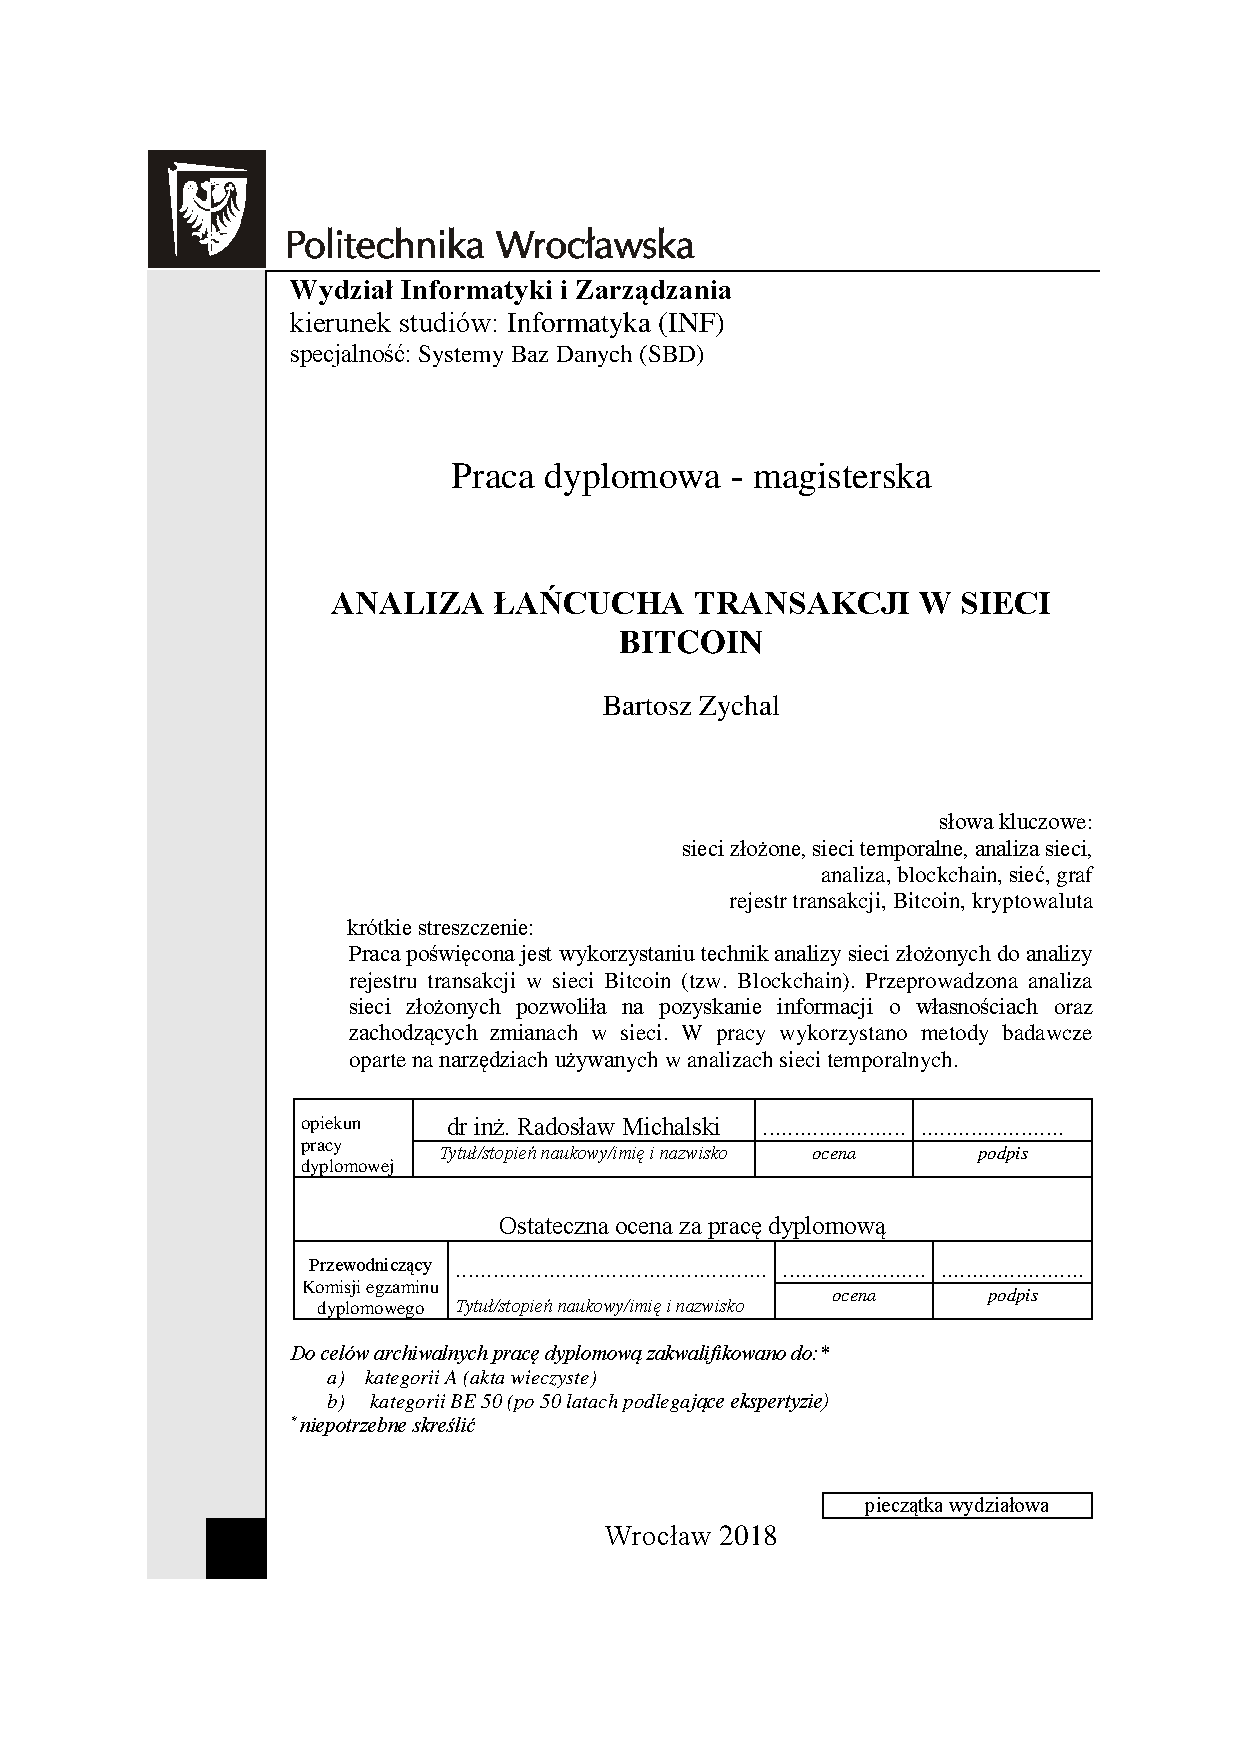
\includepdf[scale=1,pages=1]{pictures/title.pdf}


\tableofcontents{2} 
%spis treści
\chapter*{Wprowadzenie}
\addcontentsline{toc}{chapter}{Wprowadzenie}
\vspace{-1ex}
\indent Celem pracy jest wykorzystanie technik analizy sieci złożonych do analizy rejestru transakcji w sieci Bitcoin (tzw. Blockchain). W pracy podjęta została próba odpowiedzi na pytanie, jakie własności transakcji można pozyskać wykorzystując analizę sieci złożonych.

\indent Problem badawczym pracy jest próbkowanie oraz eksploracja sieci złożonych. Istotnym zagadnieniem jest również tempo rozwoju sieci użytej do przeprowadzenia badań, które cały czas rośnie. Wymusza to, obok badania właściwości, badanie trendów zmian w sieci.

\indent Obiektem badań wykorzystanym na potrzeby realizacji pracy jest sieć zbudowana na podstawie mechanizmu zawartego w jednej z kryptowalut. Cała sieć jest rzeczywistą siecią złożoną, składającą się z prawie trzystu tysięcy połączeń oraz milionów węzłów, dlatego też jej rozmiar obliguje do zastosowania określonych metod badawczych.

\indent Praca opiera się na metodach badawczych stosowanych w badaniu temporalnych sieci złożonych. Metody te charakteryzują się rozszerzeniem klasycznego konceptu sieci złożonej o dodatkowy wymiar, jakim jest czas. Na potrzeby przeprowadzenia badań wybrano sto momentów istnienia sieci Bitcoin, a następnie wykonano szereg analiz.

\indent Rosnąca popularność kryptowalut, a zarazem duża liczba kontrowersji, które pojawiły się w ostatnich latach sprawiają, że tematem Bitcoina zainteresowało się wiele kręgów naukowych z różnych dziedzin. Naukowcy podejmują tematy od analizy bezpieczeństwa struktury, przez anonimowość do wyodrębnienia stałych oraz ewoluujących właściwości sieci. Największe zainteresowanie wzbudza anonimowość w sieci Bitcoin. W wielu pracach podejmuje się próbę korelacji zachowań użytkowników z przeprowadzanymi transakcjami przy jednoczesnym dopasowaniu do informacji spoza systemu. Wyniki tych badań wskazują, że źródło sukcesu kryptowaluty - anonimowość - jest tylko pozorne. Poza kwestią bezpieczeństwa naukowcy poruszają tematy związane z przemianami następującymi w~sieci. Istnieje wiele publikacji, w~ramach których bada się wyłącznie początek istnienia sieci, co w związku z narastającą ciekawością społeczeństwa może być niewystarczające. W niniejszej pracy podjęto się czasowej analizy sieci Bitcoin, która przedstawia właściwości oraz przemiany w sieci, w latach \textit{2015-2017}.

\indent W rozdziale \ref{kryptowaulty} przedstawiono ideę oraz mechanizm działania kryptografii. Ponadto zaprezentowano sposób wykorzystania kryptografii w kryptowalutach oraz opisano model bezpieczeństwa zapewniany przez kryptowaluty na przykładzie sieci Bitcoin.

\indent Rozdział \ref{blockchain} odwołuje się do sposobu realizacji transakcji w sieci Bitcoin poprzez wpisanie jej do globalnego rejestru transakcji. Zawiera informacje odnośnie struktury Blockchain'a, pojedynczego bloku oraz transakcji. Dodatkowo przedstawiony został proces dołączania kolejnego bloku z transakcjami do Blockchain'a.

\indent Metody analizy sieci zaprezentowane zostały w rozdziale \ref{przegladAnalizy} wraz z przeglądem powiązanych prac badawczych dotyczących Blockchain'a. W rozdziale tym zawarto również zakres przeprowadzanych badań w ramach pracy.

\indent W rozdziale \ref{analizaBlockchain} opisano przeprowadzone badania oraz zaprezentowano otrzymane wyniki, na podstawie których wyciągnięto wnioski.

\chapter{Kryptowaluty - wprowadzenie}
\label{kryptowaulty}
\section{Wprowadzenie} 
\label{sec:KryptowalutyWprowadzenie}
\indent Rolą niniejszego rozdziału jest wyjaśnienie istoty oraz sposobu działania kryptowalut. Przedstawiono w nim, czym są kryptowaluty oraz kryptografia, w jaki sposób kryptowaluty korespondują z kryptografią oraz w jaki sposób kryptografia pozwala zapewnić wysokie bezpieczeństwo kryptowaluty. Na przykładzie jednej z najpopularniejszych walut cyfrowych, tj. Bitcoina, zaprezentowano zastosowanie kryptografii na potrzeby jej zabezpieczenia.

\section{Definicja} \label{sec:definicjaKryptowaluty}
\indent Krypotowaluta to cyfrowy zasób mogący odpowiadać pewnej wartości środków finansowych. Zasób ten został zaprojektowany w sposób pozwalający określać go jako medium wymiany przy użyciu kryptografii, z którą jest ściśle powiązany. Kryptografia pozwala na zabezpieczenie transakcji, kontrolowanie tworzenia nowych jednostek kryptowaluty oraz weryfikację ilości posiadanych jednostek. Aktualnie krypotwaluty klasyfikowane są do trzech grup:
\begin{itemize}
\item[--] walut cyfrowych,
\item[--] walut alternatywnych,
\item[--] walut wirtualnych.
\end{itemize}

\section{Bezpieczeństwo w walutach i kryptowalutach} \label{sec:bezpieczenstwoWwalutach}
\indent Wszystkie waluty muszą być w jakiś sposób kontrolowane i podlegać różnego rodzaju zabezpieczeniom, tak aby zapobiegać oszustwom. W przypadku walut fiducjarnych, tj. walut nie mających pokrycia w dobrach materialnych, organizacje takie jak banki kontrolują podaż pieniądza oraz oznaczają fizycznie walutę, w celu uniemożliwienia jej podrobienia. Takie zabezpieczenia w pewnym stopniu ograniczają możliwości fałszerstwa, jednakże nie dają stuprocentowej pewności. Kryptowaluty podobnie jak tradycyjne waluty muszą posiadać miary zabezpieczeń w celu uniemożliwienia wpływania na stan systemu i tworzenia niekonsystentnych danych. Dodatkowo muszą one posiadać zabezpieczenia niepozwalające na wielokrotne użycie tych samych środków. W przeciwieństwie do walut fiducjarnych zasady bezpieczeństwa kryptowalut mogą bazować wyłącznie na istniejących technologiach i nie muszą podlegać kontroli ze strony jakiejkolwiek centralnej instytucji\cite{elektrInstruBezEmitenta}.

\section{Kryptografia} \label{sec:kryptografia}
\indent Kryptowaluty bardzo silnie bazują na kryptografii, która oferuje mechanizm bezpiecznego kodowania zasad ich systemu. Kryptografia pozwala nie tylko bronić system przed manipulacjami i matactwami, ale równie dobrze może zostać użyta w celu kodowania zasad tworzenia nowych jednostek kryptowaluty przy pomocy określonego matematycznego protokołu\cite{Cryptocurrency}. 

\indent Kryptografię można sklasyfikować jako dziedzinę wiedzy o zabezpieczeniach przed nieautoryzowanym dostępem do informacji. W dzisiejszych czasach uważa się ją nie tylko za gałąź matematyki, ale i informatyki. Kryptografię można podzielić na:
\begin{itemize}
\item[A.] Symetryczną - polega na możliwości odczytania wiadomości przy pomocy tego samego klucza, którym została podpisana. Znaczącym problemem bezpieczeństwa w~tym podejściu jest przekazanie odbiorcy klucza. 
\item[B.] Niesymetryczną\cite{CryptoDenga, asynchModel} - polega na istnieniu co najmniej dwóch kluczy:
\begin{itemize}
\item[--] Prywatny - klucz ten nie powinien być nigdy nikomu udostępniony. Przy pomocy klucza prywatnego można odszyfrować wiadomość podpisaną kluczem publicznym. Pozwala również na podpisanie wiadomości, która może być później zweryfikowana za pomocą klucza publicznego.
\item[--] Publiczny - klucz ten może zostać bez żadnych zastrzeżeń upubliczniony. Klucz publiczny tworzy się na podstawie klucza prywatnego, jednakże odtworzenie klucza prywatnego z klucza publicznego jest bardzo trudne. Klucz publiczny używany jest do szyfrowania wiadomości oraz weryfikacji wiadomości podpisanej kluczem prywatnym.
\end{itemize}
\end{itemize} 

\indent Kryptografia oparta na kluczu publicznym została opracowana w latach 70. XX wieku i cały czas stanowi solidną podstawę bezpieczeństwa komputerowego i informacyjnego. Od czasu jej powstania odkryto funkcje matematyczne, które są praktycznie nieodwracalne, (np. \textit{potęgowanie liczby pierwszej} i \textit{mnożenie krzywych eliptycznych}), co oznacza, że łatwo obliczyć je w jednym kierunku, jednakże operacja odwrotna jest praktycznie niewykonywalna. Bitcoin korzysta z mnożenia krzywej eliptycznej jako podstawy przy wyliczaniu klucza publicznego. W podrozdziale~\ref{sec:tworzenieKluczyPublicznych} przedstawiono sposób użycia tej funkcji.

\section{Zastosowanie kryptografii w sieci Bitcoin} \label{sec:zastosowanieKryptografii}
\indent Aktualnie na rynku dostępne jest ponad tysiąc różnych kryptowalut, a wraz z rosnącym zainteresowaniem oraz zaufaniem społecznym ilość walut cyfrowych cały czas rośnie\cite{Zcoinmarketcap, TheAgeOfCryptocurrency}. Niepodważalny jest fakt, że jedną z najbardziej powszechnych i popularnych kryptowalut jest Bitcoin. Bitcoin jest całkowicie zdecentralizowaną, zdigitalizowaną walutą bez globalnego emitenta, który miałby nią zarządzać oraz ją rozpowszechniać. Bazując na specjalistycznym otwartym oprogramowaniu pewna ilość bitcoinów przekazywana jest użytkownikom w zamian za działania pozwalające na poprawne funkcjonowanie systemu Bitcoin. Użytkownicy ci zwani są kopaczami lub górnikami, a operacje przez nich wykonywane, w celu podtrzymania systemu, zwane są kopaniem. Kopanie bitcoinów, poza zyskiem ze strony kopaczy, daje olbrzymi zysk dla systemu, pozwalając weryfikować zlecone transakcje.

\indent Właściciele bitcoinów ustalani są na podstawie kluczy cyfrowych, adresów Bitcoin oraz podpisów cyfrowych. Klucze cyfrowe nie są przechowywane w sieci, jednakże są tworzone przez użytkowników oraz przetrzymywane w ich portfelach, w plikach lub bazie danych. Klucz cyfrowy jest całkowicie niezależny od protokołu sieci Bitcoin, dlatego też może być tworzony przez różnie oprogramowania. Oprogramowanie to musi zapewniać użycie bezpiecznego źródła entropii w celu wygenerowania unikalnego klucza\cite{Mastering, asychPrivateKey}. Wygenerowanie istniejącego lub zbyt słabego klucza może spowodować, iż w przyszłości użytkownik utraci zebrane środki. Klucze zapewniają w sieci Bitcoin:
\begin{itemize}
\item[--] zdecentralizowane zaufanie,
\item[--] zaświadczenie o własności,
\item[--] odporny na kryptografię model bezpieczeństwa.
\end{itemize}
Transakcje w sieci Bitcoin wymagają dodania prawidłowego podpisu do łańcucha bloków, co dokładniej zostało opisane w rozdziale~\ref{blockchain}. Podpis ten może być wygenerowany przy pomocy ważnych kluczy cyfrowych. Każdy kto posiada kopię tych kluczy może kontrolować środki dostępne na koncie. Protokół sieci Bitcoin korzysta z szyfrowania asymetrycznego, co w konsekwencji oznacza, że w transakcji klucz publiczny odbiorcy jest prezentowy przez jego odcisk palca, zwany adresem Bitcoin. Adresy te są ogólnodostępne i widoczne przez wszystkich\cite{blockchaininfo}. 

\indent Z klucza publicznego korzysta się w celu odebrania Bitcoinów, natomiast klucz prywatny wymagany jest do wydawania Bitcoinów. Osoba wydająca Bitcoiny musi zaprezentować swój klucz publiczny oraz podpis w transakcji. Podpis za każdym razem jest inny, lecz tworzony z jednego klucza prywatnego, co pozwala na udaną weryfikację przy pomocy dołączonego klucza publicznego. Poprzez załączenie obu tych informacji każdy w sieci może zweryfikować oraz zaakceptować transakcję jako poprawną lub ją odrzucić w przypadku stwierdzenia, braku środków na adresie nadawcy. 

\indent Klucz prywatny w sieci Bitcoin powiązany jest ścisłe z adresem, dlatego też jego utrata powoduje nieodwracalną utratę środków. Pomimo iż środki są cały czas dostępne, nie mogą zostać użyte bez prawidłowego podpisu generowanego z klucza prywatnego.

\section{Metoda tworzenia kluczy publicznych na przykładzie sieci Bitcoin} \label{sec:tworzenieKluczyPublicznych}
\indent Jak już wcześniej wspomniano klucz publiczny obliczany jest z klucza prywatnego przy pomocy \textit{mnożenia krzywej eliptycznej}. Metoda ta została szczegółowo opisana przez \textit{Andreas M. Antonopoulos}\cite{Mastering}, jednakże w celu przedstawienia siły zabezpieczenia, jakie daje szyfrowanie asymteryczne, przedstawiono ją poniżej w skróconej formie. 

\indent Klucz publiczny jest praktycznie nieodwracalny i sposób jego wyliczania można zapisać jako:
\begin{equation}
\label{eq:1}
  K = k*G, 
\end{equation} 
gdzie:
\begin{description}
\item[k] jest wartością klucza prywatnego,
\item[G] jest stałym punktem zwanym punktem generującym,
\item[K] jest wynikowym kluczem publicznym.
\end{description}

Kryptografia krzywej eliptycznej jest rodzajem kryptografi asymetrycznej bazującej na problemie logarytmu dyskretnego wyrażonego jako sumy i iloczyny punktów na tej krzywej eliptycznej. Dlatego też, operacją odwrotną do mnożenia krzywej eliptycznej jest \textit{odnalezienie logarytmu dyskretnego}, co wymaga zastosowania wyszukiwania przy pomocy algorytmu typu \textit{brute-force}, czyli przeglądu zupełnego.

\indent W przypadku Bitcoina parametry krzywej eliptycznej są ściśle określone i zdefiniowane przy pomocy standardu zwanego \textit{secp256k1}. Standard ten został ustalony przez amerykańską Narodową Instytucję Standaryzacji i Technologii. Zastosowana w tej kryptowalucie krzywa eliptyczna tworzona jest na podstawie określonego zbioru stałych matematycznych i jest wyrażana przy pomocy funkcji:
\begin{equation}
  y^2 = x^3 + 7 
\end{equation} 
\label{eq:2}
lub:
\begin{equation} 
\label{eq:3}
  y2 \mod p = (x^3 + 7) \mod p
\end{equation}
Moduł liczby pierwszej \textit{mod p} implikuje właściwość krzywej jako znajdującej się nad skończonym polem pierwszego rzędu p. Można ją również zapisać jako funkcję $F_p$, gdzie $p = 2^{256} - 2^{32} - 2^9 - 2^8 - 2^7 - 2^6 - 2^4 - 1$ jest olbrzymią liczbą pierwszą. Oznacza to, że od pewnego momentu krzywa zdefiniowana jest przy pomocy liczb zespolonych, a nie rzeczywistych. Utrudnia to jej wizualizację, gdyż wykres takiej funkcji musiałby zostać przedstawiony w dwóch wymiarach i~składałby się z~wielu pojedynczych punktów w~przestrzeni. Na potrzeby graficznego przedstawienia uproszczono wykres~\ref{fig:krzywaEliptyczna} funkcji~\ref{eq:2} przedstawiając go tylko w świecie liczb rzeczywistych. Wykres ten został podzielony na dwa obszary przy pomocy pionowej kreski, która nie jest częścią wykresu funkcji. Lewy obszar obejmuje wartości funkcji w świecie liczb zespolonych, który pominięto, natomiast prawa strona wykresu przedstawia funkcję~\ref{eq:2} w świecie liczb rzeczywistych.

\indent Parametr \textit{G} został wybrany na podstawie krzywej eliptycznej - przedstawionej na wykresie~\ref{fig:krzywaEliptyczna} - przez protokół Bitcoina przy użyciu standardu \textit{secp256k1}. Parametr ten jest przypisywany do wszystkich użytkowników sieci. Determinuje to wygenerowanie za każdym razem takiego samego klucza publicznego na podstawie tego samego klucza prywatnego. Klucz prywatny może mieć wartość od $1$ do prawie $2^{256}$, a zależność pomiędzy jego wartością \textit{k} i wartością klucza publicznego \textit{K} jest stała. Oznacza to, że aby przy znajomości stałej wartości \textit{G} odtworzyć wartość klucza publicznego \textit{K} wymagany jest przegląd wszystkich możliwych wartości klucza prywatnego \textit{k}. 

\newpage
\vfill
\begin{figure}[!h]
\centering
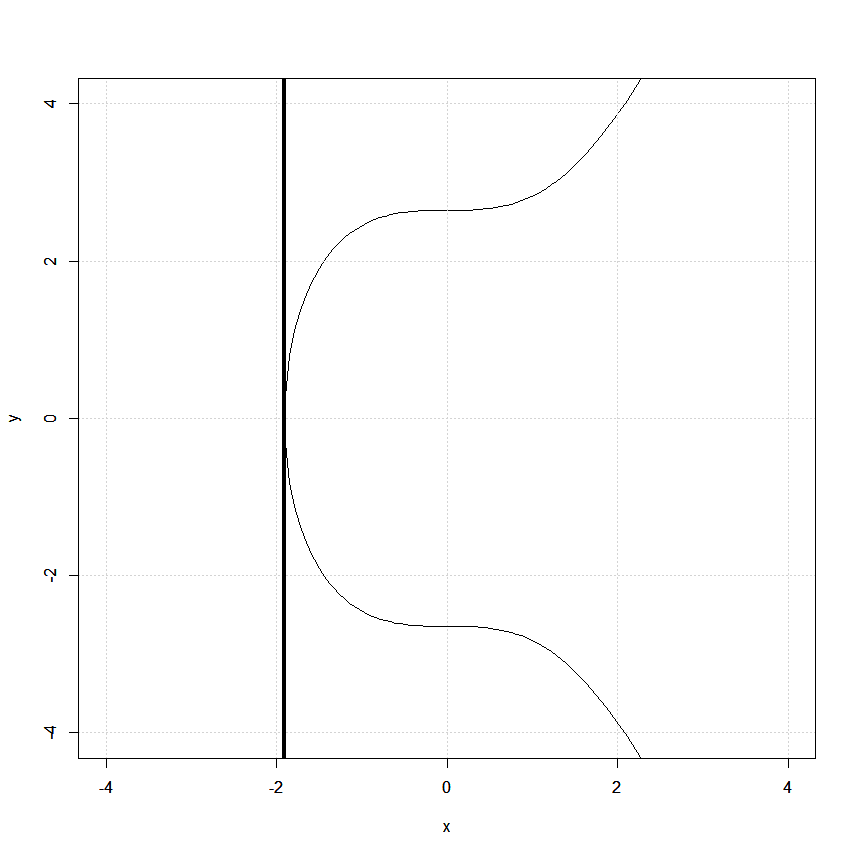
\includegraphics[width=0.9\linewidth]{pictures/elliptic.png}
\caption{Krzywa eliptyczna zastosowana do wyznaczenia wartości G w protokole Bitcoin}
\label{fig:krzywaEliptyczna}
\end{figure}

\section{Podsumowanie} \label{sec:podsumowanieKryptowaluty}
\indent Reasumując, za każdą walutą musi stać określony system zabezpieczeń. W przypadku tradycyjnych walut są to centralne instytucje nadzorujące obrót i podaż określonego pieniądza. W przypadku kryptowalut bezpieczeństwo zapewnione jest poprzez zastosowanie prostej w użyciu, aczkolwiek skomplikowanej w budowie kryptografii. Zapewnia to możliwości bardzo szybkiej weryfikacji posiadanych środków przy bardzo niskim nakładzie pracy. Dodatkowo kryptografia, w porównaniu do tradycyjnych metod zabezpieczania pieniądza, nie pozwala na kontrolowanie przez jedną osobę, organizację czy instytucję poprawności danych. To zadanie wykonywane jest przez wszystkich kopaczy w sieci Bitcoin. 


\chapter{Blockchain - rejestr transakcji}
\label{blockchain}

\section{Wprowadzenie}
\indent W tym rozdziale przedstawiono oraz wyjaśniono ideę rejestru transakcji, tzw. Blockchain'a. Opisano strukturę bloku, transakcji oraz wejść i wyjść w transakcji. Rozdział ten opisuje również w jaki sposób tworzone są transakcje, jak są weryfikowane i jakie koszty ponosi się za przekazanie Bitcoinów innemu uczestnikowi sieci. Dodatkowo przedstawiono proces tworzenia oraz dodawania nowego bloku do Blockchain'a. 

\section{Definicja Blockchain'a}
\label{definicjaBlockchaina}
\indent Łancuch bloków (ang. Blockchain) jest uporządkowaną strukturą, zwaną jednokierunkową listą składającą się z bloków transakcji. Listę tę charakteryzuje połączenie wsteczne, co oznacza, że blok następny wskazuje na blok poprzedni. Każdy kolejny blok ma przypisaną swoją wysokość w łańcuchu bloków. Wysokość ta ustalana jest na podstawie odległości bloku od pierwszego bloku w łańcuchu. Blok ten, zwany blokiem genezy, stanowi pierwszego \textit{rodzica} oraz wspólnego przodka dla wszystkich bloków w całym łańcuchu\cite{BitcoinAndCryptocurrencyTechnologies, BlockchainExplained, BitcoinAndTheBlockchain}. Na ilustracji~\ref{fig:lancuchBlokow} przedstawiona została idea łańcucha bloków.

\indent Pierwszy blok łańcucha bloków w sieci Bitcoin został wygenerowany w 2009 roku i~jako jedyny z bloków zapisany jest w kodzie źródłowym oprogramowania - zapewnia to zaufanego wspólnego przodka dla wszystkich bloków łańcucha.

\indent Bloki rozpoznaje się na podstawie unikalnego hash'a, który generowany jest przy użyciu algorytmu kryptograficznego SHA256\cite{sha2}. Wynikowy hash ma 256 bitów i jest prezentowany zazwyczaj w systemie heksadecymalnym, co ułatwia jego odczyt. Bloki nie zawierają swojego hash'a w~nagłówku, co komplikuje szybkie odnajdowanie konkretnego bloku. W~celu łatwej i szybkiej identyfikacji, dane o bloku muszą być przetrzymywane w bazie danych zawierającej dodatkowe informacje o łańcuchu bloków. Każdy z~węzłów sieci oblicza hash bloku w~trakcie jego odbierania. W~nagłówku blok zawiera informację tylko o~rodzicu, tzn. przechowuje hash rodzica. Poruszając się wstecz przy pomocy tych hash'y powróci się do pierwszego bloku - bloku genezy. 

\indent Hash bloku powstaje na podstawie jego zawartości włączając w to nagłówek bloku, w~którym znajduje się wspomniany hash poprzednika. Powoduje to, iż ingerencja w dane znajdujące się w blokach staje się niemożliwa ze względu na ilość obliczeń jakie należałoby wykonać, aby je zmienić. Jakakolwiek zmiana w bloku rodzica wymusza zmianę w bloku dziecka, dlatego im blok jest starszy tym jest bezpieczniejszy. Taka struktura stanowi podstawę bezpieczeństwa w sieci Bitcoin.

\indent Im blok znajduje się dalej w łańcuchu tym jest stabilniejszy i pewniejszy, natomiast ostatnie bloki, tzn. najświeższe, mogą ulegać zmianom w wyścigu prowadzonym przez kopaczy. W tym samym momencie na ostatni blok może wskazywać wiele nowych bloków wyprodukowanych w trakcie kopania. Taka sytuacja prowadzi do rozgałęzienia się łańcucha bloków. Jest to nieakceptowalne~w opisywanej strukturze, dlatego ostatecznie do łańcucha bloków dołączany zostaje jeden~z wygenerowanych bloków, a reszta bloków zostaje odrzucona. Bardziej szczegółowo problem ten został opisany w podrozdziale~\ref{dolaczanieNowegoBloku}.

\indent Szczegóły działania systemu kryptowalutowego zostały opisane w dokumencie opracowanym przez Satoshi Nakamoto\cite{nakamoto2008bitcoin}. Należy zauważyć, że nazwa Satoshi Nakoamoto powszwechnie uważana jest za pseudonim\cite{satoshi}. Satoshi Nakamoto przedstawia jako pierwszy pełną koncepcje zdecentralizowanego  systemu opartego na łańcuchu transakcji, to jest Blockchain'ie. Dodatkowe informacje dostępne są również na stronie Bitcoina oraz stronie poświęconej Bitcoinowemu Blockchain'owi\cite{blockchaininfo, bitcoinorg}.

\newpage
\begin{figure}[H]
	\begin{center}
  	\begin{tabular}{ | l  c | }
		\hline    
     	Hash bloku & \texttt{000000000000000000a7b47a1e58e456} \\
    			    & \texttt{fd54ae5a30cb92a35ca3e5acee065287} \\ 
    	Wysokość bloku & \texttt{496201} \\ 
    	Rozmiar: & \texttt{1071.607 kB} \\
   	 	Liczba transakcji: & \texttt{2032} \\ \hline
		\textbf{Nagłówek bloku}  &  \\  	 	
   	 	Wersja: & \texttt{0x20000000} \\   	 	
   	 	Hash poprzedniego bloku: &  \texttt{000000000000000000c6dd215947b569} \\
    							 &  \texttt{fa06de2cb856dec643daf5a7e8efc72e} \\ 
		Markle root: 			 & \texttt{b96da6d09865e36e4862b5a612fb1893} \\
								 & \texttt{275d889989feb5a7a217503fd84019e3} \\
   		Czas wykopania: & \texttt{2017-11-26 13:51:02} \\
   		Trudność: & \texttt{1,347,001,430,558.57}\\
   		\hline
   		Transakcje &\\
   		\hline 
 	\end{tabular}
	\end{center}
	
	\begin{center}
	\begin{tabular}{c} 
		\big\Downarrow\
	\end{tabular}
	\end{center}
	
	\begin{center}	
	\begin{tabular}{ | l  c | }
		\hline    
     	Hash bloku & \texttt{000000000000000000c6dd215947b569} \\
    			    & \texttt{fa06de2cb856dec643daf5a7e8efc72e} \\ 
    	Wysokość bloku & \texttt{496200} \\
    	Rozmiar: & \texttt{1062.264 kB} \\
		Liczba transakcji: & \texttt{1036}\\ \hline
		\textbf{Nagłówek bloku} & \\
   	 	Wersja: & \texttt{0x20000000} \\   	 
   	 	Hash poprzedniego bloku: & \texttt{000000000000000000c645c295fbd91d}\\
   	 							 & \texttt{f2f53e0346a4ecf8821abc8cc18fa4b1}\\
		Markle root: 			 & \texttt{c6be2f384d7fa195dfac1ce367ee3a9f}\\
								 & \texttt{9ccfaf9cd337b261be1a0ff0e5d73bc4}\\
   		Czas wykopania: & \texttt{2017-11-26 13:43:52}\\
   		Trudność: & \texttt{1,347,001,430,558.57}\\
   		\hline
   		Transakcje &\\
   		\hline 
 	\end{tabular}
 	\end{center}

	\begin{center}
	\begin{tabular}{c}
		\big\Downarrow
	\end{tabular}
	\end{center} 	

 	\begin{center}
	\begin{tabular}{ | l  c | }
		\hline   
     	Hash bloku &\texttt{000000000000000000c645c295fbd91d} \\
    			    & \texttt{f2f53e0346a4ecf8821abc8cc18fa4b1} \\ 
    	Wysokość bloku & \texttt{496199} \\ 
    	Rozmiar: & \texttt{1059.467 kB} \\
    	Liczba transakcji: & \texttt{1758} \\ \hline
		\textbf{Nagłówek bloku} & \\
		Wersja: & \texttt{0x20000000} \\
   	 	Hash poprzedniego bloku: & \texttt{0000000000000000004f4c7ee2fad2a6}\\
   	 							 & \texttt{51b5bc1e7ce4254fe48490f7a1640dde}\\
		Markle root: 			 & \texttt{20e56ffedbf72d4d729d668037ac1a187} \\
								 & \texttt{0ef937e4ae9491eb7ac7c69f77924407} \\
   		Czas wykopania: & \texttt{2017-11-26 13:43:59} \\
   		Trudność: & \texttt{1,347,001,430,558.57}\\
   		\hline
   		Transakcje &\\
   		\hline 
 	\end{tabular}
 	\end{center}
  	\caption{Przykładowy łańcuch 3 bloków sieci Bitcoin.}
	\label{fig:lancuchBlokow}
\end{figure}	

\section{Struktura i zawartość bloku}
\label{zawartoscBloku}
\indent Każdy blok ma ściśle określoną strukturę, która zawsze jest taka sama i składa się z:
\begin{itemize}
\item[--] rozmiaru bloku,
\item[--] nagłówka bloku,
\item[--] licznika transakcji,
\item[--] transakcji.
\end{itemize}

\indent Pierwsze trzy elementy maja stały lub ograniczony rozmiar, natomiast rozmiar potrzebny na zapis transakcji w bloku zależy od ich ilości i jest zmienny. Poniżej przedstawiono bardziej szczegółowo każdy z elementów bloku. 

\indent Rozmiar bloku zapisany jest jako podstawowa informacja na samym jego początku, co~pozwala to na odczytanie odpowiedniej ilości danych. 

\indent Nagłówek bloku ma zawsze rozmiar 80 bajtów i zawiera informacje dotyczące:
\begin{itemize}
\item[--] wersji protokołu sieci użytej do wygenerowania bloku - 4~bajty;
\item[--] bloku poprzedniego, tzn. jego hash - 32~bajty;
\item[--] podsumowania transakcji reprezentowanej przy pomocy drzewa Merkle - 32~bajty;
\item[--] szacowany czas wykopania bloku - 4 bajty;
\item[--] trudność wykopania bloku za pomocą określonego algorytmu proof-of-work - 4~bajty;
\item[--] licznik potrzebny dla algorytmu proof-of-work kopania bloku - 4~bajty.
\end{itemize} 

\indent Licznik transakcji wskazuje na ilość transakcji zapisanych w rejestrze bloku i zajmuje od 1 do 9 bajtów.

\indent Ostatnią, ale najważniejszą częścią bloku są transakcje. Zawartość pojedynczej transakcji została opisana w osobnym podrozdziale~\ref{transakcje}.

\indent Ilustracja~\ref{fig:przykladowyBlok} przedstawia rzeczywiste dane jednego z bloków. Dane te zaczerpnięto ze strony blockchain.info pozwalającej na eksplorowanie Bitcoinowego Blockchain'a\cite{blockchaininfo}.

\begin{figure}[H]
	\begin{center}	
	\scalebox{1}{
  	\begin{tabular}{ | l  c | }
		\hline    
     	Hash bloku & \texttt{000000000000000000a7b47a1e58e456} \\
    			    & \texttt{fd54ae5a30cb92a35ca3e5acee065287} \\ 
    	Wysokość bloku & \texttt{496201} \\
    	Rozmiar: & \texttt{1071.607 kB} \\
    	Liczba transakcji: & \texttt{2032} \\  \hline
		\textbf{Nagłówek bloku}  &  \\ 
   	 	Wersja: & \texttt{0x20000000} \\
   	 	Hash poprzedniego bloku: & \texttt{000000000000000000c6dd215947b569} \\
    							 & \texttt{fa06de2cb856dec643daf5a7e8efc72e} \\ 
		Markle root: 			 & \texttt{b96da6d09865e36e4862b5a612fb1893} \\
								 & \texttt{275d889989feb5a7a217503fd84019e3} \\
   		Czas wykopania: & \texttt{2017-11-26 13:51:02} \\
   		Trudność: & \texttt{1,347,001,430,558.57}\\
   		\hline
   		Transakcje &\\
   		\hline 
 	\end{tabular}}
	\end{center}
	\caption{Przykładowa zawartość jednego bloku sieci Bitcoin.}
	\label{fig:przykladowyBlok}
\end{figure}
\section{Transakcje i opłaty}
\label{transakcje}

\indent Jednym z najważniejszych elementów w sieci Bitcoin są transakcje, które pozwalają na przekazywanie środków pomiędzy klientami sieci. Jak wspomniano w rozdziale~\ref{zawartoscBloku} transakcje są zapisywane w blokach, w łańcuchu bloków. Łańcuch ten jest publicznie dostępny, co implikuje właściwość transakcji jako publicznych. 

\indent Każda nowo powstała transakcja rozgłaszana jest w sieci, gdzie jest weryfikowana przez węzły, a w konsekwencji dodawana do nowo tworzonego bloku, który zostaje dołączony do Blockchain'a. Proces ten jest bardzo pracochłonny i wymaga rozesłania informacji o nowej transakcji w całej sieci. Sieć Bitcoin oparta jest na modelu komunikacji typu P2P (peer-to-peer). Oznacza to, że każdy z węzłów połączony jest z paroma innymi uczestnikami sieci, a z kolei ci uczestnicy połączeni są z paroma kolejnymi uczestnikami. Powoduje to rozprzestrzenianie się informacji w sieci wykładniczo. Każdy z węzłów sieci po otrzymaniu transakcji weryfikuje ją pod kątem poprawności. W przypadku wykrycia niepoprawnej transakcji jest ona natychmiastowo odrzucana i~przestaje być dalej rozpowszechniana. Komunikacja w sieci Bitcoin jest synchroniczna, co oznacza, że węzeł, który rozgłosił transakcję dostaje informację zwrotną od węzłów z~nim połączonymi o~poprawności stworzonej transakcji. Kryptografia asymetryczna pozwala na anonimizację węzłów w~sieci. Nie muszą się one znać, ani sobie ufać - wystarczy, że transakcja jest prawidłowo podpisana, a~będzie przekazana dalej. Struktura transakcji oraz proces przekazywania bitcoinów przy pomocy transakcji są skonstruowane w sposób w pełni zabezpieczający środki. Przekaz nie potrzebuje żadnych dodatkowych zabezpieczeń takich jak, np. szyfrowanie łącza. Może być rozpowszechniany bez jakiegokolwiek szyfrowania, co w porównaniu z~walutami fiducjarnymi jest ogromnym zyskiem\cite{Mastering}.

\indent Struktura transakcji składa się z elementów zaprezentowanych w tabeli~\ref{tab:strukturaTransakcji}, jednakże najważniejsze z nich to:
\begin{itemize}
\item[--] adresy kluczy publicznych (wejścia do transakcji), reprezentujące źródło środków potrzebnych na pokrycie deklarowanej sumy przekazu;
\item[--] adresy kluczy publicznych (wyjścia z transakcji), reprezentujące cel przekazu.
\end{itemize}
\begin{table}[!h]
\begin{center}
\caption{Struktura transakcji.}
\label{tab:strukturaTransakcji}
\begin{tabular}{{|>{\raggedright\arraybackslash}m{40mm}|m{20mm}|m{80mm}|}}
\hline
	\multicolumn{1}{|>{\centering\arraybackslash}m{40mm}|}{\textbf{Element}} 
    & \multicolumn{1}{>{\centering\arraybackslash}m{20mm}|}{\textbf{Rozmiar (bajty)}} 
    & \multicolumn{1}{>{\centering\arraybackslash}m{80mm}|}{\textbf{Opis}}\\ \hline
	wersja protokołu & \centering{4} & określa użytą wersję prokołu użytą do stworzenia transakcji \\ \hline
	ilość adresów wejściowych & \centering{1-9} & ilość adresów reprezentujących źródło przekazywanych środków \\ \hline
	adresy wejściowe & \centering{zmienna} & adresy reprezentujące źródło przekazywanych środków \\ \hline
	ilość adresów wyjściowych & \centering{1-9} & ilość adresów reprezentujących cel przekazywanych środków \\ \hline
	adresy wyjściowe & \centering{zmienna} & adresy reprezentujące cel przekazywanych środków \\ \hline
	czas blokady & \centering{4} & określa czas, kiedy transakcja może zostać wykonana, zazwyczaj ustawiana na 0 w celu jak najszybszego podpisania\\ 
\hline
\end{tabular}
\end{center}
\end{table}

\indent Przekazywane bitcoiny nie są fizycznie dostępne na adresach wejściowych, a jedynie są zablokowane kluczem znanym tylko właścicielom tych adresów. Po podpisaniu transakcji środki z adresów wejściowych są zablokowane na rzecz adresów wyjściowych i tylko właściciele tych adresów mogą uwierzytelniać kolejne przekazy, używając ich jako adresów wejściowych. 

\indent W celu określenia aktualnie dostępnych środków na adresie wejściowym zliczane są \textit{niewydatkowane bloki wynikowe transakcji} lub \textit{niewydane wyjścia transakcyjne} zwane UTXO (ang. Unspend Transaction Output). UTXO są to niepodzielne oraz jeszcze nie wydane kawałki bitcoinów. Bitcoiny dzielą się na mniejsze kawałki zwane tzw. Satoshi i UTXO mogą składać się z ich wielokrotności. 

\indent W momencie potwierdzania transakcji weryfikowane są wszystkie UTXO przypisane do adresów wejściowych, a następnie po wpisaniu jej do łańcucha bloków rejestrowany jest nowy zablokowany UTXO przypisany do adresu wyjściowego. Jak pisano wcześniej, UTXO może zostać odblokowany jedynie przez jego właściciela. W sieci Bitcoin nie istnieje jeden główny bilans wszystkich adresów. Podczas realizacji każdej z transakcji sprawdzany jest cały łańcuch bloków i~sumowane są wszystkie UTXO należące do określonego klucza publicznego. Właściciel UTXO podczas jego użycia musi wydać całą zablokowaną sumę Satoshi, dlatego też chęć przelania tylko części środków na UTXO powoduje stworzenie wielu nowych UTXO. Część z nich wskazywać będzie na adresy wyjściowe, a część jako reszta z UTXO, będzie wskazywać na adres nadawcy transakcji. Bardzo często zdarza się sytuacja, w której to właściciel wielu UTXO chce przelać środki na jeden adres. W takim przypadku dozwolone jest połączenie tych jednostek w celu osiągnięcia oczekiwanej sumy bitcoinów i przekazania jej na adres odbiorcy. 

\indent Każdy z bloków zawiera jedną transakcję stworzoną przez jednego uczestnika sieci - zwycięskiego kopacza, który otrzymuje profity z tytułu podpisania bloku. Jest to zawsze pierwsza transakcja tzw. \textit{coinbase}. Proces ten został opisany w~podrozdziale~\ref{dolaczanieNowegoBloku}.

\indent Wszystkie adresy wejściowe można traktować jako punktory do transakcji wyjściowych, zrealizowanych oraz niezrealizowanych (z nich powstają UTXO). Zrealizowane transakcje zawierają również odblokowane skrypty, co pozwala na przekazanie ich dalej. Należy podkreślić, że adresy wejściowe nie niosą informacji o ilości posiadanych środków, a jedynie informację o miejscu, w którym można się o tym dowiedzieć. Poniżej, w tabeli~\ref{tab:strukturaWyjscia}, przedstawiono strukturę wyjścia transakcji.
\begin{table}[!h]
\begin{center}
\caption{Struktura wyjścia transakcji.}
\label{tab:strukturaWyjscia}
\begin{tabular}{{|>{\raggedright\arraybackslash}m{40mm}|m{20mm}|m{80mm}|}}
\hline
	\multicolumn{1}{|>{\centering\arraybackslash}m{40mm}|}{\textbf{Element}} 
    & \multicolumn{1}{>{\centering\arraybackslash}m{20mm}|}{\textbf{Rozmiar (bajty)}} 
    & \multicolumn{1}{>{\centering\arraybackslash}m{80mm}|}{\textbf{Opis}}\\ \hline
	kwota & \centering{8} & ilość bitcoinów przedstawionych w Satoshi \\ \hline
	rozmiar skryptu blokującego & \centering{1-9} & długość skryptu blokującego przedstawiona w bajtach \\ \hline
	skrypt blokujący & \centering{zmienna} & skrypt określający warunki do spełnienia w~celu odblokowania wyjścia \\ \hline
\end{tabular}
\end{center}
\end{table}

\indent Transakcje zazwyczaj tworzone są za pomocą klienta Bitcoin, co jest wygodnym i~bezpiecznym sposobem przekazywania środków. Podczas tworzenia transakcji aplikacja ta zapewnia, że w transakcji znajdą się wszystkie wymagane informacje. W tabeli~\ref{tab:strukturaTworzeniaTransakcji} przedstawiono strukturę tworzenia transakcji.
Pozwala ona spełnić wszystkie warunki określone w wyjściu transakcji, której strukture przedstawiono w tabeli~\ref{tab:strukturaWyjscia}.

\begin{table}[!h]
\begin{center}
\caption{Struktura wprowadzania transakcji.}
\label{tab:strukturaTworzeniaTransakcji}
\begin{tabular}{{|>{\raggedright\arraybackslash}m{40mm}|m{20mm}|m{80mm}|}}
\hline
	\multicolumn{1}{|>{\centering\arraybackslash}m{40mm}|}{\textbf{Element}} 
    & \multicolumn{1}{>{\centering\arraybackslash}m{20mm}|}{\textbf{Rozmiar (bajty)}} 
    & \multicolumn{1}{>{\centering\arraybackslash}m{80mm}|}{\textbf{Opis}}\\ \hline
	hash transakcji & \centering{32} & punktor do transakcji zawierającej UTXO do wydania \\ \hline
	indeks wyjścia & \centering{4} & numer indeksu UTXO do wydania \\ \hline
	rozmiar skryptu odblokowującego & \centering{1-9} & długość skryptu odblokowującego wyrażona w bajtach \\ \hline
	skrypt odblokowujący & \centering{zmienna} & skrypt spełniający wszystkie wymagane warunki skryptu blokującego UTXO \\ \hline
	numer sekwencji & \centering{4} & aktualnie nieużywana funkcjonalność wymiany Tx \\ \hline
\end{tabular}
\end{center}
\end{table}

\indent Z każdą przeprowadzaną transakcję wiążą się koszty operacyjne. W przypadku Bitcoina jest to opłata dla górników mająca zachęcać do kopania. Wielkość opłaty nie zależy od ilość przekazywanych bitcoinów, a od wielkości stworzonej transakcji. Oznacza to, że~osoba, która posiada wiele UTXO i chce je skonsumować w jednej transakcji musi zapłacić wyższą opłatę. Wynika to z faktu, że górnik w celu weryfikacji posiadanych UTXO musi wykonać dużo więcej pracy, niż gdyby transfer odbywał się z jednego UTXO. Górnicy bardzo często ustalają kryteria i tworzą priorytety transakcji, które chcą przetwarzać. W~niektórych przypadkach może się okazać, że przez zbyt niską opłatę żaden z~górników nie będzie podejmował się sprawdzenia i~podpisania konkretnej transakcji. Jeżeli transakcja nie zostanie podpisana przez górnika nie znajdzie się w~wytwarzanym bloku. Transakcja ta będzie oczekiwać w sieci do czasu przetworzenia przez któregoś z~kopaczy.

\section{Dołączania kolejnego bloku z transakcjami}
\label{dolaczanieNowegoBloku}

\indent Wszystkie transakcje rozsyłane po sieci trafiają do górników, którzy gromadzą je w~celu zbudowania nowego bloku. Transakcje te są jedynie kandydatami do znalezienia się w~bloku, a to które z nich znajdą się w zbudowanym bloku zależy od priorytetów górnika. 

\indent Przypuszczając sytuację, w której górnik otrzymuje wiadomość o powstaniu nowego bloku $X$, nad który też pracował, akceptuje otrzymane rozwiązanie i podejmuje się wyzwania skonstruowania bloku $X+1$. Porównuje transakcje z bloku $X$ z otrzymanymi transakcjami. Redukuje ich ilość, tak by nie próbować umieszczać tych samych transakcji w kolejnym bloku i próbuje wytworzyć kolejny blok. Sprawdza wszystkie transakcje przeznaczone do umieszczenia w bloku pod względem poprawności, a następnie generuje transakcję zwaną \textit{coinbase}. 

\indent Transakcja \textit{coinbase} zawiera w wejściu do transakcji nowe bitcoiny, które są nagrodą za wygenerowany blok oraz opłaty wniesione przez zleceniodawców transakcji. Ilość nowych bitcoinów zależy od ilości istniejących bloków w sieci. Nagroda zmniejsza się wraz z~ich ilością. Na początku istnienia sieci wynosiła ona 50 BTC i zmniejsza się o połowę co 210 tys. bloków. Aktualnie wynosi 12.5 BTC. Każdy górnik po otrzymaniu bloku sprawdza, czy górnik, który wytworzył blok nie oszukał generując transkację \textit{coinbase}. W przypadku oszustwa taki blok zostaje odrzucony, a praca i koszty poniesione przez górnika zostają niepokryte. W przeciwnej sytuacji, kiedy to górnik poprawnie wykonał swoją pracę, bitcoiny zwarte w tej transakcji trafiają na adres w niej określony. Zazwyczaj tym adresem jest adres górnika.

\indent Po dodaniu transakcji \textit{coinbase} tworzony jest nagłówek bloku, który zawiera wszystkie informacje opisane w rozdziale~\ref{zawartoscBloku}. W nagłówku dostępny jest hash bloku poprzedniego oraz hash drzewa Merkle, który pozwala na szybką weryfikację \textit{zaksięgowania} transakcji w bloku. Algorytm tworzenia drzewa Merkle wymaga istnienia parzystej liczby transakcji w bloku. W przypadku zawarcia nieparzystej ilości transakcji w bloku, ostatnia z nich jest duplikowana na potrzeby stworzenia drzewa.

\indent Kolejnym krokiem tworzenia bloku jest podpisanie go poprzez znalezienie rozwiązania określonego algorytmu \textit{proof-of-work}. Algorytm ten polega na wielokrotnym mieszaniu nagłówków bloków oraz jednej zmiennej do momentu uzyskania hash'a o określonych właściwościach. Hash'e generowane są przy pomocy algorytmu kryptograficznego wspomnianego w rozdziale~\ref{definicjaBlockchaina} zwanego funkcją skrótu SHA256\cite{podstawyKryptografii}. Warunki do spełnienia mogą się zmieniać wraz ze zmianami w sieci. Przykładową własnością docelową poszukiwanego hash'a może być zależność polegająca na tym, aby hash'a ten był mniejszy niż ustalony próg celu, tzn. musi być mniejszy niż określony hash.

\indent Po odnalezieniu hash'a bloku $X+1$, zostaje on rozsyłany po sieci w celu ogłoszenia jego wygenerowania. Klienci sieci otrzymują tę informację i weryfikują poprawność nowego bloku. Oznacza to, że każdy węzeł sieci musi przeprowadzić wiele testów weryfikacyjnych zanim wyśle blok do połączonych węzłów. Po zaakceptowaniu bloku przez węzeł, zostaje on dodany do lokalnego łańcucha i wysłany dalej. W przypadku kiedy węzeł otrzyma blok $Y$ od innego węzła wskazujący na ten sam poprzedni blok($X$), co blok $X+1$, blok $Y$ zostaje odrzucony.

\indent W tak skonstruowanym systemie może się wydarzyć sytuacja, w której dwóch górników jednocześnie zacznie rozsyłać poprawny blok po sieci. Oznaczać to będzie, że węzły zatwierdzą blok \textit{górnika 1} oraz blok \textit{górnika 2} i powstanie rozwidlenie sieci. W takich sytuacjach sieć oczekuje na wyprodukowanie kolejnego bloku, który użyje jednego z bloków wyprodukowanych przez \textit{górnika 1} lub \textit{górnika 2} w celu odnalezienia globalnego consensus. Zachowanie sieci w tym przypadku zależy od wskazania, w tym generowanym bloku, hash'a bloku poprzedniego. Dłuższy łańcuch bloków jest przez sieć traktowany jako ważniejszy i nieużyty blok w tym łańcuchu zostaje przegłosowany, a konsekwencji staje się blokiem sierocym. Łańcuchy bloków stworzone przez węzły na podstawie przegłosowanego bloku zostają skorygowane i zastosowany zostaje dłuższy łańcuch bloków.

\section{Podsumowanie}

\indent Konkludując, Blockchain jest strukturą zbudowaną z bloków wstecznie połączonych. Każdy blok z łańcucha zawiera informacje o zrealizowanych transakcjach oraz o hash'u bloku poprzedniego. Transakcje składają się z wejść do transakcji oraz wyjść z transakcji. Wejścia są punktorami do niewydanych wyjść transakcji z poprzednich bloków, a wyjścia transakcji wskazują na adresy uczestników sieci, do których mają trafić bitcoiny. Bloki generowane są z transakcji przez górników, którzy walczą w wyścigu o nagrodę w postaci nowych bitcoinów oraz opłat transakcyjnych. Nowo wygenerowane bloki dołączane są do łańcucha bloków w procesie znajdowania globalnego consensusu w sieci.

\chapter{Przegląd metod analiz sieci (też temporalnych) oraz analiz Blockchain'a}
\label{przegladAnalizy}
\section{Wprowadzenie}

\indent Materiał zawarty w tym rozdziale ma służyć jako przegląd istniejących podejść badania sieci. Opisano historię rozwoju sieci, która ma istotne znaczenie dla podziału sieci ze względu na ich charakterystykę. Przedstawiono możliwą klasyfikację sieci, opartą na zastosowanej w nich teorii oraz topologii. Następnie wskazano metody analizy właściwości sieci. Przegląd powstałych publikacji pozwolił na zaprezentowanie różnych podejść dotyczących analizy Blockchain'a. Rozdział zakończono opisem zakresu badań przeprowadzonych w ramach niniejszej pracy.

\section{Analiza sieci}

\indent Analiza sieci, z historycznego punktu widzenia, była głównie domeną gałęzi matematyki dyskretnej, zwanej teorią grafów. Uznaje się, że miała ona swój początek w 1736 roku, kiedy to szwajcarski matematyk Leonhard Euler opublikował rozwiązanie problemu \textit{7~mostów~królewieckich}. Problem ten polegał na odnalezieniu drogi przez każdy z mostów pruskich pozwalającej na podroż w obie strony przy założeniu jednokrotnego pokonania każdego z mostów. Teoria grafów pozwoliła również na rozwiązanie wielu innych praktycznych problemów, takich jak na przykład: odnalezienie maksymalnego przepływu na jednostkę czasu od źródła do zlewu w sieci rur, określenie sposobu na pokolorowanie regionów na mapie używając minimalnej ilości kolorów, tak by sąsiadujące regiony miały inne kolory, czy rozwiązanie problemu przydzielenia \textit{n} ludzi do \textit{n} pracy  z możliwie najwyższą użytecznością. Dodatkowo obok rozwój teorii grafów, z matematycznego punktu widzenia, badania nad sieciami pozwoliły na ich zastosowanie w niektórych specjalistycznych kontekstach, jak na przykład w naukach społecznych. \textit{Analiza sieci społecznościowych} rozpoczęła się w latach dwudziestych i skupia się na relacjach pomiędzy jednostkami społecznymi, takimi jak: komunikacja między członkami grupy, handel między narodami, czy transakcje ekonomiczne między korporacjami\cite{BOCCALETTI2006175}.

\indent W ostatnich dwudziestu latach badania sieci złożonych przeżywają swój rozkwit oraz budzą coraz większe zainteresowanie wśród coraz większej liczby naukowców. Szczególnym zainteresowaniem cieszą się sieci posiadające nieregularną, złożoną i dynamicznie ewoluującą w czasie strukturę. Wraz ze wzrostem dostępnej mocy obliczeniowej i możliwości badania właściwości dużych rzeczywistych baz danych, dąży się do analiz coraz większych sieci, które składają się z tysięcy, a czasami nawet milionów węzłów. Za momenty przełomowe dla gwałtownego wzrostu ilości przeprowadzanych badań dużych sieci uznaje się dwie publikacje. Pierwsza z nich dotyczyła sieci typu \textit{small-world} Watts'a~i~Strogatz'a i została opublikowana w~prestiżowym czasopiśmie naukowym Nature w~1998 roku, natomiast druga publikacja, Barab{\'a}si i~Albert'a dotycząca sieci bezskalowych, powstała w~1999 roku\cite{Watts1998, Barabasi1999}. Przykładami dużych sieci mogą być: sieci transportowe, sieci połączeń telefonicznych, Internet, naukowe współautorstwo i sieci cytowań, czy systemy powiązane z biologią i medycyną (sieci neuronowe, sieci genetyczne, sieci metaboliczne i~białkowe). 

\indent Sieć zwana również często grafem jest obiektem czysto matematycznym. Składa się ze zbioru wierzchołków oraz zbioru krawędzi, czyli par wierzchołków, które ze sobą oddziałują. Zaletą modelowania jakiegokolwiek dynamicznego systemu jako grafu jest możliwość badania zachowania systemu bez studiowania jego rzeczywistej dynamiki. Czasami struktura grafu rozszerzana jest o dodatkowe poziomy szczegółowości. Mogą to być wagi krawędzi w sieciach ważonych, położenie wierzchołków w sieciach przestrzennych, czy~dodatkowy wymiar - czas - w sieciach temporalnych.

\indent Początkowo analiza porównawcza sieci z różnych dziedzin dała szereg niespodziewanych wyników. Pojawiło się wiele problemów związanych ze strukturą sieci, która znacząco odbiegała od rzeczywistości. Dlatego też badania nad złożonymi sieciami rozpoczęły się od zdefiniowania koncepcji oraz działań, których celem było scharakteryzowanie topologii rzeczywistych sieci. Głównym celem było stworzenie szeregu ujednolicających zasad i~właściwości statystycznych wspólnych dla większości badanych rzeczywistych sieci. 

\indent Analiza sieci nie ogranicza się do badań sieci statycznych. Coraz częściej analizuje się sieci, które charakteryzują się dodatkowymi specyficznymi cechami odbiegającymi od klasycznej teorii grafów. Różnice pomiędzy sieciami nie sprowadzają się wyłącznie do zmiany topologii sieci, a bardzo często wymagają dostosowania wykorzystywanej teorii oraz metod badania. Sieci można klasyfikować według określonych kategorii\cite{BOCCALETTI2006175, HOLME201297}, na przykład:
\begin{itemize}
\item[A.] zastosowanej teorii sieci:
	\begin{itemize}
	\item[--] graf - klasyczna sieć statyczna mogąca posiadać dodatkowe cechy, takie jak na przykład: waga, kierunek lub jego brak, możliwość wystąpienia cyklu; 
	\item[--] złożone - graf o nietrywialnych cechach topologicznych, które nie występują w prostych sieciach, takich jak graf kratowy, czy \textit{Random} graf, a pojawią się bardzo często w dużych rzeczywistych sieciach;
	\item[--] bezskalowe - graf połączony lub sieci z właściwością rozkładu stopnia węzłów odpowiadającym prawu mocy (ang. power law), mówiącym, że liczba krawędzi $k$ pochodzących z danego węzła wykazuje rozkład prawa mocy $P(k) \sim k^{-\gamma}$;
	\item[--] typu \textit{small-world} - graf, którego większość węzłów nie sąsiaduje ze sobą, ale sąsiedzi danego węzła prawdopodobnie sąsiadują ze sobą, a większość węzłów może być osiągnięta z każdego innego węzła poprzez niewielką liczbę węzłów;
	\item[--] wpływu społecznego - graf, którego krawędzie wyrażają wpływ węzłów (osób) na emocje, opinie lub zachowania na inne węzły (osoby), wpływ może przybierać wiele form np. socjalizacja, presja rówieśników, posłuszeństwo;
	\item[--] temporalne - graf, który w przeciwieństwie do klasycznego grafu nie agreguje aktywności pomiędzy węzłami, lecz prezentuje również informacje o czasie tych aktywności; oznacza to istnienie dodatkowego wymiaru - czasu, przy pomocy którego uszczegóławiać można informacje o tymczasowych sekwencjach interakcji pomiędzy węzłami;   
	\end{itemize}
\item[B.] typu sieci:
	\begin{itemize}
	\item[--] komputerowe - reprezentują udostępnianie zasobów w Internecie; 
	\item[--] telekomunikacyjne - reprezentują wykonywanie transmisji;
	\item[--] społeczne - reprezentują relacje międzyludzkie;
	\item[--] biologiczne - reprezentują sieci genetyczne, neuronowe oraz metaboliczne;
	\item[--] transportowe/przepływu - skupiają się na sieciach dróg, ulic oraz sieciach energetycznych;
	\item[--] przestrzenne - wszystkie sieci, które mogą być reprezentowane wielowymiarowo od urbanistyki po epidemiologię;
	\item[--] zależności - reprezentują zależności przyczynowo-skutkowe, np. finansowe, układ odpornościowy, czy sieci semantyczne.	
	\end{itemize}
\end{itemize}

\indent Dla większości z wymienionych sieci wypracowano bardzo szczegółowe, innowacyjne i wąsko sprecyzowane metody badań. Prace badawcze, których tematem są różnego rodzaju sieci często skupiają się, obok badań związanych z typem reprezentowanej sieci, na podstawowych uniwersalnych metodach analizy grafów. Metody te pozwalają na zbadanie sieci każdego rodzaju, gdyż są one związane wyłączanie z wykorzystaną strukturą reprezentacji danych, a pozwalają na wyciągnięcie daleko idących wniosków. Do najczęściej badanych metryk należą\cite{barabasi2016network, wasserman1994social, Watts1998}:
\begin{itemize}
\item[--] długość najkrótszej ścieżki w sieci - długość ścieżki $\min_{v_iv_j, i \ne j} d(v_i, v_j)$, która dla grafu ważonego wymaga przejście od węzła $v_i$ do węzła $v_j$ przez najmniejszą sumarycznie wartość wag $\omega$ przypisanych do krawędzi, gdzie węzły $v_i$ i $v_j$ są węzłami skrajnymi ścieżki, natomiast dla grafu bez wag oznacza długość ścieżki $\min_{v_iv_j, i \ne j} d(v_i, v_j)$, w~której liczba krawędzi pomiędzy węzłami $v_i$ i $v_j$ jest najmniejsza, a węzły $v_i$ i $v_j$ są węzłami skrajnymi ścieżki;
\item[--] średnica sieci - szerzej opisana w rozdziale \ref{srednica_sieci};
\item[--] średnia długość ścieżek - szerzej opisana w rozdziale \ref{dlugosc_sciezki};
\item[--] średni stopnie węzłów - szerzej opisana w rozdziale \ref{stopien_wezla};
\item[--] średnia centralność węzłów - szerzej opisana w rozdziale \ref{srednia_centralnosc};
\item[--] klasteryzacja - znana również jako przechodniość, jest typową właściwością sieci znajomości, gdzie dwa węzły (osoby) $v_i$ i $v_j$ połączone ze wspólnym węzłem (znajomym)~$v_k$ prawdopodobnie się znają; pod względem generycznego grafu $G$ przechodniość oznacza obecność dużej ilości trójkątów w sieci, co może zostać określone ilościowo jako względną ilość przechodnich trójek węzłów $T$, tj. ułamek połączonych potrójnych węzłów, które również tworzą trójkąty, co można zapisać jako $T = \frac{3\; *\; ilość \; trójkątów \; w \; grafie \; G}{ilość \; połączonych \; trójek \; węzłów \; w \; grafie \; G}$;
\end{itemize}

\newpage
\section{Analizy Blockchain'a}

\indent Rejestr transakcji - Blockchain - jest strukturą bardzo młodą, powstałą wraz z opublikowaniem konceptu kryptowaluty przez Satoshi Nakamoto w 2008 roku\cite{nakamoto2008bitcoin}. Bardzo duże zainteresowanie zawdzięcza wielkiemu sukcesowi Bitcoina dopiero w ostatnich latach, dlatego też ilość prac badawczych o tematyce analizy właściwości sieci jest bardzo ograniczona. W~większości Blockchain analizowany jest w odniesieniu do posiadanej struktury i właściwości jakie dzięki niej oferuje. Badania skupiające się na tym zagadnieniu były przeprowadzane najwcześniej. Blockchain jest innowacyjnym podejściem w kwestii bezpieczeństwa, anonimowości, komunikacji i realizacji różnego rodzaju procesów ekonomicznych, gospodarczych oraz produkcyjnych. Prezentuje całkiem nową i konkurencyjną ideologię, która ma szerokie spectrum zastosowań, a kolejne z nich są cały czas odkrywane. Z~tego względu coraz większy nacisk kładzie się na analizowanie istniejących rozwiązań w~celu określenia ich istotnych właściwości oraz wewnętrznych zmian. Można wyróżnić dwa główne kierunki badań: 
\begin{itemize}
\item[--] bezpieczeństwo i anonimowość -  badania skupiające się na bezpieczeństwie, nie tylko w kwestii utraty środków, ale również stabilności systemów w różnych sytuacjach; badania koncentrujące się na możliwości identyfikacji uczestników sieci; 
\item[--] właściwości sieci - badania skupiające się na ekstrakcja możliwych właściwości sieci oraz ich analizie, dodatkowo badana jest ewolucja sieci oraz kierunki ich rozwoju;
\end{itemize}

\indent W kolejnych podrozdziałach przedstawiono badania przeprowadzone w ramach wyżej wymienionych kategorii.

\subsection{Bezpieczeństwo i anonimowość}

\indent Jako jeden z pierwszych artykułów badawczych skupiających się na Blockchain'e uważa się artykuł, którego pierwsza wersja została opublikowana w \textit{arXiv} w 2011 roku przez Reid i Harrigan\cite{Reid2013}. Autorzy artykułu skupili się na możliwości identyfikacji użytkowników poprzez powiązanie adresów wyjściowych transakcji z informacjami z zewnętrznych systemów, czy zasobów dostępnych w Internecie takich jak np. posty na twitterze, fora, krany bitcoinowe. Na podstawie Blockchain'a skonstruowana została sieć transakcji oraz sieć użytkowników. Sieć transakcji reprezentowała przepływ bitcoinów pomiędzy transakcjami, gdzie transakcje były węzłami, a krawędzie wskazywały na istnienie łączącego je adresu wejścia/wyjścia. Sieć użytkowników natomiast skonstruowana została poprzez klasteryzację adresów (przy założeniu, że wszystkie adresy wejściowe należą do jednego użytkownika) i przedstawiała przepływ bitcoinów na adresach użytkowników. Następnie powiązano sklasteryzowane adresy z zewnętrznymi informacjami, co pozwoliło na przeprowadzenie: analizy egocentrycznej i wizualizacji, odkrycia kontekstu oraz przepływu dla niektórych transakcji. Przeprowadzone badania dowiodły, że możliwe jest powiązanie wielu adresów bitcoin z  użytkownikami oraz możliwość obserwowania ich aktywności.

\indent Badania przeprowadzone przez Androulaky\cite{Androulaki2013} na temat prywatności użytkowników w~sieci Bitcoin w~2013 rozszerzyły wcześniej opisaną ideę Reid'a i Harrigan'a\cite{Reid2013}. Androulaky przeprowadził klasteryzację adresów poszerzoną o dodatkową heurystykę używając adresów wyjściowych transakcji. Zauważył, że duża część transakcji ma tylko dwa adresy wyjściowe. Pozwoliło to na założenie, że w przypadku, kiedy jeden z~dwóch adresów wyjściowych pojawił się już w~Blockchain'ie, drugi może zostać zgrupowany z~adresami wejściowymi transakcji. W swojej pracy zastosował również dodatkowe techniki ulepszania klasteryzacji, takie jak: klasteryzacja oparta na zachowaniu, K-średnie, hierarchiczne klastrowanie aglomeracyjne. Na potrzeby badań autor stworzył generator syntetycznych danych pozwalających na sprawdzenie poprawności przeprowadzanych badań. Przy pomocy opisywanych technik oraz stworzonego środowiska badawczego autor podkreślił możliwość identyfikacji około $40\%$ użytkowników sieci Bitcoin. 

\indent W celu lepszego zrozumienia przepływu bitcoinów w sieci, Meiklejohn wraz z grupą innych autorów w 2013 roku\cite{meiklejohn2013fistful}, postanowił  przeprowadzić aktywną analizę sieci. Polegała ona na dokonaniu płatności z własnych adresów za znane usługi, np. pule wydobywcze, portfele online, usługi hazardowe, giełdy wymiany waluty. Takie podejście pozwoliło na późniejszą, łatwą identyfikację transakcji płatności za podobne usługi. Ponadto w celu uzyskania informacji o jak największej ilości adresów przeprowadzili eksplorację internetu w celu ich odnalezienia i identyfikacji. Użyte zostały również dwie heurystyki grupowania podobne do zastosowanych w przypadku \cite{Reid2013, Androulaki2013, Ron2013}. Pierwsza z nich dotyczyła adresów wejściowych rozumianych jako adresy jednego użytkownika, natomiast druga nowych adresów w sieci. Drugie podejście było bardzo podobne jak w pracy Androulaky \cite{Androulaki2013}, jednakże pominięto ograniczenie dwóch adresów wyjściowych transakcji. Przeprowadzone przez autorów analizy pozwoliły na dojście do wniosku, że istnieje możliwość śledzenia ruchów dużych transakcji, co oznacza zbyt niską anonimowość w sieci Bitcoin. Autorzy podważyli możliwość anonimowego \textit{prania pieniędzy} bez konsekwencji, a nawet podkreślili, że identyfikowalność jest dużo wyższa dla usług takich jak: pule wydobywcze, dostawcy e-portfeli, czy strony wymiany bitcoinów.

\indent Kolejnej, praktycznej i globalnej analizy sieci transakcji w sieci Bitcoin podjął się Ober w 2013 roku\cite{Ober_2013}, który zbudował sieć z wszystkich możliwych transakcji sprzed 6~stycznia 2013 roku. Wyróżnił on w sieci adresy, które zostały użyte jako adresy płatnicze (zostały użyte jako adresy wejściowe w jakiejś transakcji) oraz zdefiniował aktywne jednostki jako właścicieli tych adresów. Podobnie do innych badań występuje tu założenie przynależności wszystkich adresów wejściowych do jednej jednostki, jednakże heurystyka ta rozszerzona została o rozmiar jednostki, rozumiany jako ilość adresów znajdujących się w~jednym klastrze. Przeprowadzane badania anonimowości prowadzone były poprzez miarę \textit{k}-anonimizacji. Autor w~swojej pracy dochodzi do wniosku, że oszacowanie poziomu \textit{k}-anonimizacji oferowanego przez sieć jest niezbędne do oszacowania liczby aktywnych jednostek. Wniosek ten oparty jest na zauważeniu zmniejszającego się poziomu anonimowości nieaktywnych adresów. Dodatkowo autor wskazuje wyraźną poprawę oszacowania \textit{k}-anonimizacji po wprowadzeniu okien czasowych, w których uznaje się podmiot za aktywny i podkreśla fakt, że im mniejsze okno czasowe tym wyższa anonimowość jednostki w sieci. Konkluzją przeprowadzanych przez Ober'a badań był fakt, że spekulacje są dobre dla anonimowości w sieci, gdyż podnoszą wartość bitcoina, i co więcej, zwiększają całkowitą liczbę aktywnych jednostek, co w konsekwencji zwiększa anonimowość.

\indent Oprócz analizy sieci pod kątem anonimowości, w sieci rozumianej jako część bezpieczeństwa, przeprowadzane były badania dotyczące odporności struktury sieci na różne nietypowe sytuacje. Przykładem może być analiza Pass'a, Seeman'a i Shelat'a\cite{Pass2017} skupiająca się na odporności zdecentralizowanego łańcucha transakcji na duże opóźnienia w~sieci. Dyskutowana jest koncepcja zaproponowana przez Satoshi Nakamoto\cite{nakamoto2008bitcoin} w kontekście zachowania spójności lokalnych łańcuchów w sieci asynchronicznej. Dodatkowo analizowany jest przykładowy model komunikacji oraz możliwość dołączania nowych uczestników sieci przy zachowaniu konsystencji w Blockchain'ie. Jednym z wniosków autorów jest zmniejszająca się jakość łańcucha bloków wynikająca z dużych opóźnień, którą można wykorzystać do przeprowadzenia ataku na protokół zaproponowany przez Nakamoto.

\newpage
\subsection{Właściwości sieci}

\indent Odejściem od próby deanonimoazacji informacji o użytkownikach jest praca Ron'a~i~Shamir'a z 2013 roku o~zachowaniach użytkowników sieci Bitcoin\cite{Ron2013}. Autorzy podobnie wykorzystują założenie możliwości o przynależności adresów wejściowych transakcji do jednego użytkownika. Pozwoliło to na podjęcie próby ich scharakteryzowania. Autorzy w~trakcie swoich badań na podstawie obserwacji dochodzą do wniosku, że większość bitcoinów wykopanych przed 13 maja 2012 roku pozostaje na nieużywanych adresach, a cała sieć składa się głównie z olbrzymiej ilości transakcji, w którym przekazywane są jedynie ułamki bitcoinów. Dodatkowo przeanalizowane zostały największe transakcje w sieci, które zostały przedstawione szczegółowo w postaci grafów. 

\indent W publikacji z 2017 roku Kondor i inni autorzy\cite{Kondor2014} skupili się na analizie struktury sieci transakcji oraz przeprowadzili badania dotyczące zmian właściwości sieci w czasie. Zbadali rozkład stopni węzłów, korelację pomiędzy węzłami oraz klasteryzację węzłów. Częścią ich pracy było również określenie możliwości tymczasowych wzorów przepływu pieniędzy oraz znalezienie odpowiedzi na pytanie, czy bogaci stają się coraz bogatsi. Zauważyć należy, że w tym przypadku stworzona sieć różni się całkowicie od dotąd opisywanych. Jej budowa również opiera się na przeprowadzonych transakcjach, lecz węzłami nie są transakcje, a bitcoinowe adresy, między którymi przekazywane były bitcoiny. Autorzy obok badania ewolucji sieci transakcji, badali również akumulację bitcoinów na pojedynczych adresach. Pozwoliło to na wyciągnięcie wniosków dotyczących zależności pomiędzy stopniem węzła, a ilością posiadanych środków. Autorzy podkreślają, że rozkład stopni węzła jest wysoce niejednorodny w~całym okresie istnienia systemu, jednakże zbieżny do rozciągniętej dystrybucji wykładniczej w fazie handlu. Innym ciekawym wnioskiem jest odnalezienie korelacji pomiędzy rozkładem bogactwa, a topologią sieci, na podstawie której zidentyfikowano skalującą się zależność między stopniem bogactwa, a poszczególnymi węzłami.

\indent Meni Rosenfeld\cite{Rosenfeld2014} w swojej pracy z 2014 roku analizuje prawdopodobieństwo udanego ataku typu \textit{double-spending}. Atak ten polega na podwójnym wydaniu tych samych środków, co oznacza podpisanie dwóch transakcji w Blockchain'ie, które podwójnie wydatkują te same środki, z tego samego adresu. Przeprowadzone analizy sieci pod kątem wymaganej częstotliwości hash'owania w celu wykonania udanego ataku pokazują, że przy odpowiednich chwilowych właściwościach sieci udany atak wykonać można z dużo mniejszą częstotliwością, niż powszechnie się uważa. W pracy  Rosenfeld'a przeanalizowano również wpływ ataku typu \textit{double-spending} na ekonomiczną stronę sieci.

\indent W badaniu eksploracyjnym z 2016 roku Matthias Lischke i Benjamin Fabian\cite{Lischke2016} zbadali sieć transakcyjąa w ciągu pierwszych czterech lat jej istnienia. Ciekawym faktem jest zintegrowanie przez autorów dodatkowego źródła danych z Blockchain'em, które pozwala na badanie sieci w kategoriach biznesowych oraz w odniesieniu do lokalizacji geograficznych. Takie podejście pozwala na odnalezienie głównych firm oraz rynków Bitcoina, a~co więcej identyfikację sieci hazardu. Autorzy wykorzystali metody analizy grafów, takie jak: klasteryzacja, rozkład stopnia węzłów, czy odnajdowanie najkrótszej ścieżki. Na ich podstawie wywnioskowali o silnej, pozytywnej zależności pomiędzy aktywnością użytkownika, a zachowaniem handlu. Potwierdzili istnienie dużej ilości ułamkowych transakcji oraz określi najbardziej aktywne regiony na świecie i kategorie biznesowe powodujące największy rozwój sieci. Dokonali również interesujących wizualizacji badanych wycinków sieci.
\newpage

\section{Zakres pracy}

\indent W ramach pracy, oprócz wprowadzenia do sieci oraz przeglądu publikacji ilustrujących różne podejścia do analizowania Blockchain'a, podjęto badanie eksploracyjne polegające na zebraniu danych, zbudowaniu prób sieci transakcji oraz zbadaniu i porównaniu ich właściwości. Przygotowano sto prób sieci transakcji zawierających po sto tysięcy połączeń każda. Sieć transakcji reprezentuje relacje pomiędzy transakcjami, gdzie transakcje są węzłami, a krawędzie wskazują na istnienie łączącego je adresu wejścia/wyjścia. Tego typu podejście budowania sieci było już wcześniej wykorzystywane, jednakże w poprzednich pracach ograniczano się do początku istnienia sieci transakcji. Oznacza to, że cała sieć była dopiero we wczesnym stanie rozwoju i w porównaniu z aktualnym jej stanem, badania mogły nie wykazywać różnych cech. Zauważyć należy, że sieć Bitcoin bardzo urosła w~ostatnich paru latach. Zaznaczyć trzeba również, że momenty istnienia sieci, z których zbierano próby nie są przypadkowe. Próby te zostały podzielone na dziesięć okresów zgodnie z kwartałami od \textit{2015-03-31} do \textit{2017-06-30}. Pozwala to na zbadanie rozwoju oraz przemian dokonujących się w sieci w czasie. Wybór tego typu reprezentacji umożliwił określenie przyszłych zachowań w sieci oraz porównanie zależności właściwości sieci od wyboru punktu startowego.

\indent Na wszystkich próbach przeprowadzono serię badań, których wyniki zaprezentowano w kolejnym rozdziale~\ref{analizaBlockchain}. Pozwoliły one na ekstrakcję oraz analizę właściwości sieci transakcji. Wykonano analizy struktury sieci, tzn. porównano średnicę sieci, średnią długość ścieżek, średni stopień węzłów oraz średnią centralność węzłów dla prób w okresach oraz odpowiednio łącząc próby miedzy okresami. Zbadano również właściwości wynikające ze specyfiki badanej sieci. Sprawdzono ilość bloków z łańcucha bloków potrzebną na zbudowanie każdej z prób. Porównano średnie wartości realizowanych w próbach transakcji  oraz podjęto się analizy czasowej różnic wykonania tych transakcji. Dodatkowo przeprowadzono analizę pozwalającą na określenie zależności pomiędzy czasem wykonania granicznych transakcji w próbach, a aktywnością uczestników sieci, których adresy znalazły się w badanych próbach.

\indent Dla niektórych prób, odbiegających od reszty w danych okresach, przeprowadzono bardziej szczegółowy przegląd sieci w celu wytłumaczenia zaistniałych anomalii. Wymagał on dodatkowej eksploracji Internetu, polegającej na próbie identyfikacji poszczególnych adresów Bitcoin.


\chapter{Analiza Blockchain'a sieci Bitcoin}
\label{analizaBlockchain}
\section{Wprowadzenie}

\indent W niniejszym rozdziale przedstawiono część eksperymentalną pracy. Sformułowano cel badawczy oraz określono zakres przeprowadzanych analiz. Przybliżono również sposób tworzenia sieci oraz określono związek pomiędzy węzłami sieci. Następie opisano przeprowadzone analizy wraz z wnioskami.

\section{Plan badań}

\indent Celem przeprowadzanego eksperymentu jest analiza rejestru transakcji w~sieci Bitcoin. Podjęto próbę określania cech sieci, które pozwalają na stworzenie charakterystyki jej rozwoju. Przy pomocy metod analizy sieci złożonych zbadano trendy zmian zachodzących w sieci oraz zaobserwowano zdarzenia nietypowe, odbiegające od wyznaczonego trendu. 

\indent Na potrzeby realizacji eksperymentu wyznaczono po dziesięć węzłów startowych w~sieci w dziesięciu okresach. Wybrano bloki z~łańcucha bloków dołączone jako ostatnie w dziesięciu kwartałach w~okresie od \textit{2015-03-31} do \textit{2017-06-30}. Następnie z~każdego z~bloków, dla każdego okresu, wybrano po dziesięć transakcji, które stały się węzłami startowymi dla badanej sieci. Oznacza to, że analizę przeprowadzono na stu próbach po sto tysięcy węzłów każda. Ilość oraz wielkość prób zmniejsza ryzyko natrafienia na próbę niereprezentatywną.

\indent Każdą sieć, która stanowi próbę do badań, stworzono zaczynając od węzła startowego wstecz. Każdy węzeł reprezentuje transakcję wskazując na jej adres. Jak opisano w~podrozdziale~\ref{transakcje} transakcje zawierają adresy wejściowe oraz adresy wyjściowe. W~podrozdziale~\ref{transakcje} podkreślono również fakt, że adresy wejściowe są jedynie referencjami na adresy wyjściowe, co implikuje właściwość związków pomiędzy transakcjami. W celu łatwiejszego zrozumienia sposobu budowania sieci w tabeli~\ref{tab:zwiazekTransakcji} przedstawiono dwie połączone transakcje, na przykładzie których zauważyć można, że transakcja $N-1$ zawiera adres wyjściowy identyczny jak jeden z adresów wejściowych transakcji $N$. Oznacza to, że~transakcje te są połączone i stanowią dwa węzły sieci połączone krawędzią. Wykorzystując tę zależność każdą próbkę stworzono poprzez znalezienie stu tysięcy połączeń pomiędzy transakcjami na podstawie adresów wejściowych i adresów wyjściowych zaczynając od początkowego adresu transakcji. Na ilustracji~\ref{fig:siec} przedstawiono przykładowy generyczny wycinek każdej z stworzonych sieci zaczynając od węzła $N$, natomiast na ilustracji~\ref{fig:graf} przedstawiono rzeczywisty graf jednej z próbek. 

\begin{table}[H]
\begin{center}
\caption{Związek między transakcjami.}
\label{tab:zwiazekTransakcji}
\begin{tabular}{|l|l|l|l|}
\hline
	\multicolumn{2}{|c|}{Transakcja N-1} 
   &\multicolumn{2}{|c|}{Transakcja N}  \\
\hline
Adresy wejściowe & Adresy wyjściowe &Adresy wejściowe & Adresy wyjściowe\\
\hline
W4 & W2 & W2 & W1 \\
&& W3 & \\
\hline 
\end{tabular}
\end{center}
\end{table}

\begin{figure}[H]
\begin{center}
\centering
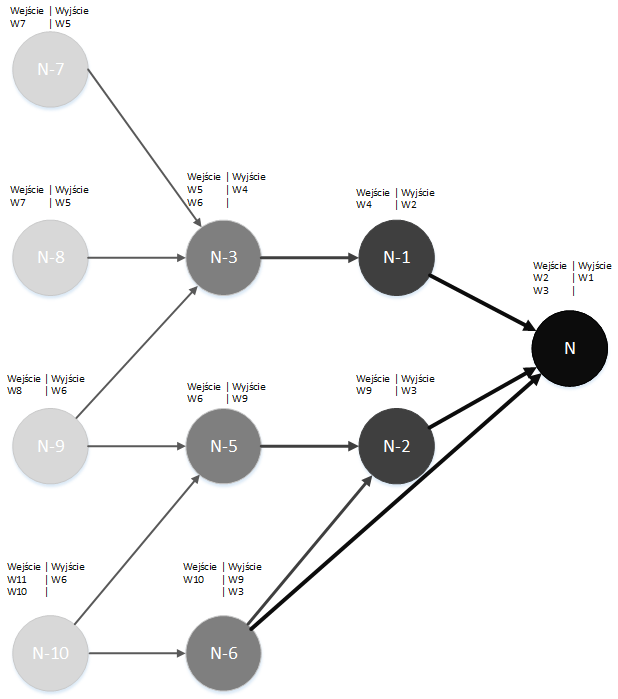
\includegraphics[width=1\linewidth]{pictures/visio/siec.png}
\caption{Przykładowy wycinek próbki sieci.}
\label{fig:siec}
\end{center}
\end{figure}

\begin{figure}[H]
\begin{center}
\centering
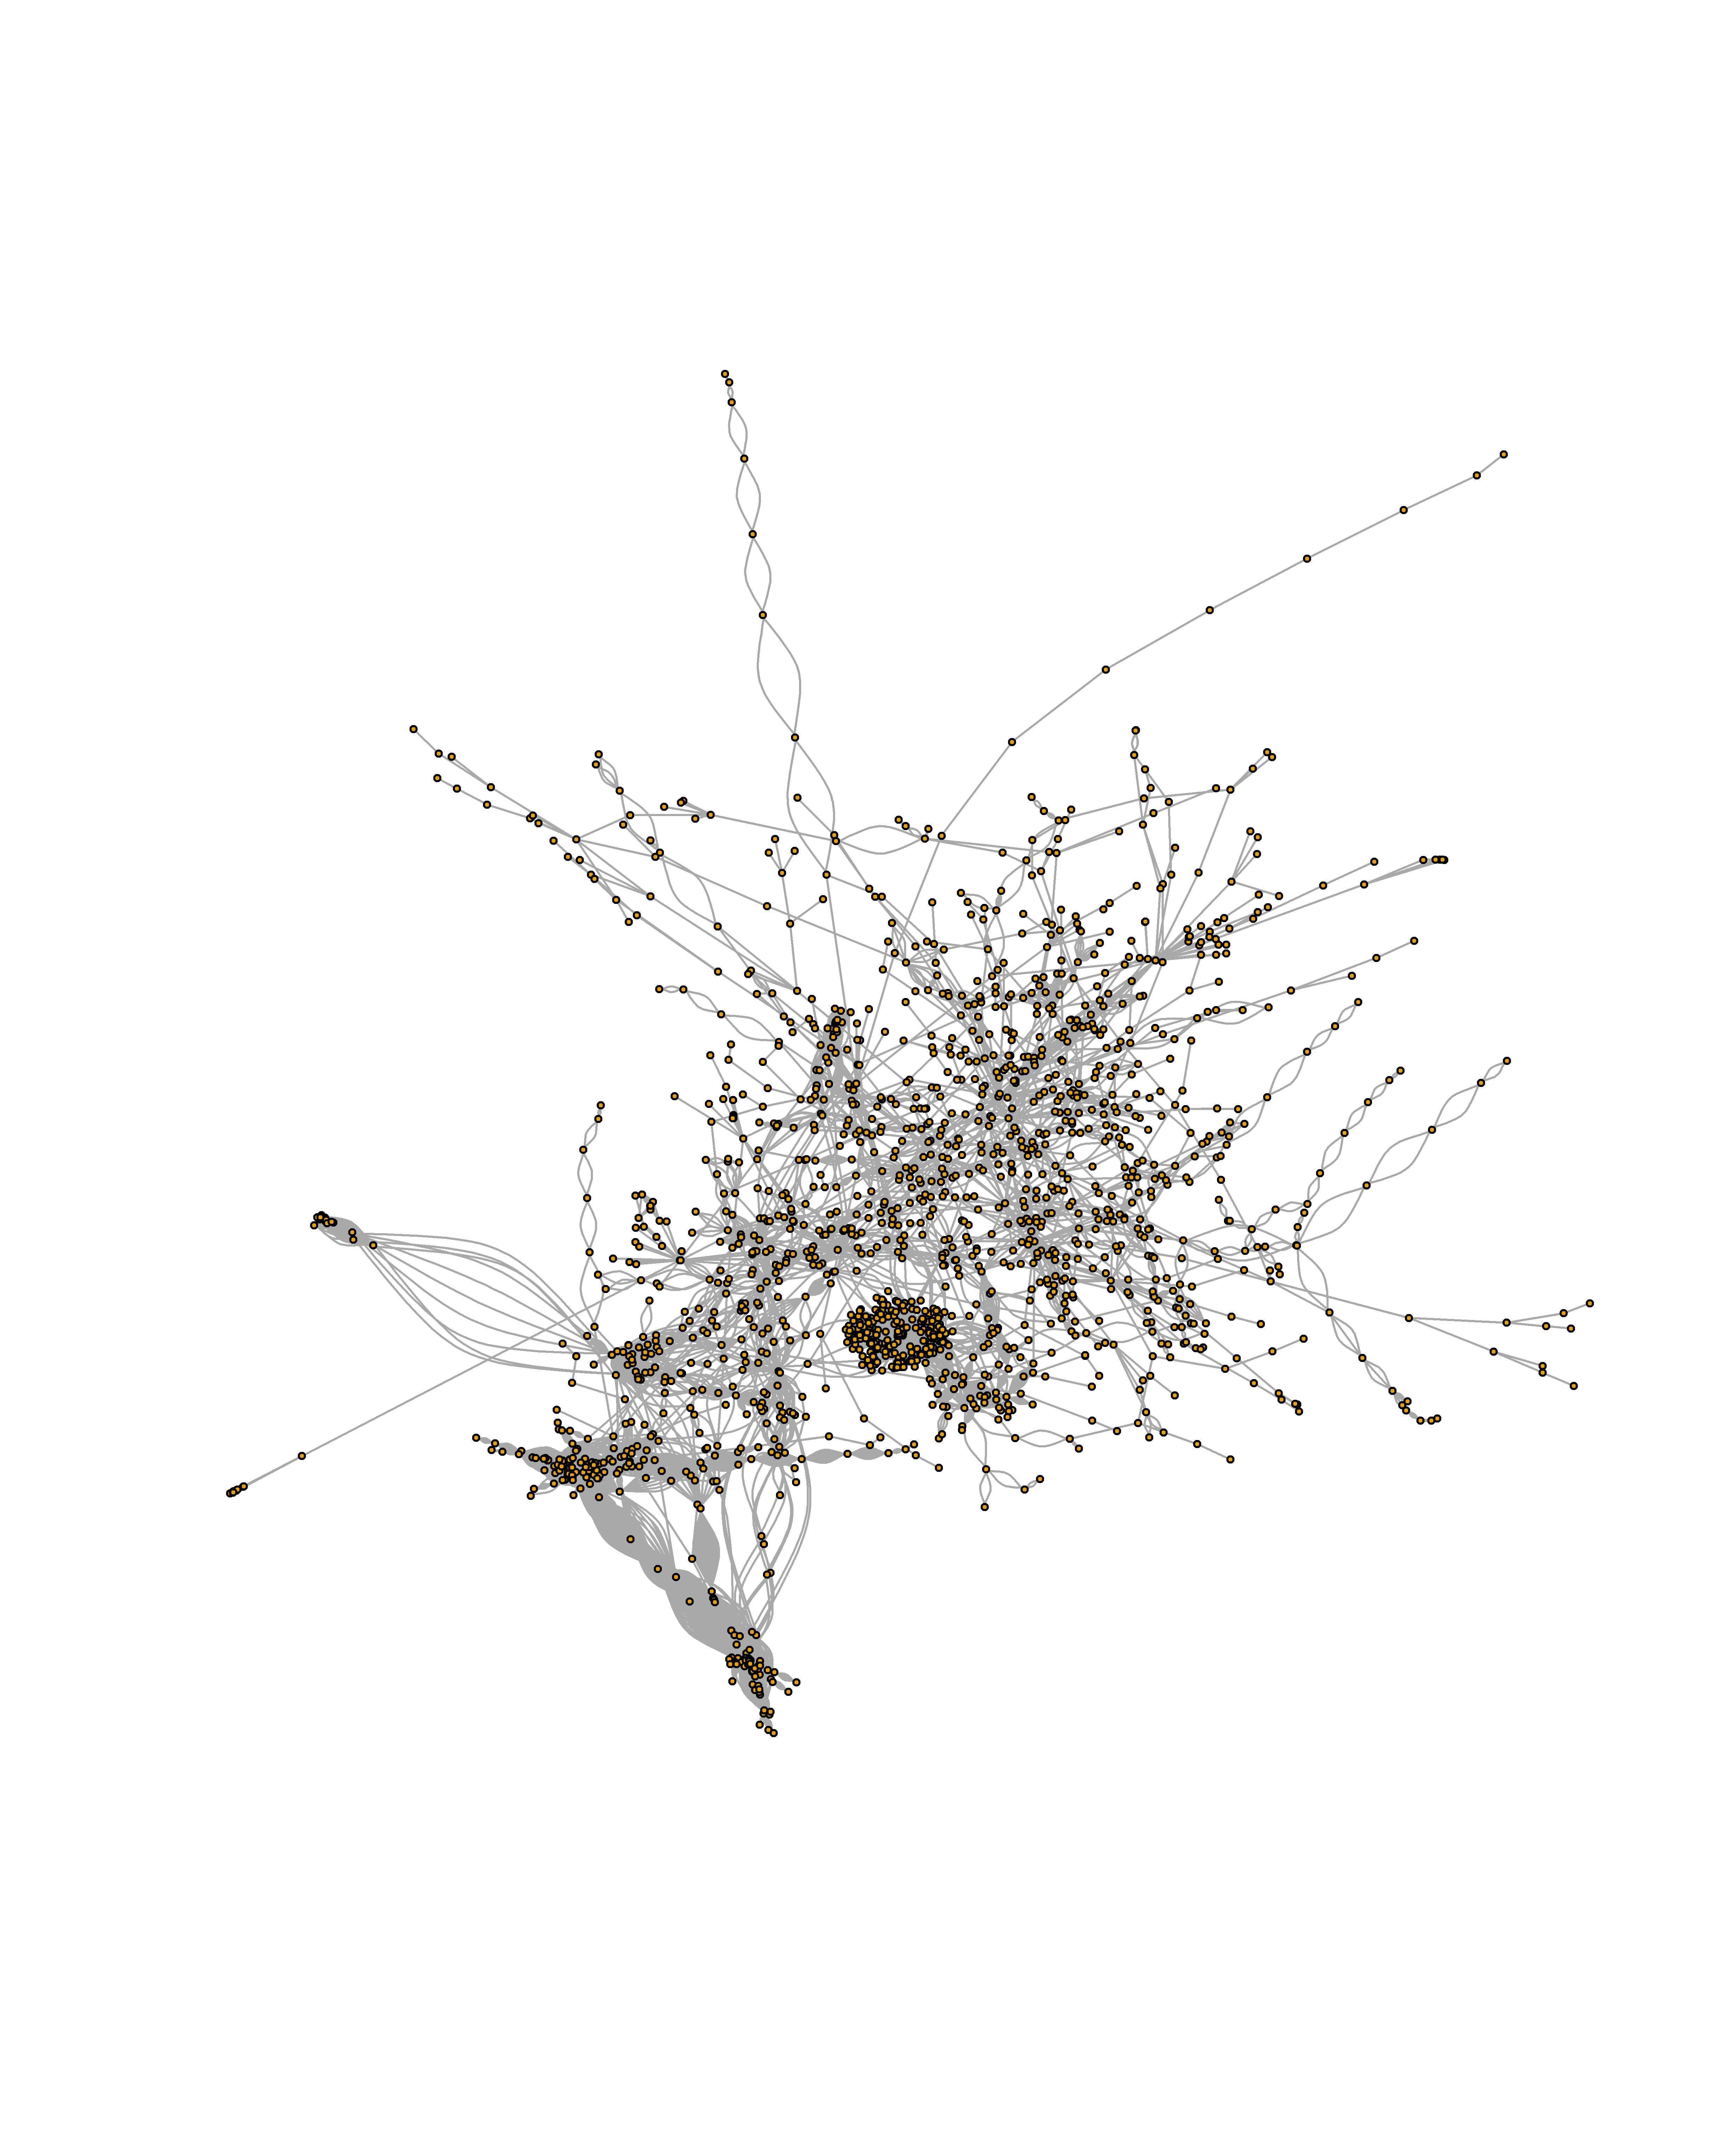
\includegraphics[width=1\linewidth]{pictures/graph/graph.png}
\caption{Wizualizacja grafu składającego się ze stu tysięcy połączeń.}
\label{fig:graf}
\end{center}
\end{figure}

\newpage
\indent Zastosowanie transakcji do stworzenia łańcucha transakcji pozwala na agregację wielu adresów w jeden komponent, który reprezentuje pojedynczy węzeł sieci. Taki sposób budowy sieci  daje możliwość szybszego wyszukiwania połączonych transakcji oraz możliwość efektywnego badania jej właściwości. Zauważyć jednak należy, że wybrane rozwiązanie próbkowania sieci nie jest jedyną możliwą metodą jej konstruowania. Przykładowo, rejestr bloków, który stanowi jeden z podstawowych mechanizmów zabezpieczania kryptowaluty Bitcoin, rozumiany być może jako sieć. Innym przykładem może być zastosowanie adresów zawartych w~transakcjach, jako pojedynczych węzłów sieci, które poprzez transakcje łączone są krawędziami. Takie podejście wymaga badania właściwości podstawowej jednostki na najniższym możliwym poziomie w sieci~Bitcoin, co jest bardzo czasochłonne i~ kosztowne. Metoda tworzenia sieci zastosowana w niniejszej pracy gwarantuje globalne spojrzenie na opisywany problem badawczy. 

\indent Przeprowadzone badania podzielono na dwie grupy pod względem reprezentowanych cech sieci. Pierwsza grupa reprezentuje analizę sieci przy pomocy algorytmów generycznych dla sieci złożonych. Algorytmy te nie są związane z problematyką fachową sieci, jednakże pozwalają na zbadanie podstawowych własności każdej z sieci. W~ramach analizy dla każdej próbki zbadano:
\begin{itemize}
\item[--] średnicę sieci,
\item[--] średnią długość ścieżek,
\item[--] średni stopień węzłów,
\item[--] średnią centralność węzłów.
\end{itemize}
Druga grupa przeprowadzonych badań pozwoliła na analizę sieci pod kątem jej specyficznych własności, które są bardzo mocno związane z jej problematyką. W ramach analizy dla każdej próbki zbadano:
\begin{itemize}
\item[--] średnią wartość transakcji,
\item[--] liczbę bloków potrzebnych do stworzenia próbki,
\item[--] średnią różnicę czasów kolejnych transakcji,
\item[--] różnice czasu granicznych transakcji.
\end{itemize}

\indent Badania z grupy pierwszej przeprowadzono przy pomocy biblioteki \textit{Igraph}, natomiast algorytmy potrzebne do przeprowadzenia badań z grupy drugiej zostały przygotowane samodzielnie.

\section{Eksperyment}
W ramach przeprowadzonych badań dla każdej z metryk stworzono mapę cieplną przedstawiającą wartości poszczególnych właściwości sieci. Na wykresie zaprezentowano również średnią wartość dla każdego z okresu wraz z odchyleniem standardowym, z którego stworzono regresję liniową. Na podstawie tych danych przeprowadzono analizę oraz określono trend zmian w sieci. Pierwsze cztery analizy przeprowadzono dla właściwości sieci niebezpośrednio powiązanych z typem sieci. Kolejne cztery przeprowadzone analizy związane są wyłącznie z fachowością badanej sieci.

\subsection{Badanie średnicy sieci}
\label{srednica_sieci}
\indent Średnica sieci jest długością 
\begin{equation}
\label{eq:srednica_sieci}
	max_{u,v}d(u,v)
\end{equation}
najdłuższej ścieżki znalezionej wśród najkrótszych ścieżek pomiędzy dwoma którymikolwiek węzłami sieci $(u,v)$, gdzie $d(u,v)$ jest długością grafu\cite{barabasi2016network}. Długość grafu jest minimalną długością ścieżki (stworzonej z węzłów) potrzebnej do połączenia dwóch określonych węzłów. Inaczej mówiąc średnica grafu jest maksymalną ilością węzłów, jakie trzeba pokonać by przejść z jednego węzła do drugiego.

\indent Dla badanej sieci oznacza to maksymalną ścieżkę połączonych transakcji, a co za tym idzie, maksymalną krotność przekazywania pomiędzy adresami publicznymi bitcoinów. Na podstawie wartości długości ścieżki można wnioskować o własnościach sieci, takich jak na przykład jej gęstości.

\indent Na rysunku~\ref{fig:s1} przedstawiono mapę ciepła średnicy sieci dla każdej z próbek. Na jej podstawie można wnioskować, że dla większości przypadków próbki w poszczególnych okresach są zbliżone. Zaobserwować można również, że w każdym z okresów istnieją pojedyncze sieci mocno odbiegające od reszty. Jedną z tych anomalii jest średnica sieci dla próbki zaczynającej się od transakcji szóstej, która została zrealizowana \textit{2017-03-31}. Istnieje prawdopodobieństwo, że jest to transakcja realizowana w ramach wielokrotnego przesyłania bitcoinów przez jednego właściciela pomiędzy własnymi adresami w celu próby ukrycia ich źródła.

\indent Na wykresie~\ref{fig:s2} przedstawiono regresję liniową na podstawie średniej średnicy dla okresu z odchyleniem standardowym. Z~wykresu wynika, że gęstość sieci rośnie w czasie, o czy świadczy trend spadkowy średnicy sieci. Wzrost gęstości oznacza, że w sieci występuje coraz więcej krawędzi w stosunku do ilości węzłów. Dla sieci Bitcoin wzrost gęstości sieci oznacza wzrost ilość transakcji realizowanych na pojedyncze adresy publiczne, w~krótszym czasie. Można zatem wnioskować, że bitcoiny coraz częściej gromadzone są na pojedynczych adresach. Odchylenia standardowe widoczne na~\ref{fig:s2} wynikają z pojedynczych próbek mocno odbiegających od średniej. Odrzucenie próbek (najwyżej oraz najniżej wartościowanych) z każdego okresu zniwelowałoby znacząco rozpiętość odchylenia standardowego. Przykładem może być wcześniej omawiana próbka zaczynająca się od transakcji $T6$ z okresu \textit{2017-03-31}. 

\newpage
\begin{figure}[H]
\centering
  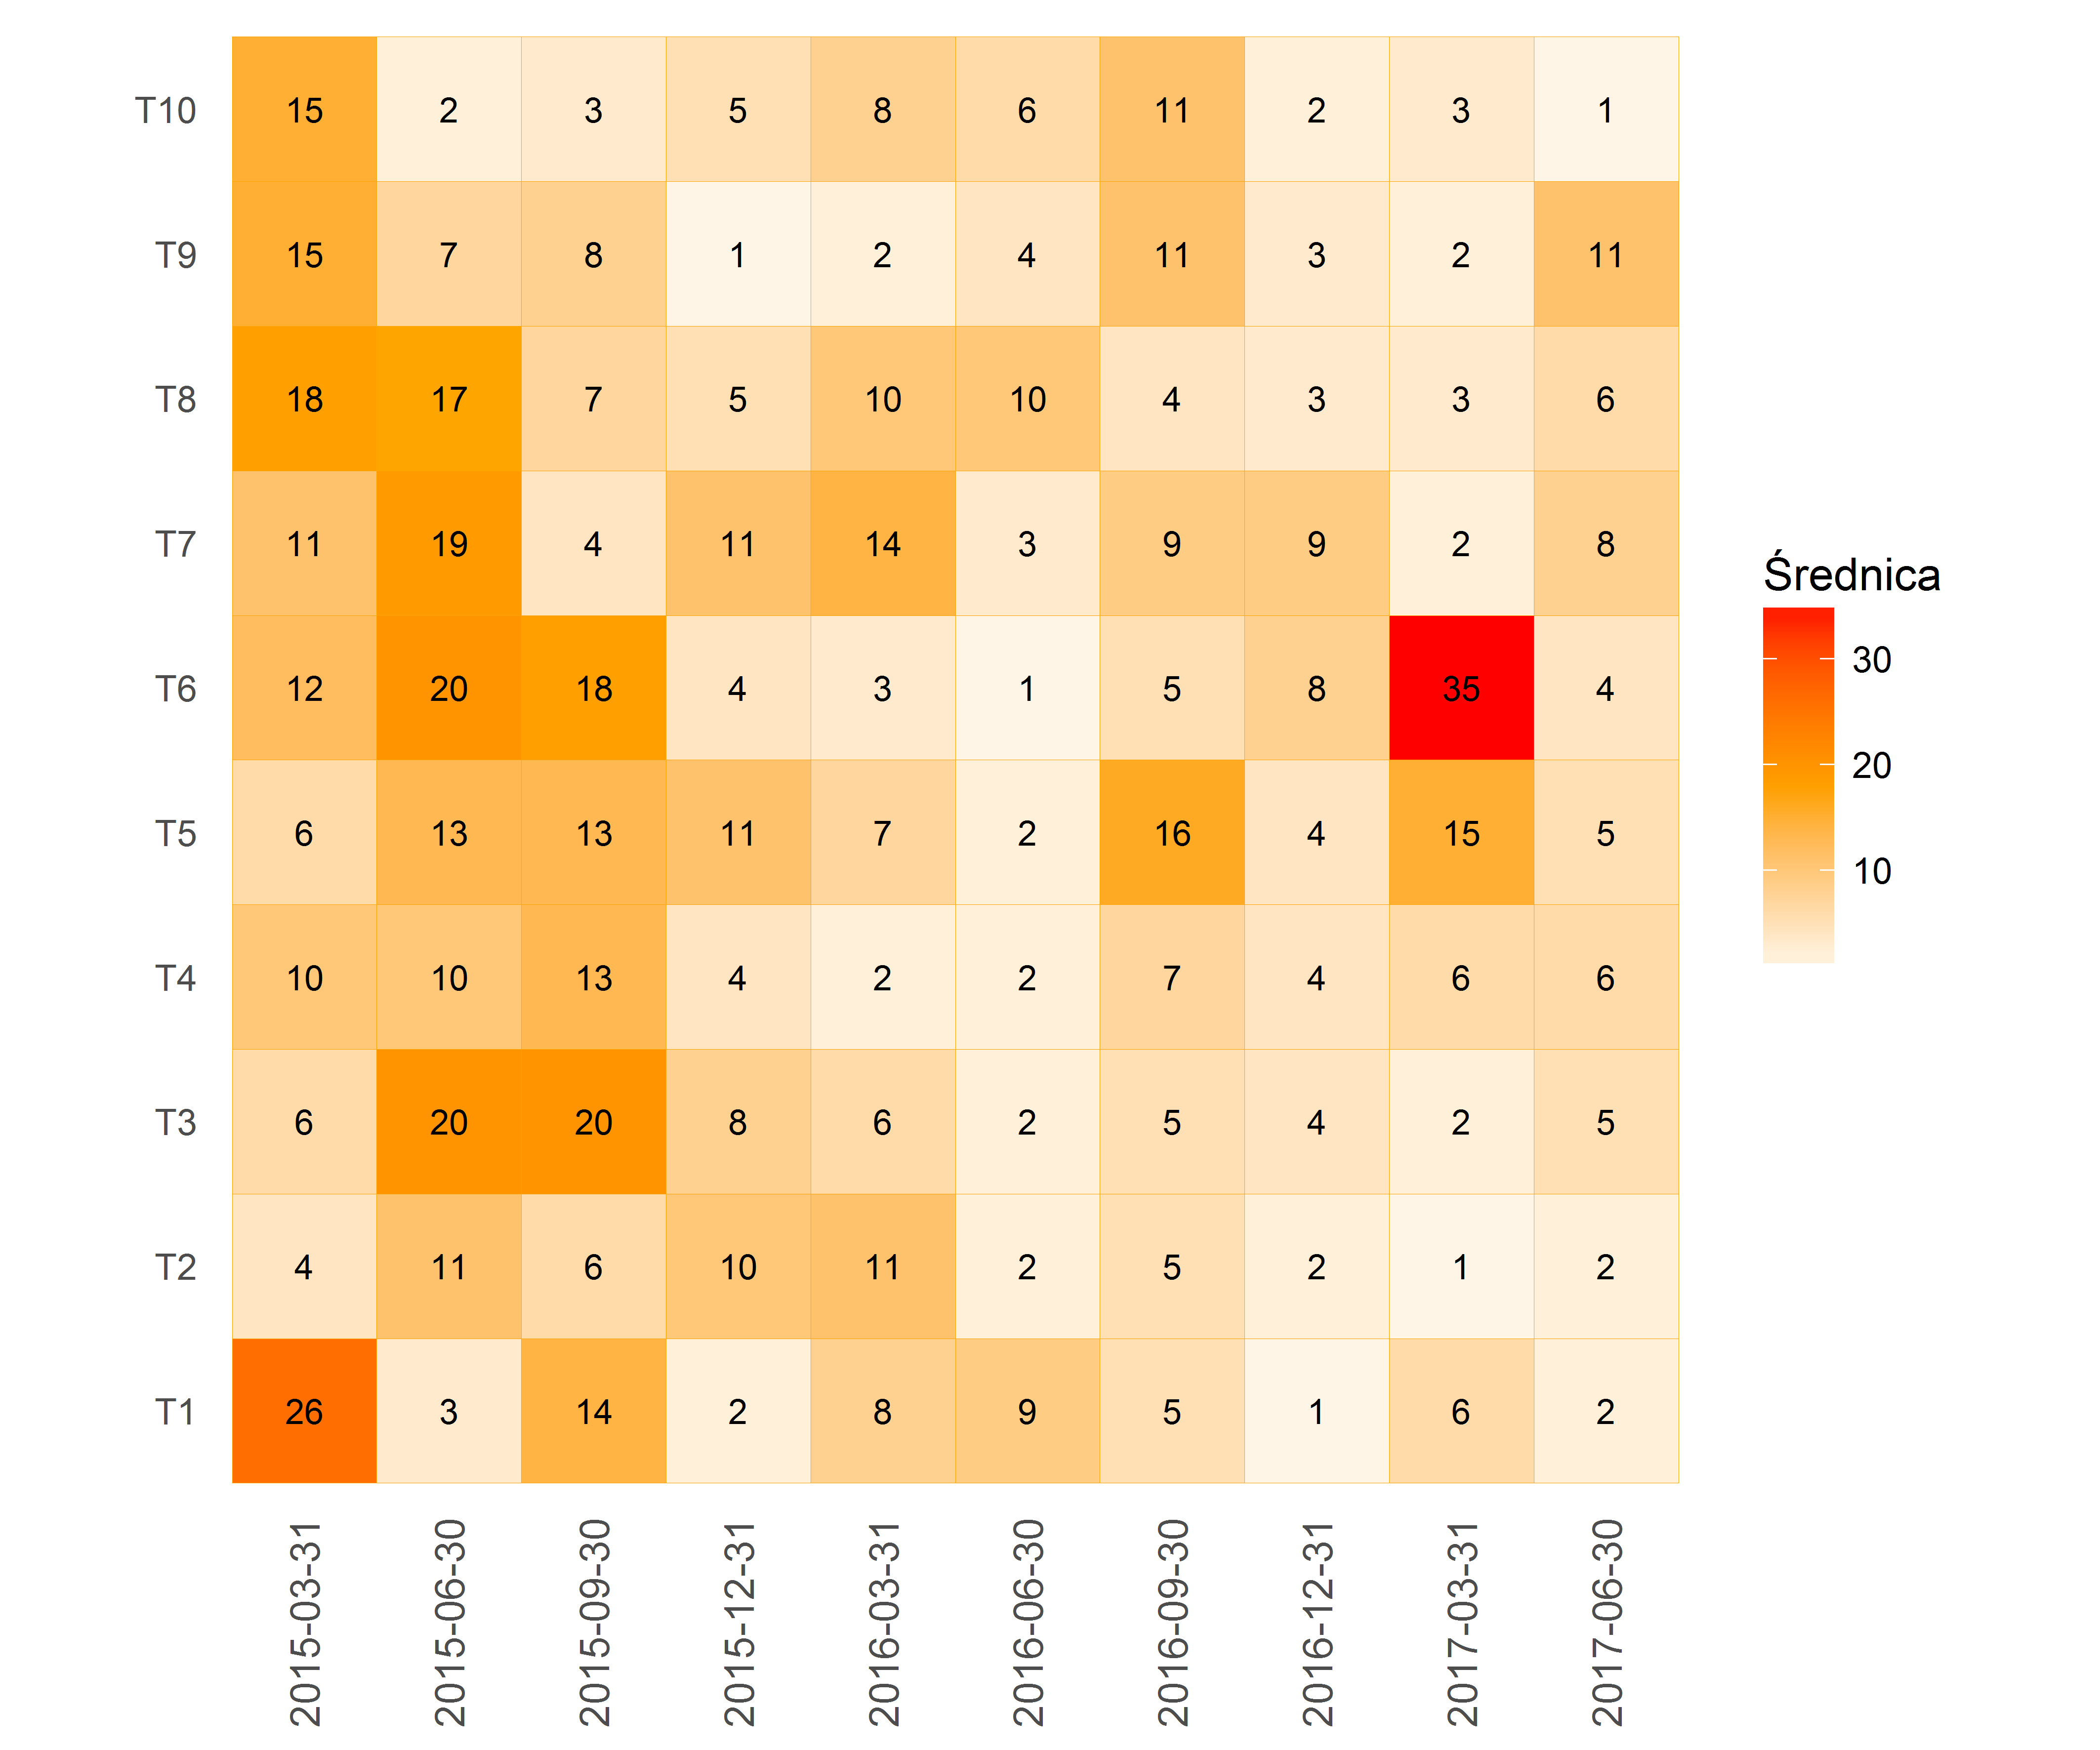
\includegraphics[width=\chartsWidth\linewidth]{pictures/srednica/srednica_hm.png}
  \caption{Mapa cieplna średnicy sieci dla 10 prób w 10 okresach.}
  \label{fig:s1} 
\end{figure}
\begin{figure}[H]
\centering
  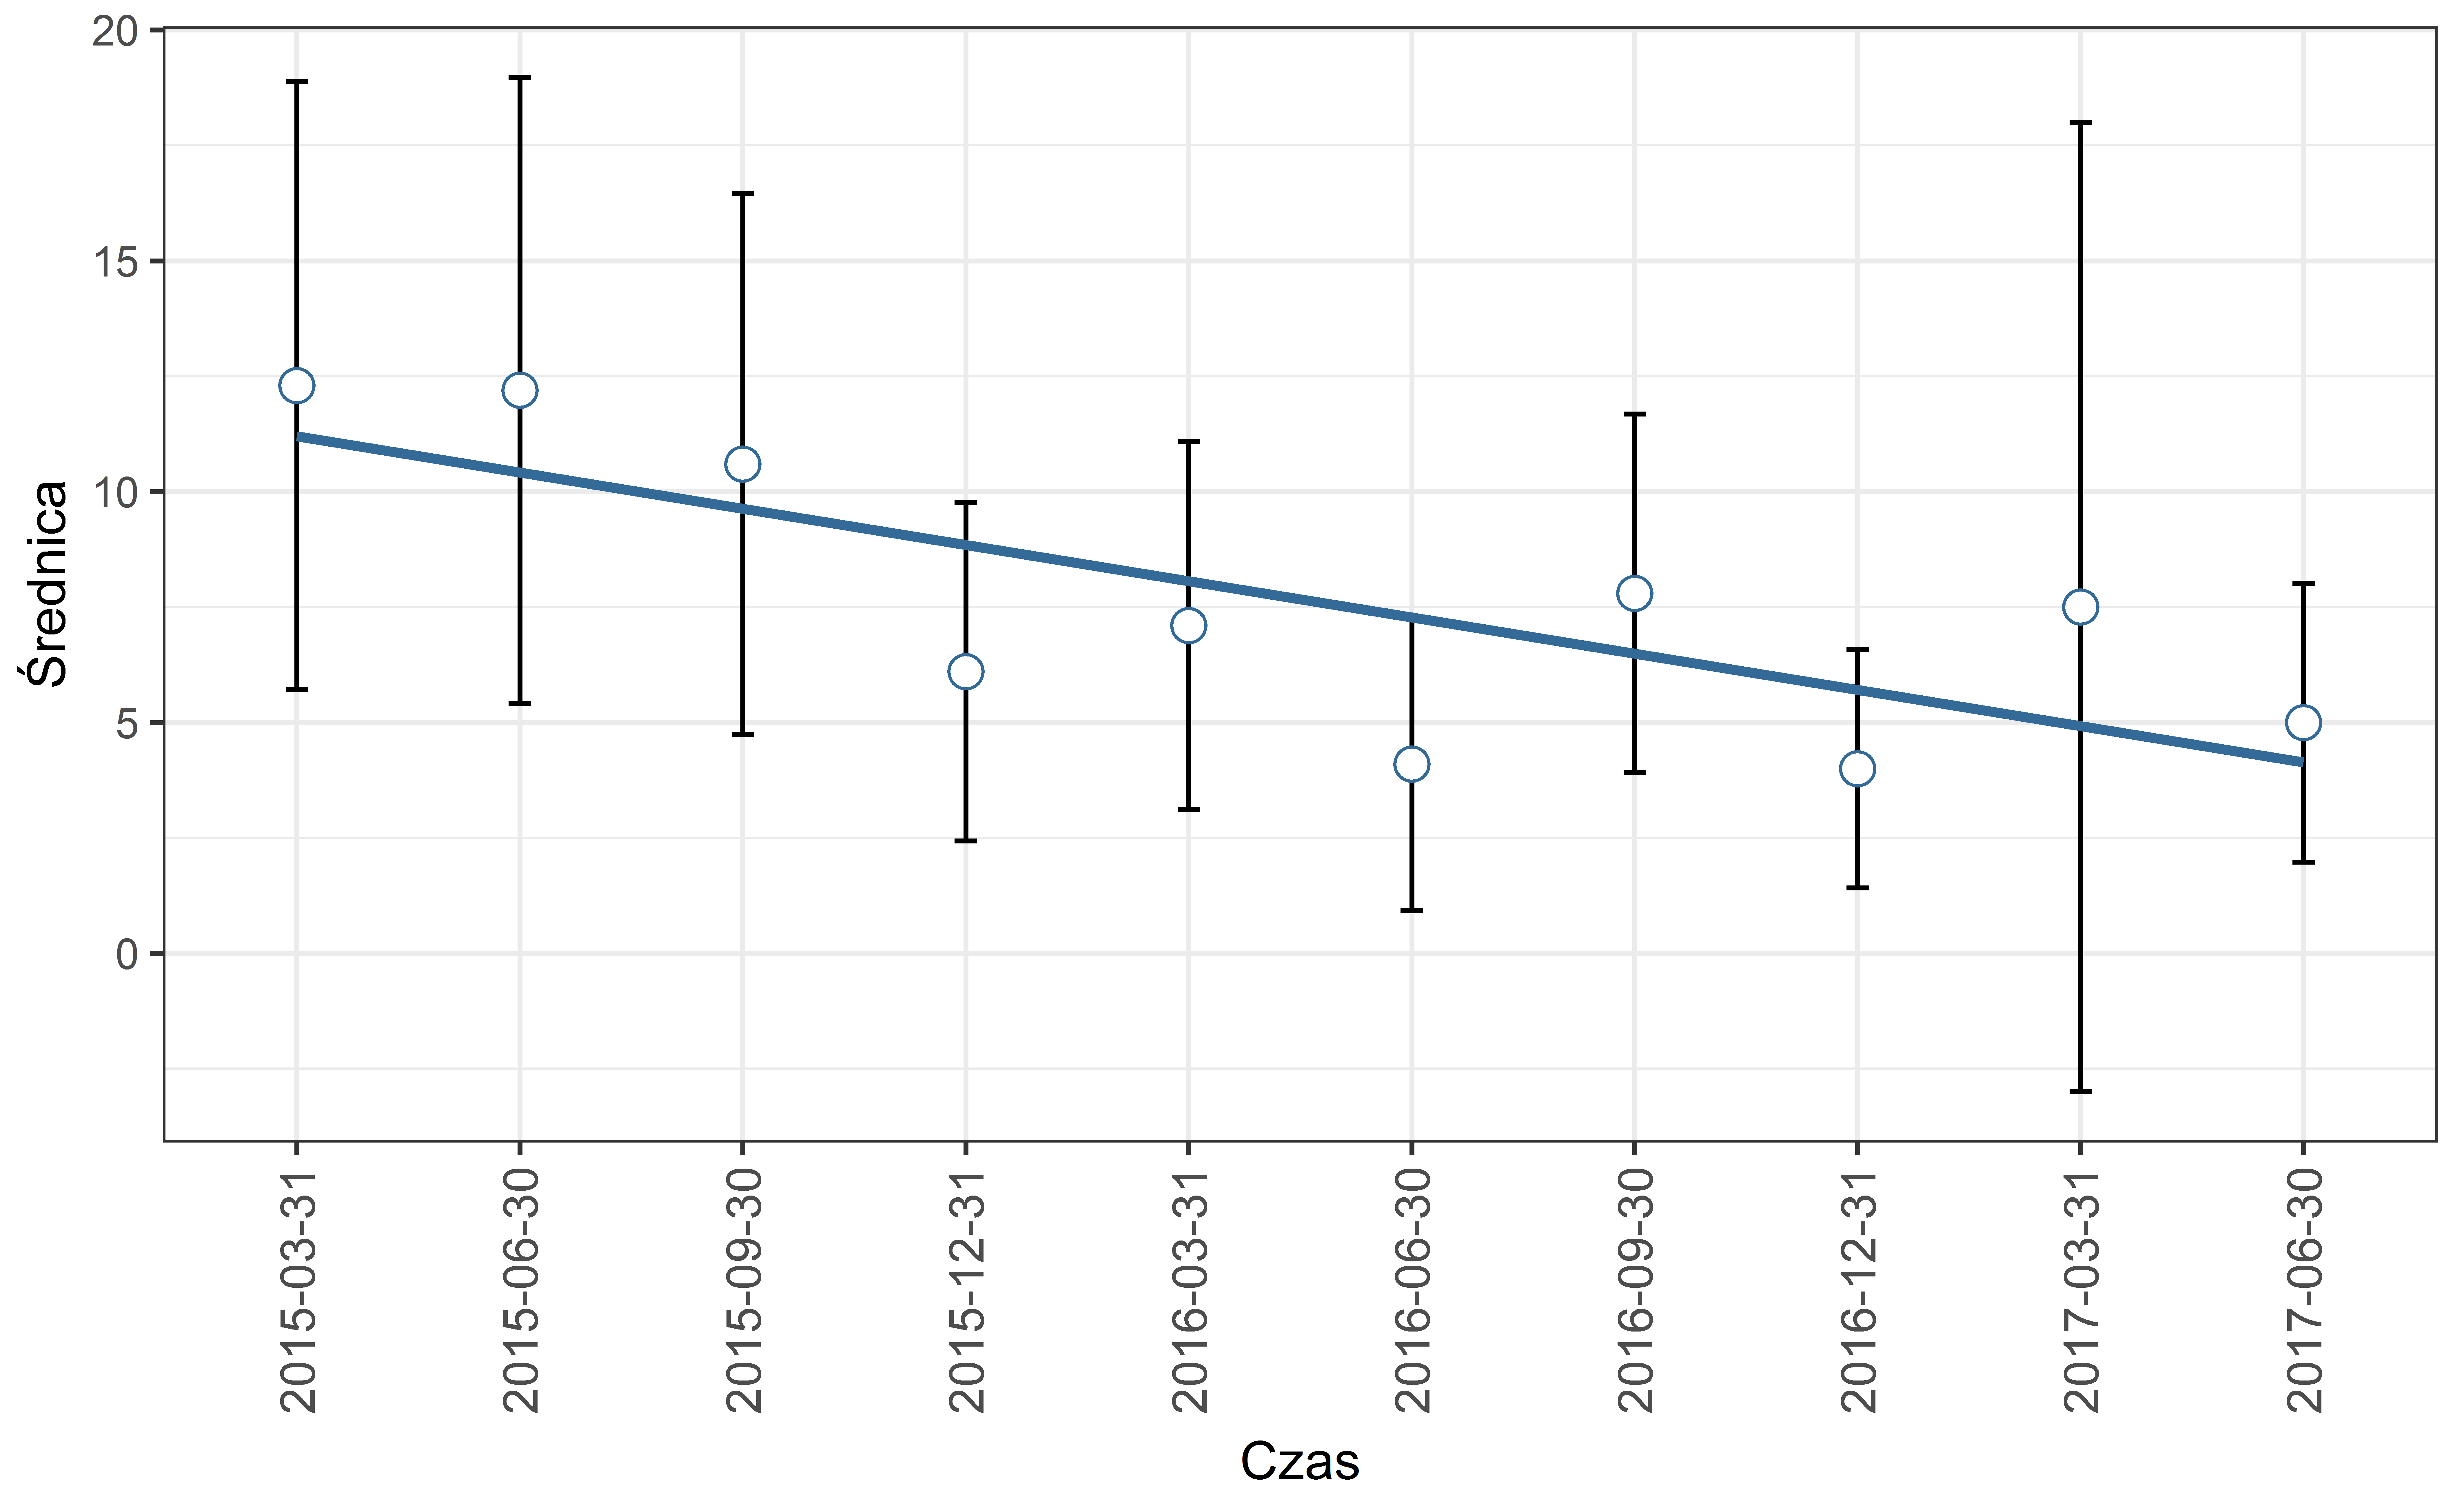
\includegraphics[width=\chartsWidth\linewidth]{pictures/srednica/srednica_sda.png}
  \caption{Regresja liniowa średniej średnicy sieci dla 10 okresów z odchyleniem standardowym.}
  \label{fig:s2}
\end{figure}


\newpage
\subsection{Badanie średniej długość ścieżki}
\label{dlugosc_sciezki}
\indent Średnia długość ścieżki w sieci jest średnią wartością 
\begin{equation}
\label{eq:dlugosc_sciezki}
	\sum_{i \ne j}^{} d(u_i,v_j)\frac{1}{n(n-1)}
\end{equation}
wszystkich możliwych par węzłów $(u_j,v_j)$ w grafie, gdzie $d(u_i,v_j)$ jest najkrótszą długością ścieżki pomiędzy węzłami $(u_i,v_j)$, a $n$ jest ilością węzłów\cite{wasserman1994social}. Długość ścieżki została zdefiniowana w~\ref{srednica_sieci}. 

\indent Sieć Bitcoin jest siecią skierowaną, a każda z transakcji posiada niepowtarzalny adres. Eliminuje to możliwość pojawienia się cyklu w grafie, dlatego też ilość możliwych ścieżek w analizowanej sieci jest ograniczona. W badanej sieci średnia długość ścieżki oznacza średnią ilość transakcji, przy pomocy których przekazywano kolejno bitcoiny.

\indent Na podstawie mapy cieplnej~\ref{fig:sds1} reprezentującej średnią długość ścieżki dla prób zaobserwowano pojedyncze przypadki odchyleń wartości badanej cechy. W przypadku transakcji szóstej zrealizowanej \textit{2017-03-31}, przyczyna prawdopodobnie jest analogiczna do przypadku analizy średnicy sieci, tzn. wielokrotne przesyłanie środków jednej osoby przez wiele adresów publicznych w~sieci.

\indent Na wykresie~\ref{fig:sds2} reprezentującym regresję liniową średniej wartości długości sieci z~okresów zaobserwowano trend spadkowy. W przypadku badanych próbek średnia długość sieci zmienia się analogicznie do jej średnicy. Determinuje to zmniejszającą się średnią liczbę kolejnych transakcji w badanych próbach. Może to oznaczać coraz większą ilość transakcji rejestrowanych w~sieci. Potwierdza to wzrastającą gęstość sieci.

\indent Można przypuścić, że uszczegółowienie informacji dotyczących przypadków znaczących odchyleń standardowych poprzez wykonanie dodatkowych badań pozwoliłoby jednoznacznie stwierdzić ich przyczynę. Jednakże istnieje prawdopodobieństwo, że właściwości sieci nie są stałe w jednym okresie czasu, a zmieniają się dynamicznie w~zależności od aktywności poszczególnych uczestników sieci.

\newpage
\begin{figure}[H]
\centering
  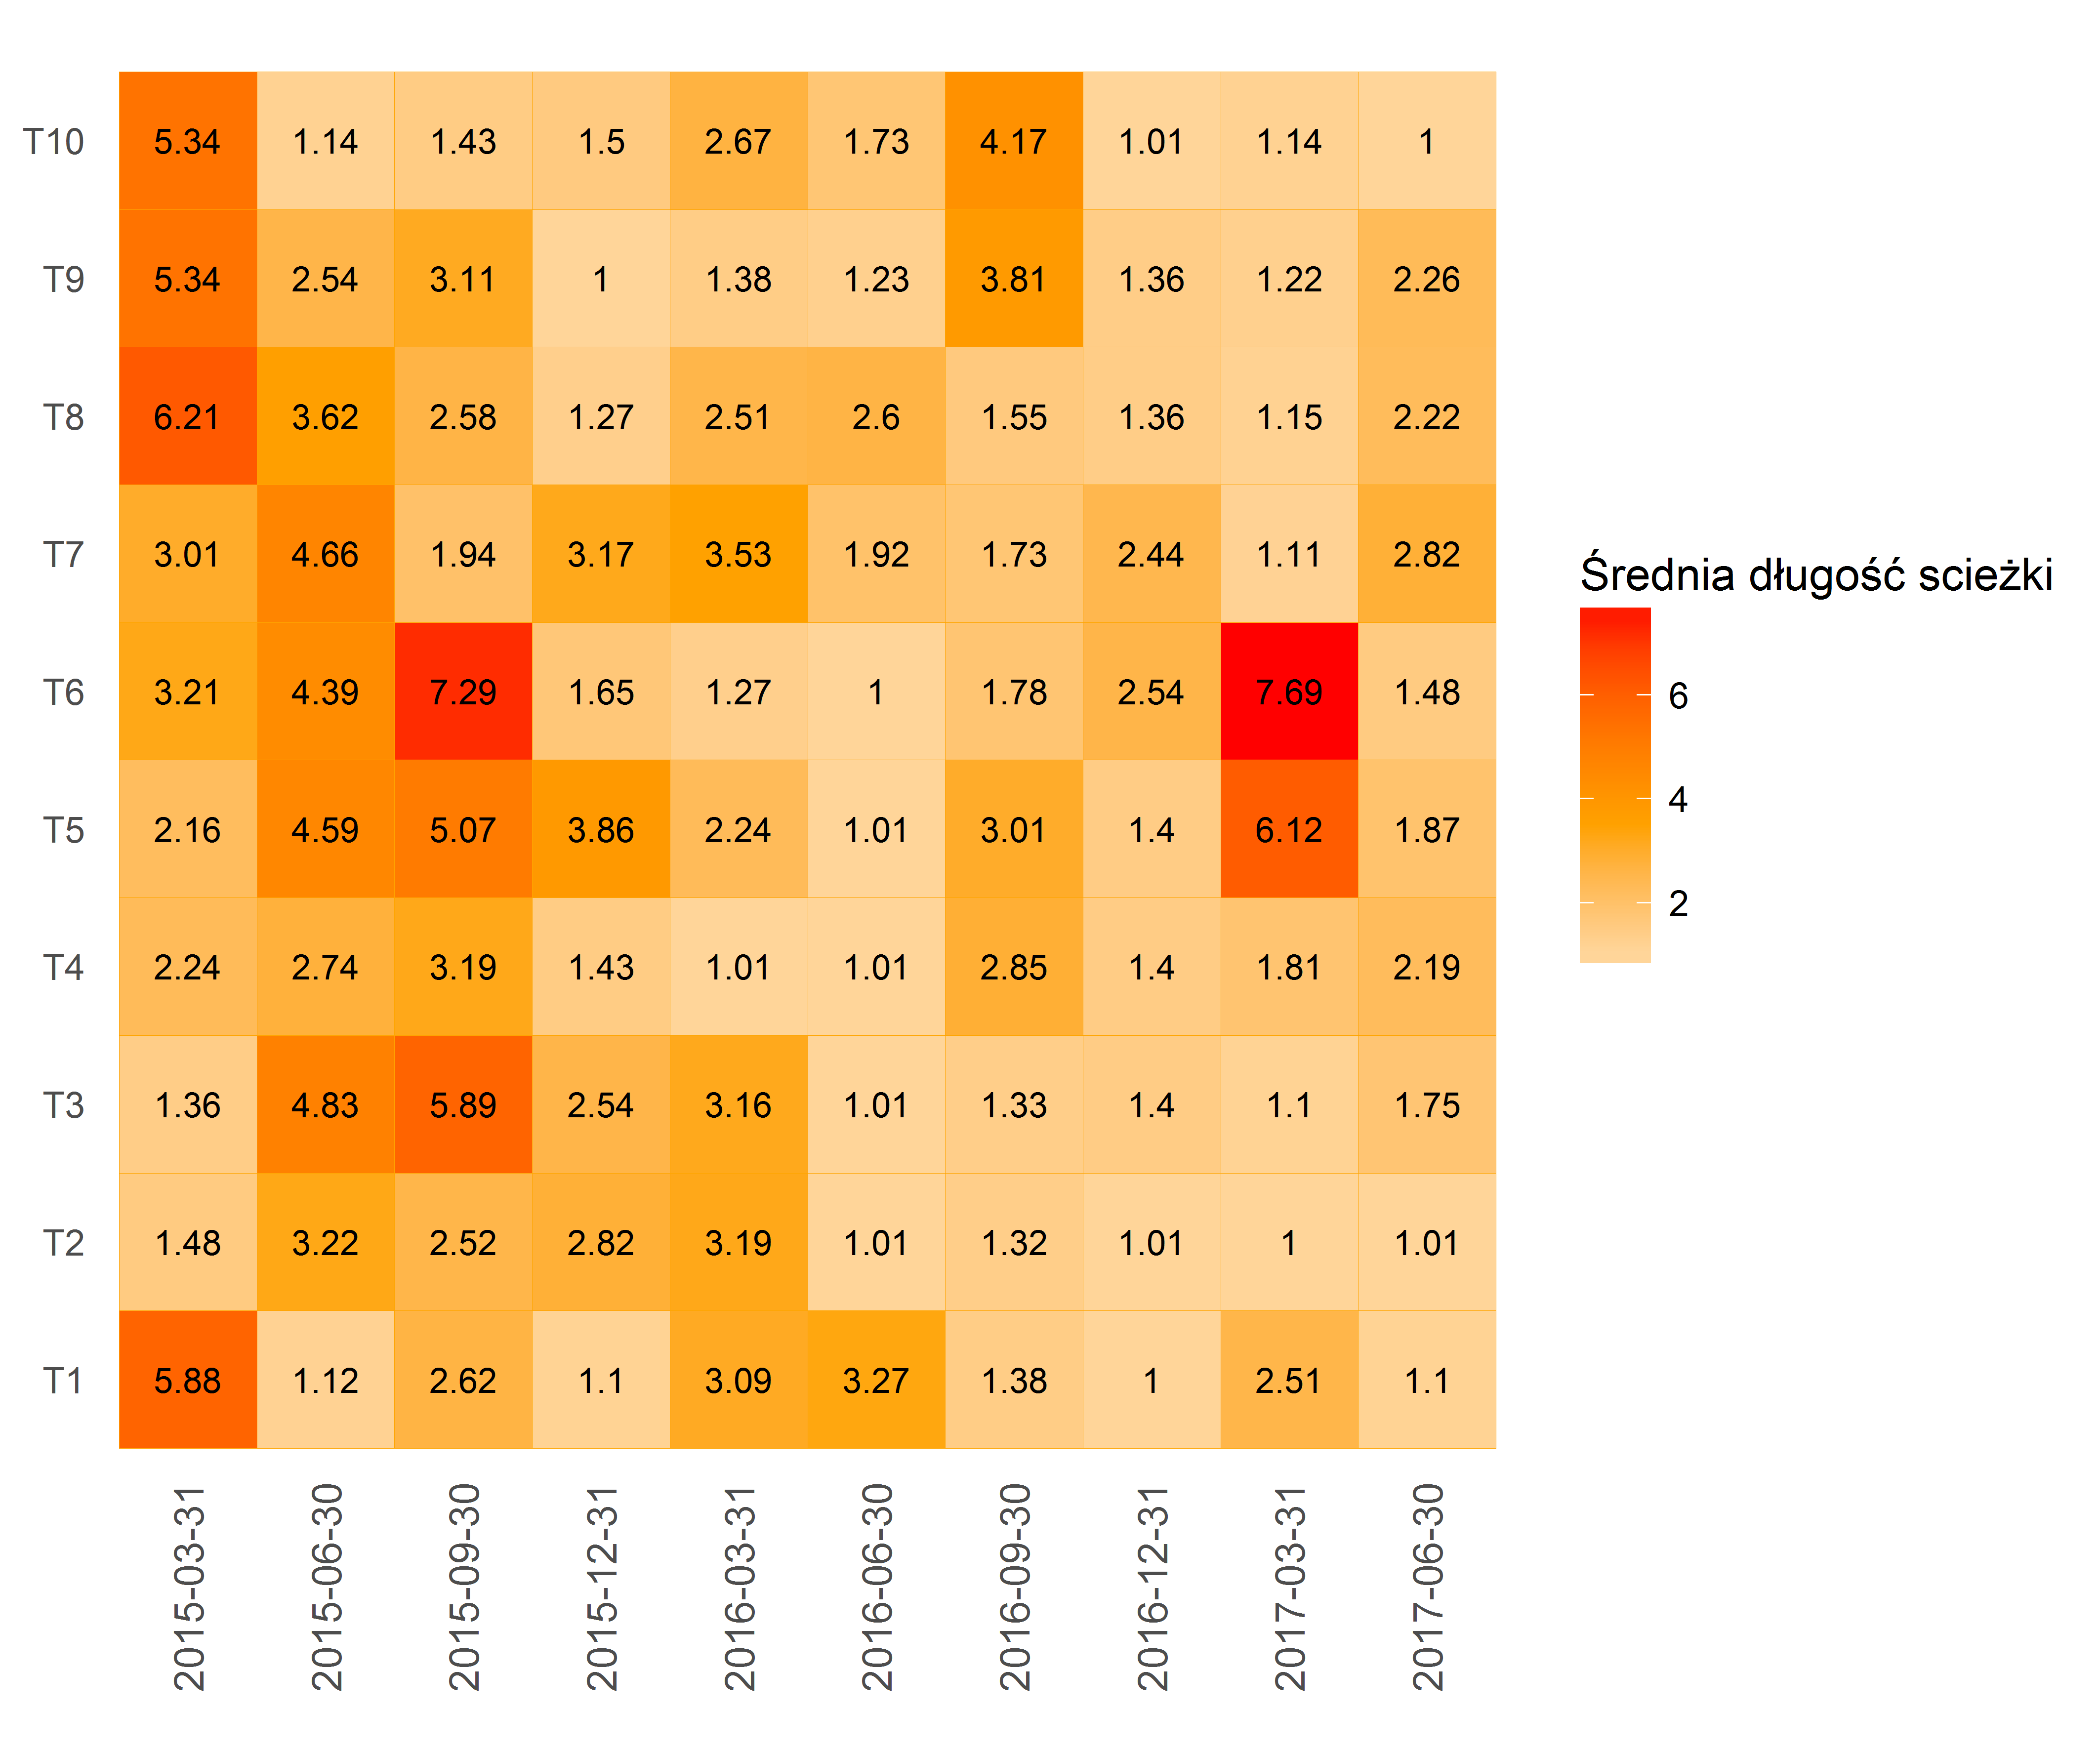
\includegraphics[width=\chartsWidth\linewidth]{pictures/srednia_dlugosc_sciezki/srednia_dlugosc_sciezki_hm.png}
  \caption{Mapa cieplna średniej długości scieżki w sieci dla 10 prób w 10 okresach.}
  \label{fig:sds1}
\end{figure}
\begin{figure}[H]
\centering
  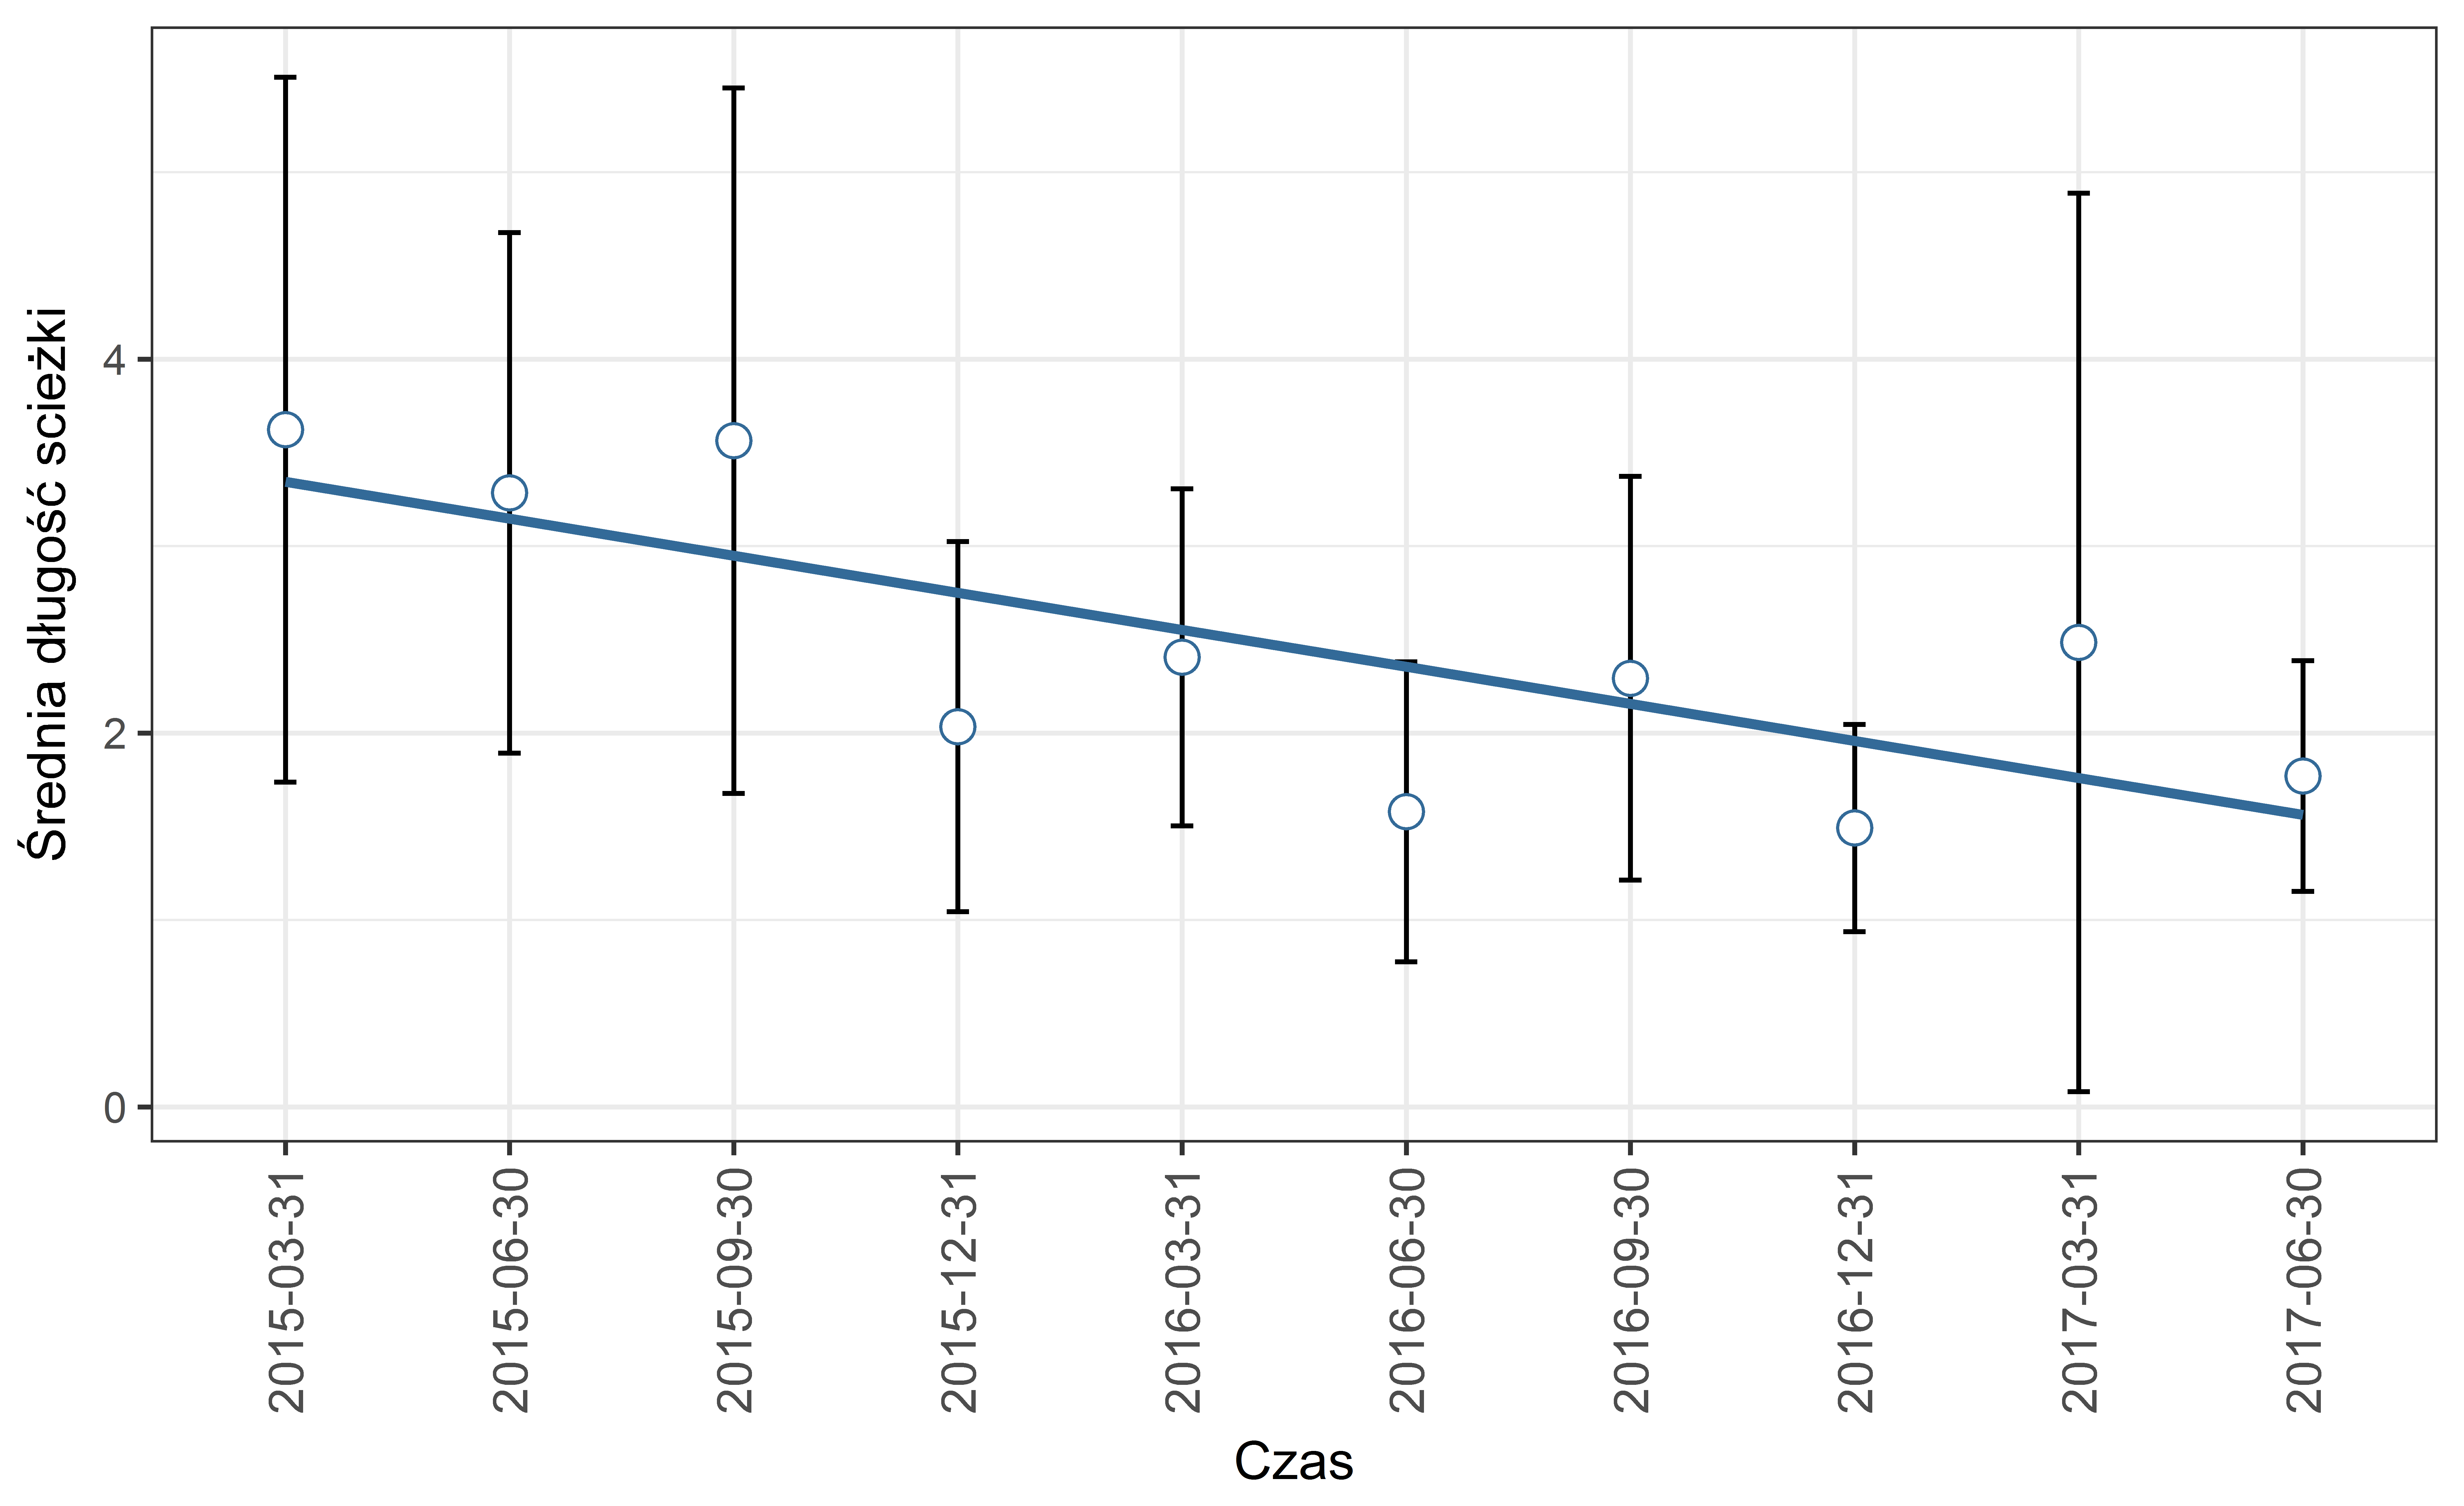
\includegraphics[width=\chartsWidth\linewidth]{pictures/srednia_dlugosc_sciezki/srednia_dlugosc_sciezki_sda.png}
  \caption{Regresja liniowa średniej długości scieżki sieci dla 10 okresów z odchyleniem standardowym.}
  \label{fig:sds2}
\end{figure}

\newpage
\subsection{Badanie średniego stopnia węzła}
\label{stopien_wezla}
\indent Stopień węzła $v$ grafu oznacza liczbę krawędzi w grafie, które bezpośrednio dotykają węzła~$v$. W grafach skierowanych wyróżnia się wejściowy stopień węzła (ilość krawędzi skierowanych w stronę węzła) oraz wyjściowy stopień węzła (ilość krawędzi skierowanych od strony węzła). Suma wejściowego stopnia węzła oraz wyjściowego stopnia węzła daje wynikowy stopień węzła. Średni stopień węzła obliczany jest jako 
\begin{equation}
\label{eq:stopien_wezla}
  \frac{\sum_i^n\deg(v_i)}{n}
\end{equation} 
gdzie $deg(v_i)$ to stopień i-tego węzła, a $n$ to ilość węzłów\cite{barabasi2016network}. W~celu zminimalizowania ryzyka popełnienia błędu, podczas interpretacji obliczanej średniej, badana próba powinna mieć rozkład normalny. W przeciwnym przypadku należy przedstawić dodatkowe źródło informacji o~próbie, które zobrazuje częstotliwość występowania poszczególnych wartości, np. histogram. 

\indent W trakcie budowania sieci procesowanie każdej pojedynczej transakcji polega na sprawdzeniu jej adresów wyjściowych z adresami wejściowymi każdej transakcji do tej pory dołączonej do sieci. Wykrycie tego samego adresu w tych dwóch zbiorach adresów transakcji powoduje powstanie krawędzi, która je łączy. W przypadku badania stopnia węzła transakcji w łańcuchu transakcji sieci Bitcoin określana jest ilość transakcji, z którymi dana transakcja dzieli adresy w danej próbce. Średni stopień węzła w próbce oznacza średnią ilość transakcji, z którymi połączona jest każda transakcja w próbce. 

\indent Na podstawie mapy cieplnej~\ref{fig:sw1} badanej właściwości wywnioskowano, że średnia ilość transakcji, z którymi połączona jest każda transakcja jest bardzo zróżnicowana. Wynika to z różnego poziomu aktywności właścicieli adresów biorących udział w~transakcjach w~danych okresach czasu oraz ilości nowych adresów generowanych przez uczestników sieci. Prezentowane wyniki można interpretować na trzy różne sposoby. Wysoka wartość średniego stopnia węzła może świadczyć o wzmożonej działalność właściciela adresu jako odbiorcy, czy jako nadawcy zleceń. Niska wartość średniego stopnia węzła nie wyklucza dużej aktywności pojedynczych klientów sieci, a oznaczać może dużą ilość nowo generowanych adresów, na które przekazywane były środki. Trzecią prawdopodobną sytuacją jest mało dynamiczny fragment sieci, w którym utworzono niewiele nowych adresów, a~środki przekazywane były kolejno pomiędzy ograniczoną ilości uczestników sieci.

\indent Znaczące zróżnicowania badanej cechy zaobserwowano również na wykresie~\ref{fig:sw2}, który przedstawia regresję liniową stworzoną na podstawie wartości średnich z odchyleniami standardowymi dla okresu. Wykres ten wskazuje na tendencję do wzrostu analizowanej własności, jednakże z powodów wskazanych w akapicie pierwszym oraz dużych odchyleń standardowych, zaobserwowanych na prezentowanych wykresach, postanowiono przeprowadzić dodatkową analizę.

\indent Na histogramie~\ref{fig:sw3} przedstawiono ilość wystąpień poszczególnych wartości stopni węzłów dla wszystkich próbek razem. Zauważono zdecydowaną dominację wartości na poziomie do tysiąca wchodzących i wychodzących transakcji. Wcześniej zauważone odchylenia standardowe wynikają z anomalii sięgających do 50 tysięcy połączonych transakcji, z~którymi dana transakcja dzieli adresy w danej próbce. Istnieje prawdopodobieństwo, że~transakcje, których stopień węzła mocno odbiega od dominanty są jednymi z kluczowych węzłów w sieci.

\begin{figure}[H]
\centering
   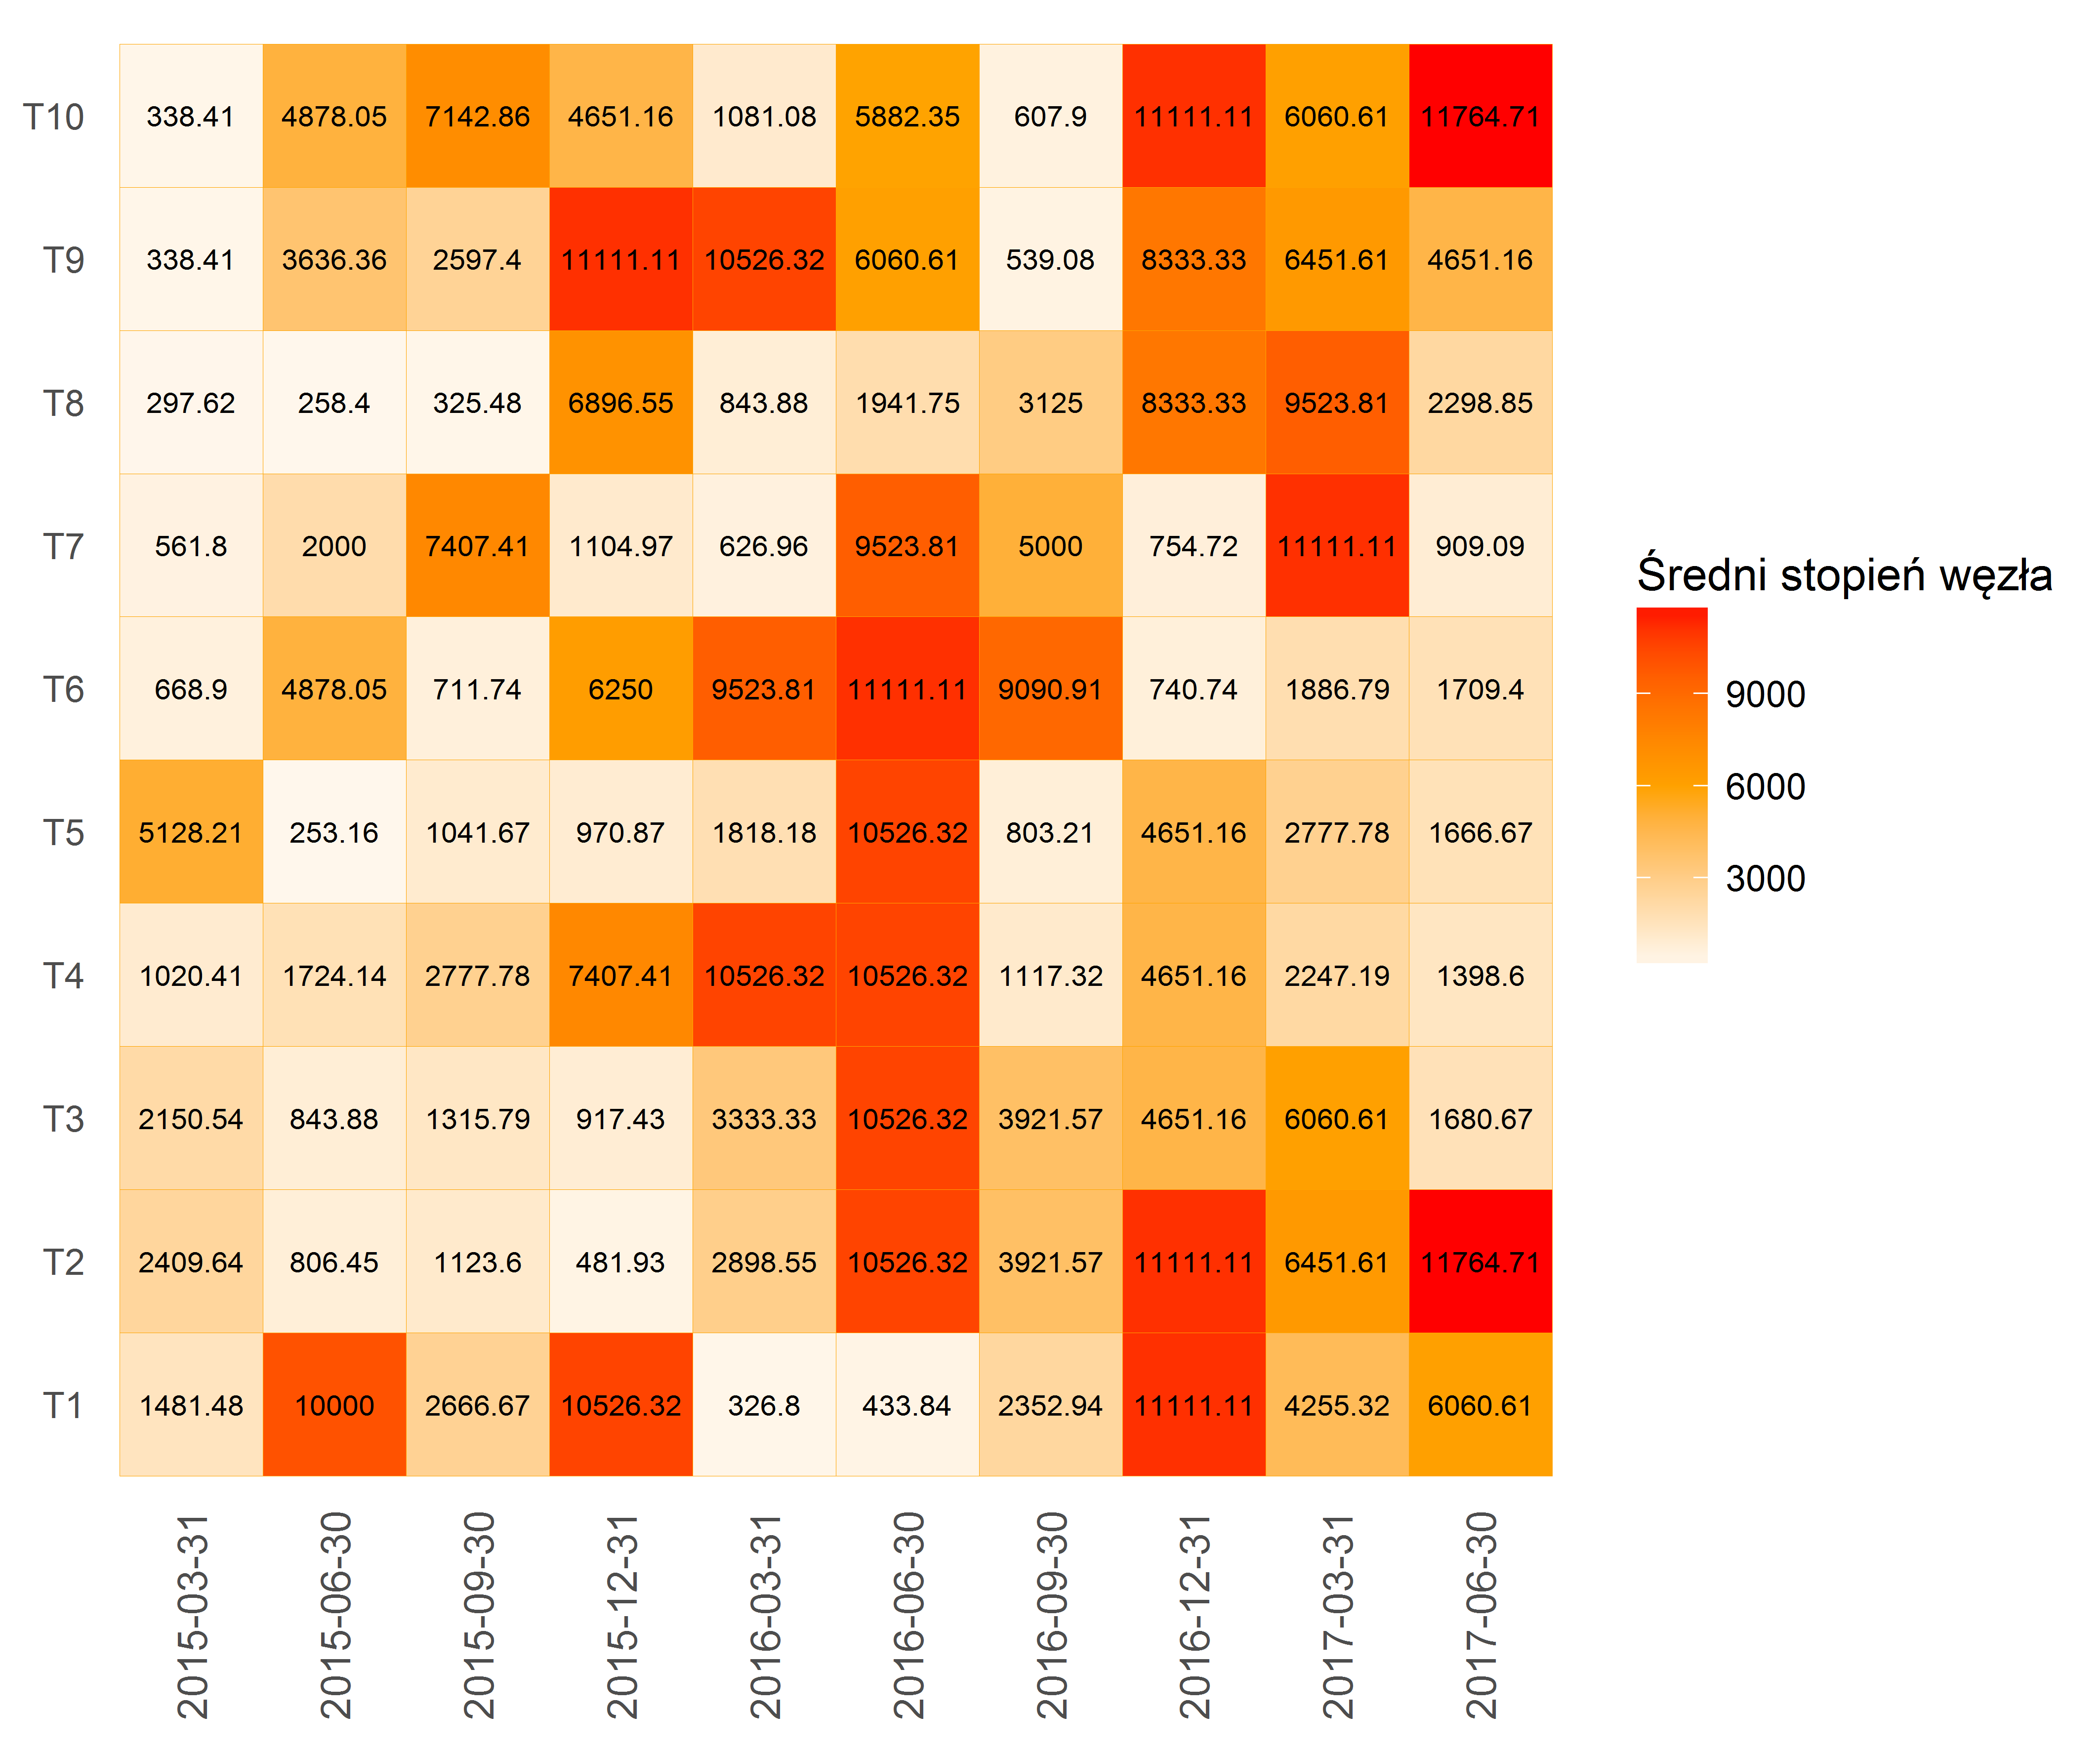
\includegraphics[width=\chartsWidth\linewidth]{pictures/sredni_stopien_wezla/sredni_stopien_wezla_hm.png}
   \caption{Mapa cieplna średniego stopnia węzła sieci dla 10 prób w 10 okresach.}
   \label{fig:sw1} 
\end{figure}
\begin{figure}[H]
   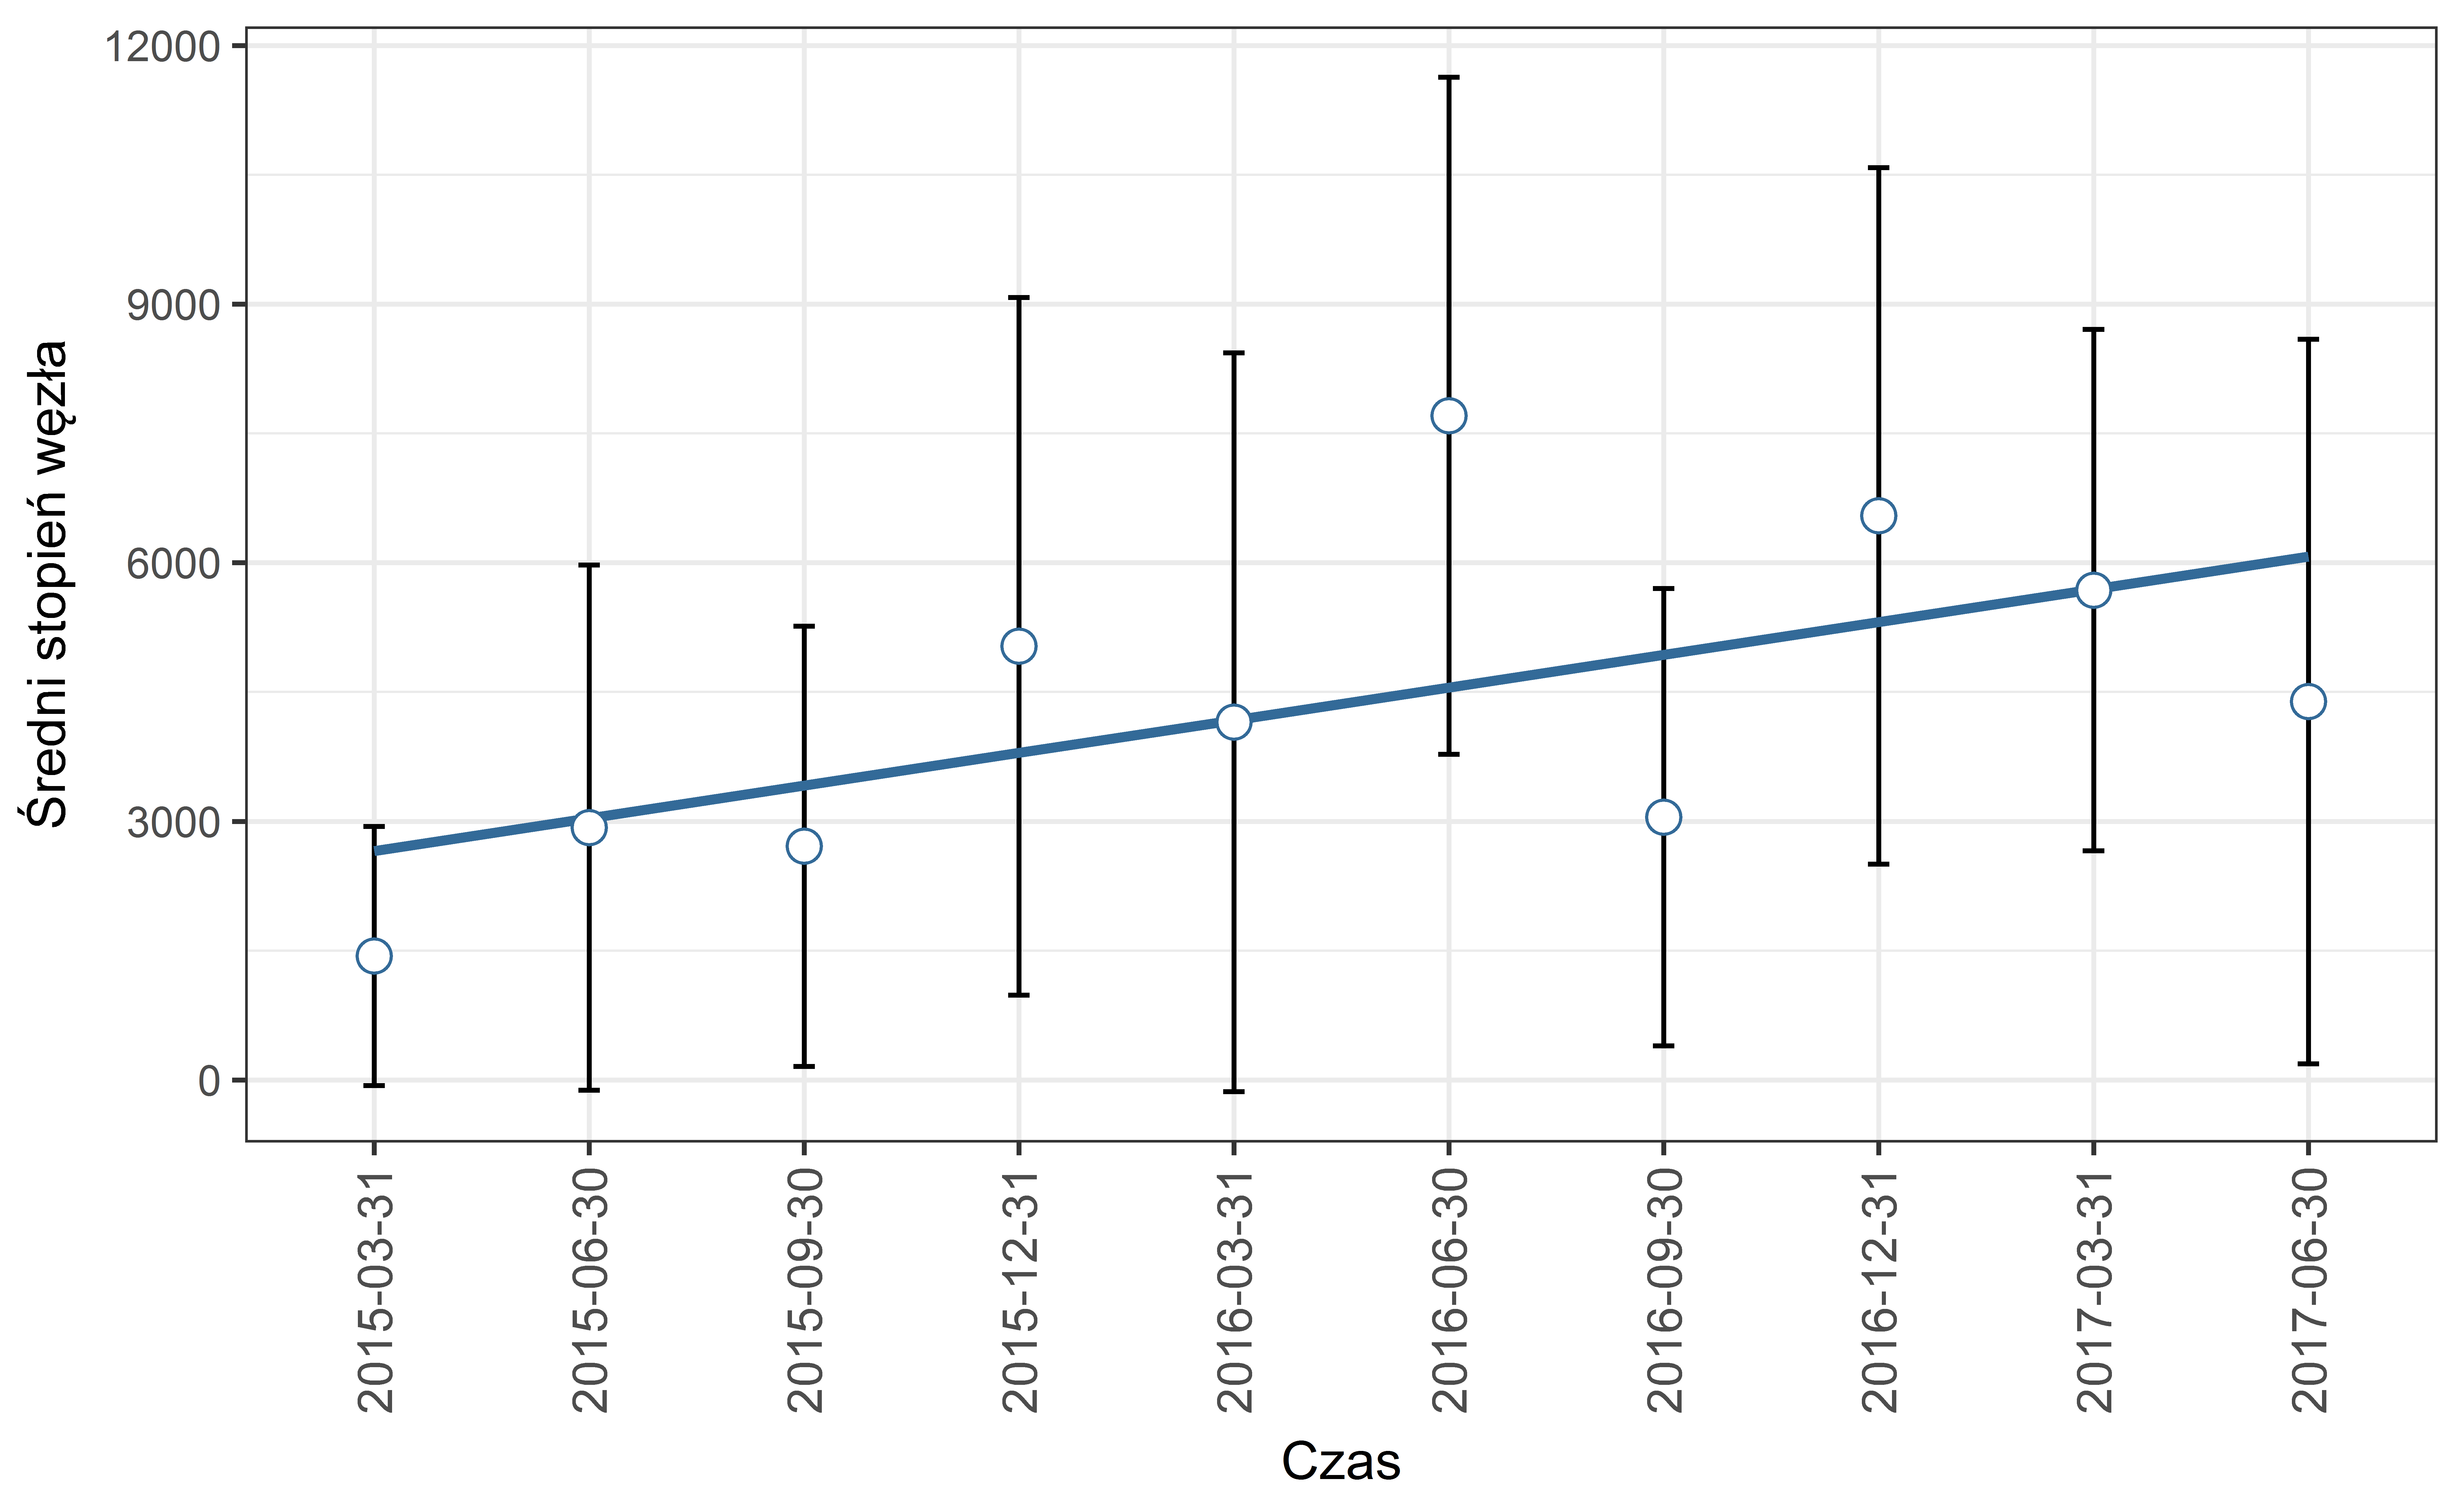
\includegraphics[width=\chartsWidth\linewidth]{pictures/sredni_stopien_wezla/sredni_stopien_wezla_sda.png}
   \caption{Regresja liniowa średniego stopnia węzła sieci dla 10 okresów z odchyleniem standardowym.}
   \label{fig:sw2}
\end{figure}
\newpage
\begin{figure}[H]
   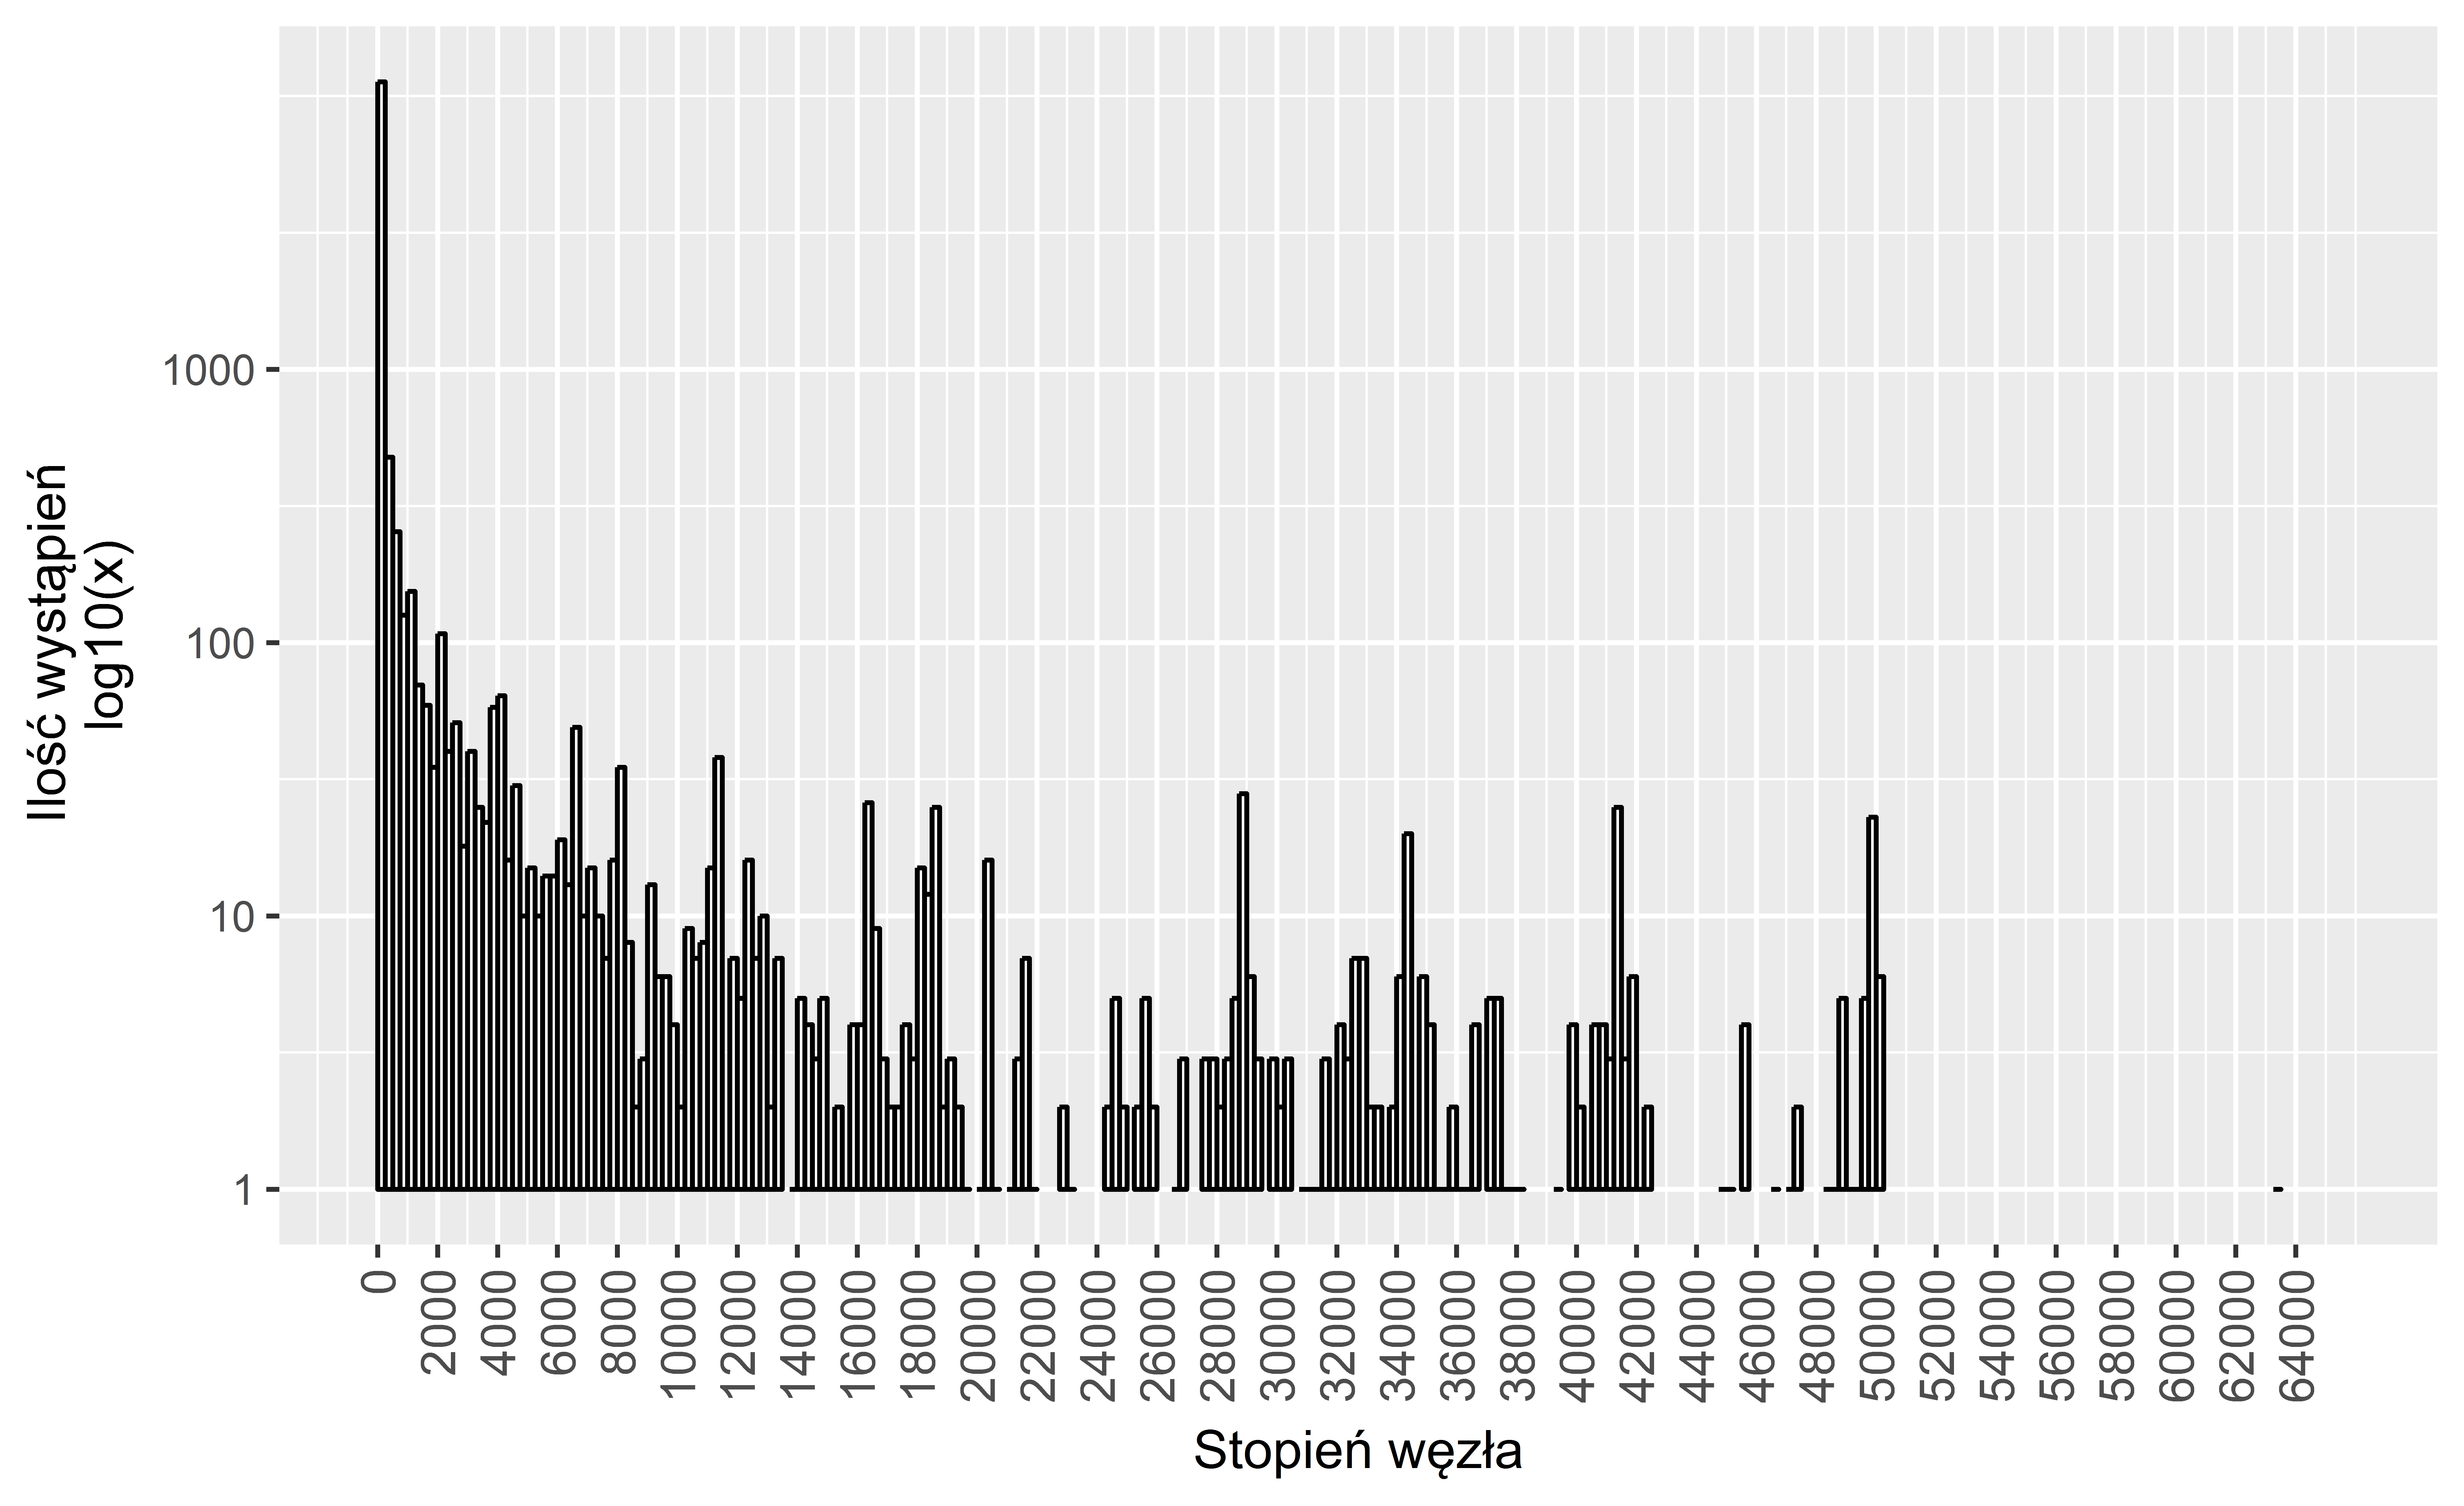
\includegraphics[width=\chartsWidth\linewidth]{pictures/sredni_stopien_wezla/sredni_stopien_wezla_hist.png}
   \caption{Histogram średniego stopnia węzła łączny dla wszystkich próbek.}
   \label{fig:sw3}
\end{figure}

\subsection{Badanie średniej centralności węzła}
\label{srednia_centralnosc}
\indent Centralność węzła $v$ jest miarą bazującą na własności grafu polegającej na znalezieniu \textit{najkrótszych ścieżek w~grafie}. Centralność węzła opiera się na znalezieniu wszystkich możliwych najkrótszych ścieżek w grafie pomiędzy połączonymi węzłami, które następnie grupowane są na ścieżki przechodzące przez węzeł $v$. Średnia centralność węzła dana jest wzorem 
\begin{equation}
\label{eq:centralnosc}
  \frac{\sum_i^n\sum_{s \ne v_i \ne t}^{}\frac{\sigma_{st}(v_i)}{\sigma_{st}}}{n}
\end{equation} 
gdzie $\sigma_{st}$ jest liczbą wszystkich najkrótszych ścieżek przechodzących od węzła~$s$ do węzła~$t$, $\sigma_{st}(v_i)$ jest liczbą wszystkich najkrótszych ścieżek przechodzących od węzła~$s$ do węzła~$t$ przez węzeł~$v_i$, a $n$ jest liczbą wszystkich węzłów w grafie\cite{barabasi2016network}.

\indent W badanej sieci centralność pojedynczej transakcji stanowi informację o jej znaczeniu dla całej sieci. Taka transakcja może zawierać adresy wejściowe jak i wyjściowe, które są mniej lub bardziej znaczące dla istnienia sieci, jednakże można stwierdzić, że im mniej adresów użytych w transakcji, a większa centralność transakcji, tym większe ich znaczenie. Zbudowana sieć bazuje na nieokreślonej wielkości zbiorach adresów w transakcji, więc pozwala zaobserwować ich znaczenie tylko jako jednostki. Duża centralność pojedynczej transakcji oznacza, że przekazywane przy jej pomocy środki są źródłem dla wielu innych transakcji. Średnia centralność wszystkich transakcji w próbce wyznacza zatem średnią istotność każdej transakcji w próbce.

\indent Na podstawie mapy cieplnej~\ref{fig:sc1} stworzonej dla omawianej właściwości sieci wywnioskowano, przy założeniu zignorowania granicznych wyników, że w badanych okresach średnia centralność transakcji w próbach jest zbliżona. Zaobserowano również, że dla większości badanych próbek w kolejnych okresach istotność transakcji w sieci spada. Potwierdza to wykres~\ref{fig:sc2}, który przedstawia trend spadkowy średniej centralności transakcji w sieci, ciągłe zagęszczanie sieci oraz wzrost ilości wykonywanych transakcji w czasie, co zostało już omówione w poprzednich analizach.

\indent Na histogramie~\ref{fig:sc3} prezentującym ilość wystąpień poszczególnych wartości centralności węzłów dla wszystkich próbek razem zaobserwowano zdecydowaną przewagę węzłów o małej centralności. Determinuje to zdecydowany spadek znaczenia pojedynczej transakcji w sieci.

\indent Dodatkowo zauważono widoczną zależność pomiędzy średnią centralnością węzłów, a~średnim stopniem węzła. Im mniejsza centralność węzłów tym większy stopień węzła, co oznacza, że sieć wciąż ewoluuje i zmienia swoją topologię w topologię siatki. 

\begin{figure}[H]
\centering
   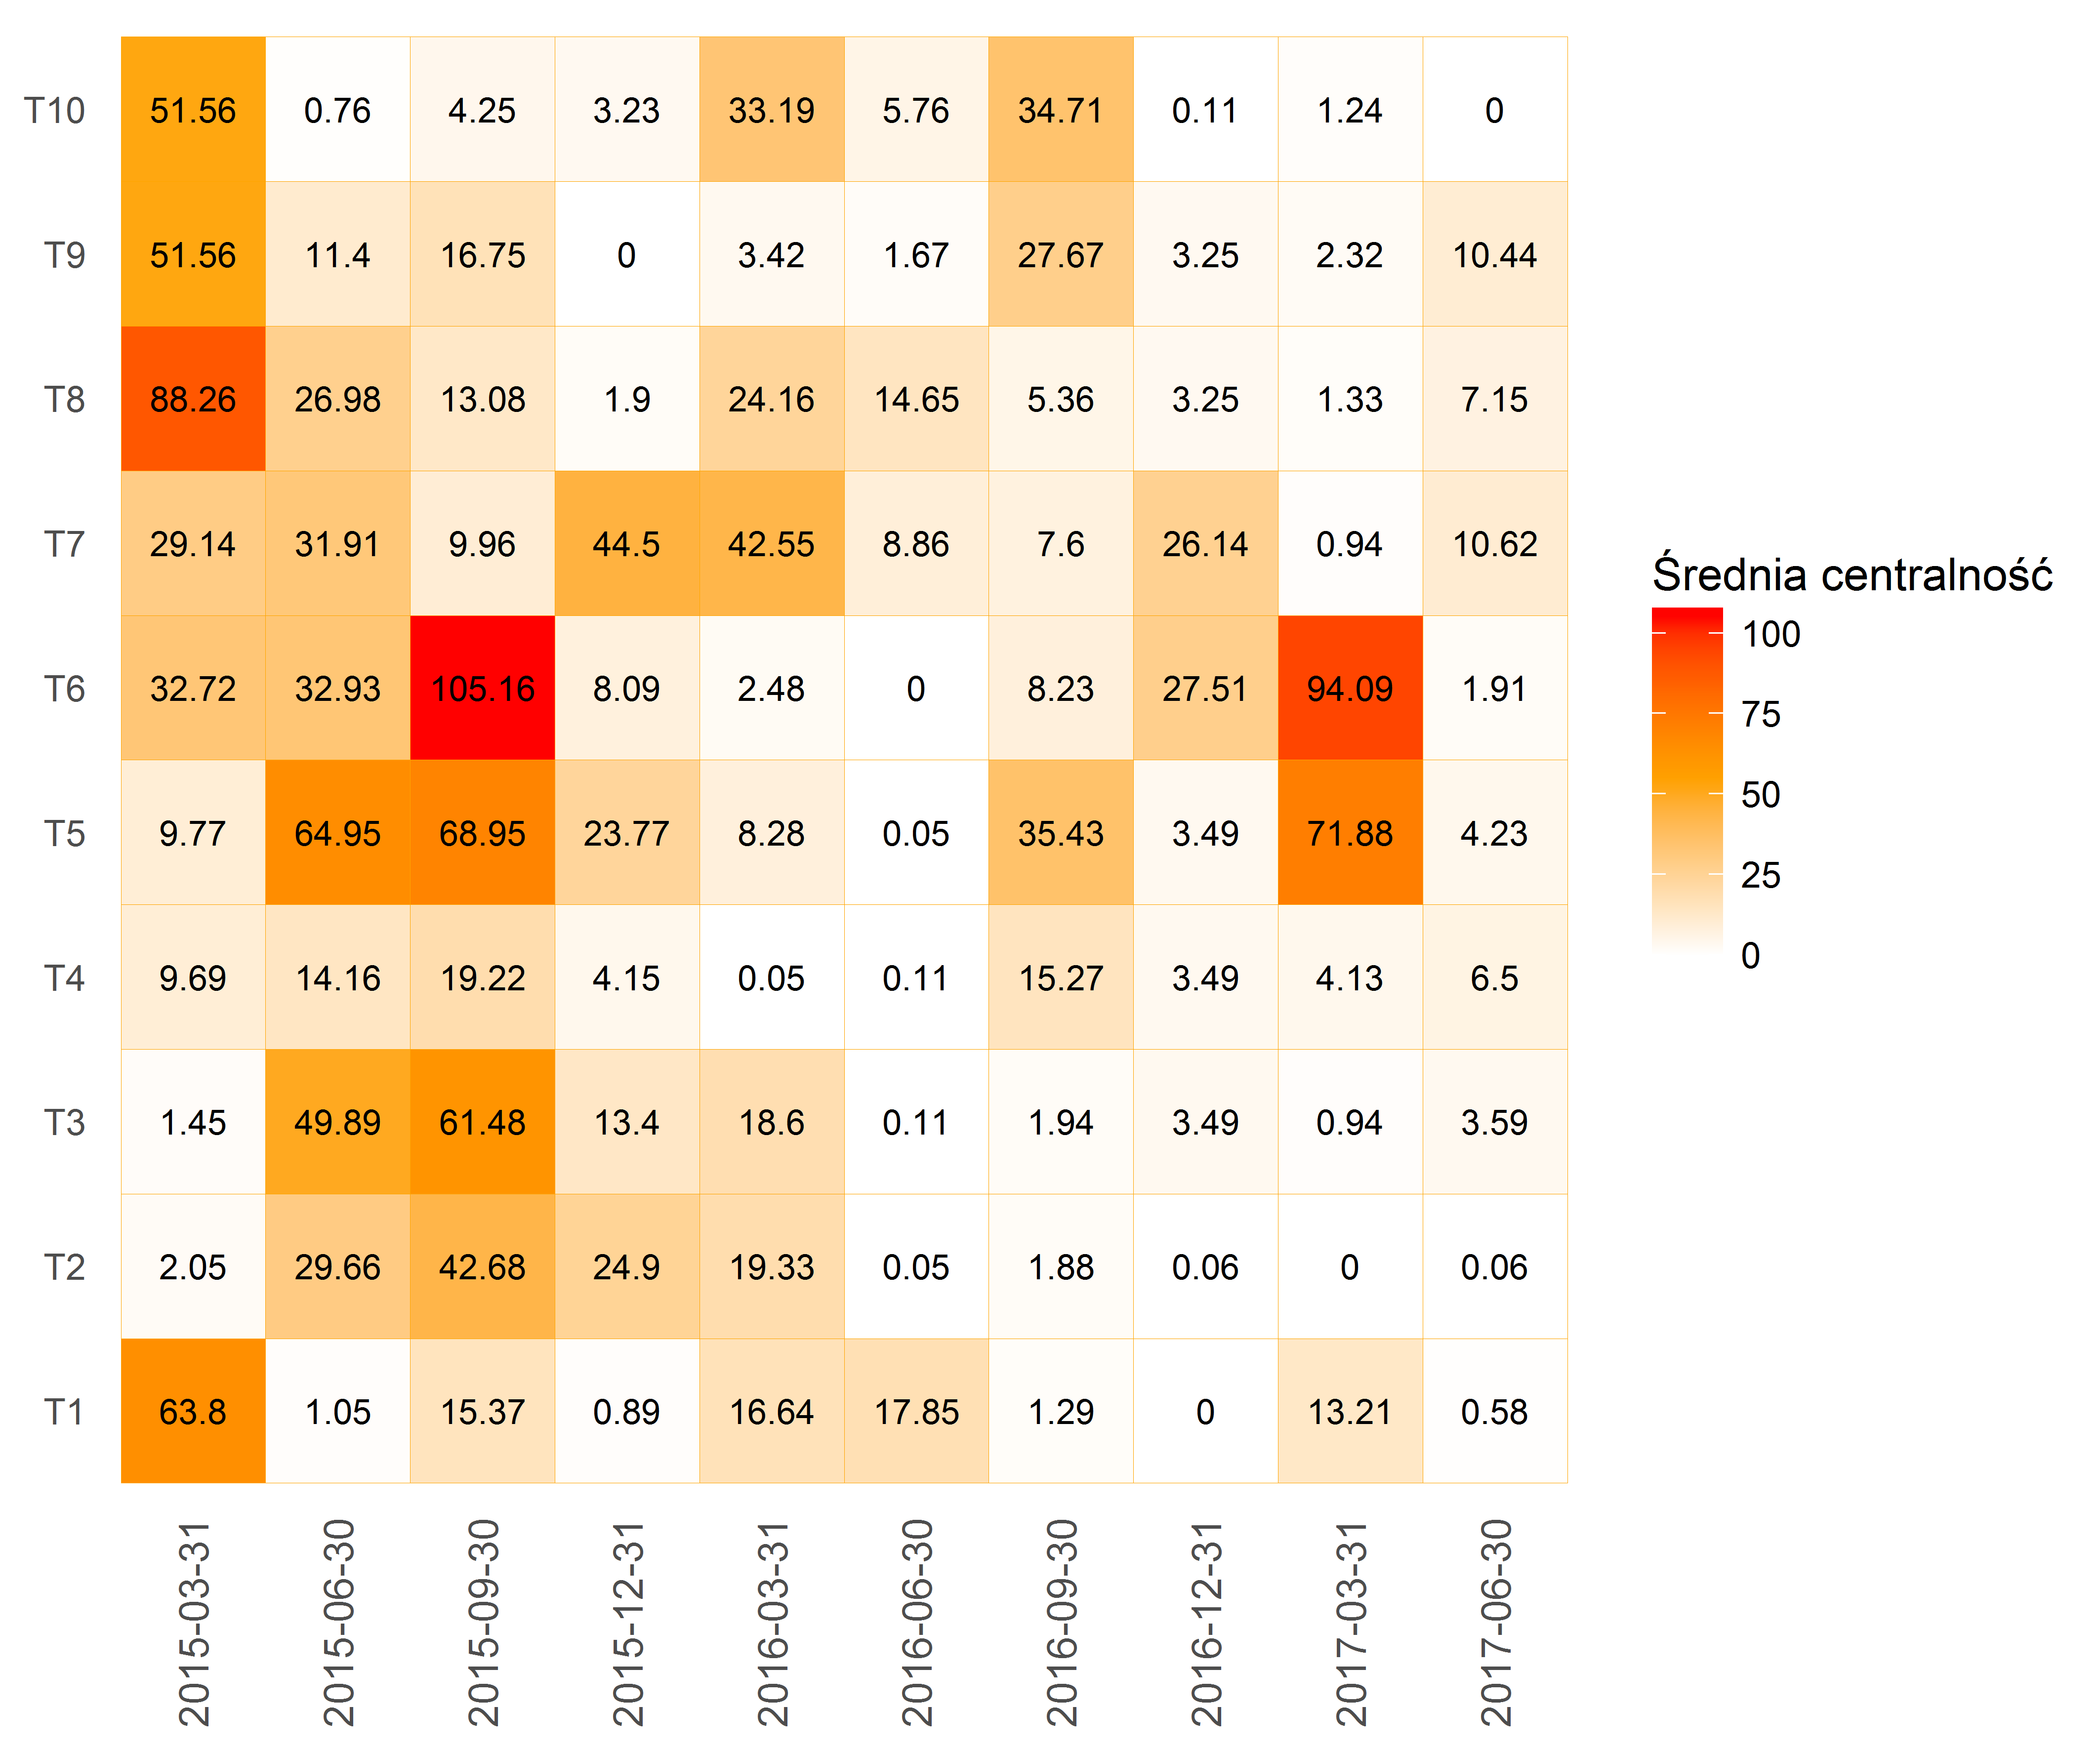
\includegraphics[width=\chartsWidth\linewidth]{pictures/srednia_centralnosc/srednia_centralnosc_hm.png}
   \caption{Mapa cieplna średniej centralności węzłów w sieci dla 10 prób w 10 okresach.}
   \label{fig:sc1} 
\end{figure}
\begin{figure}[H]
\centering
   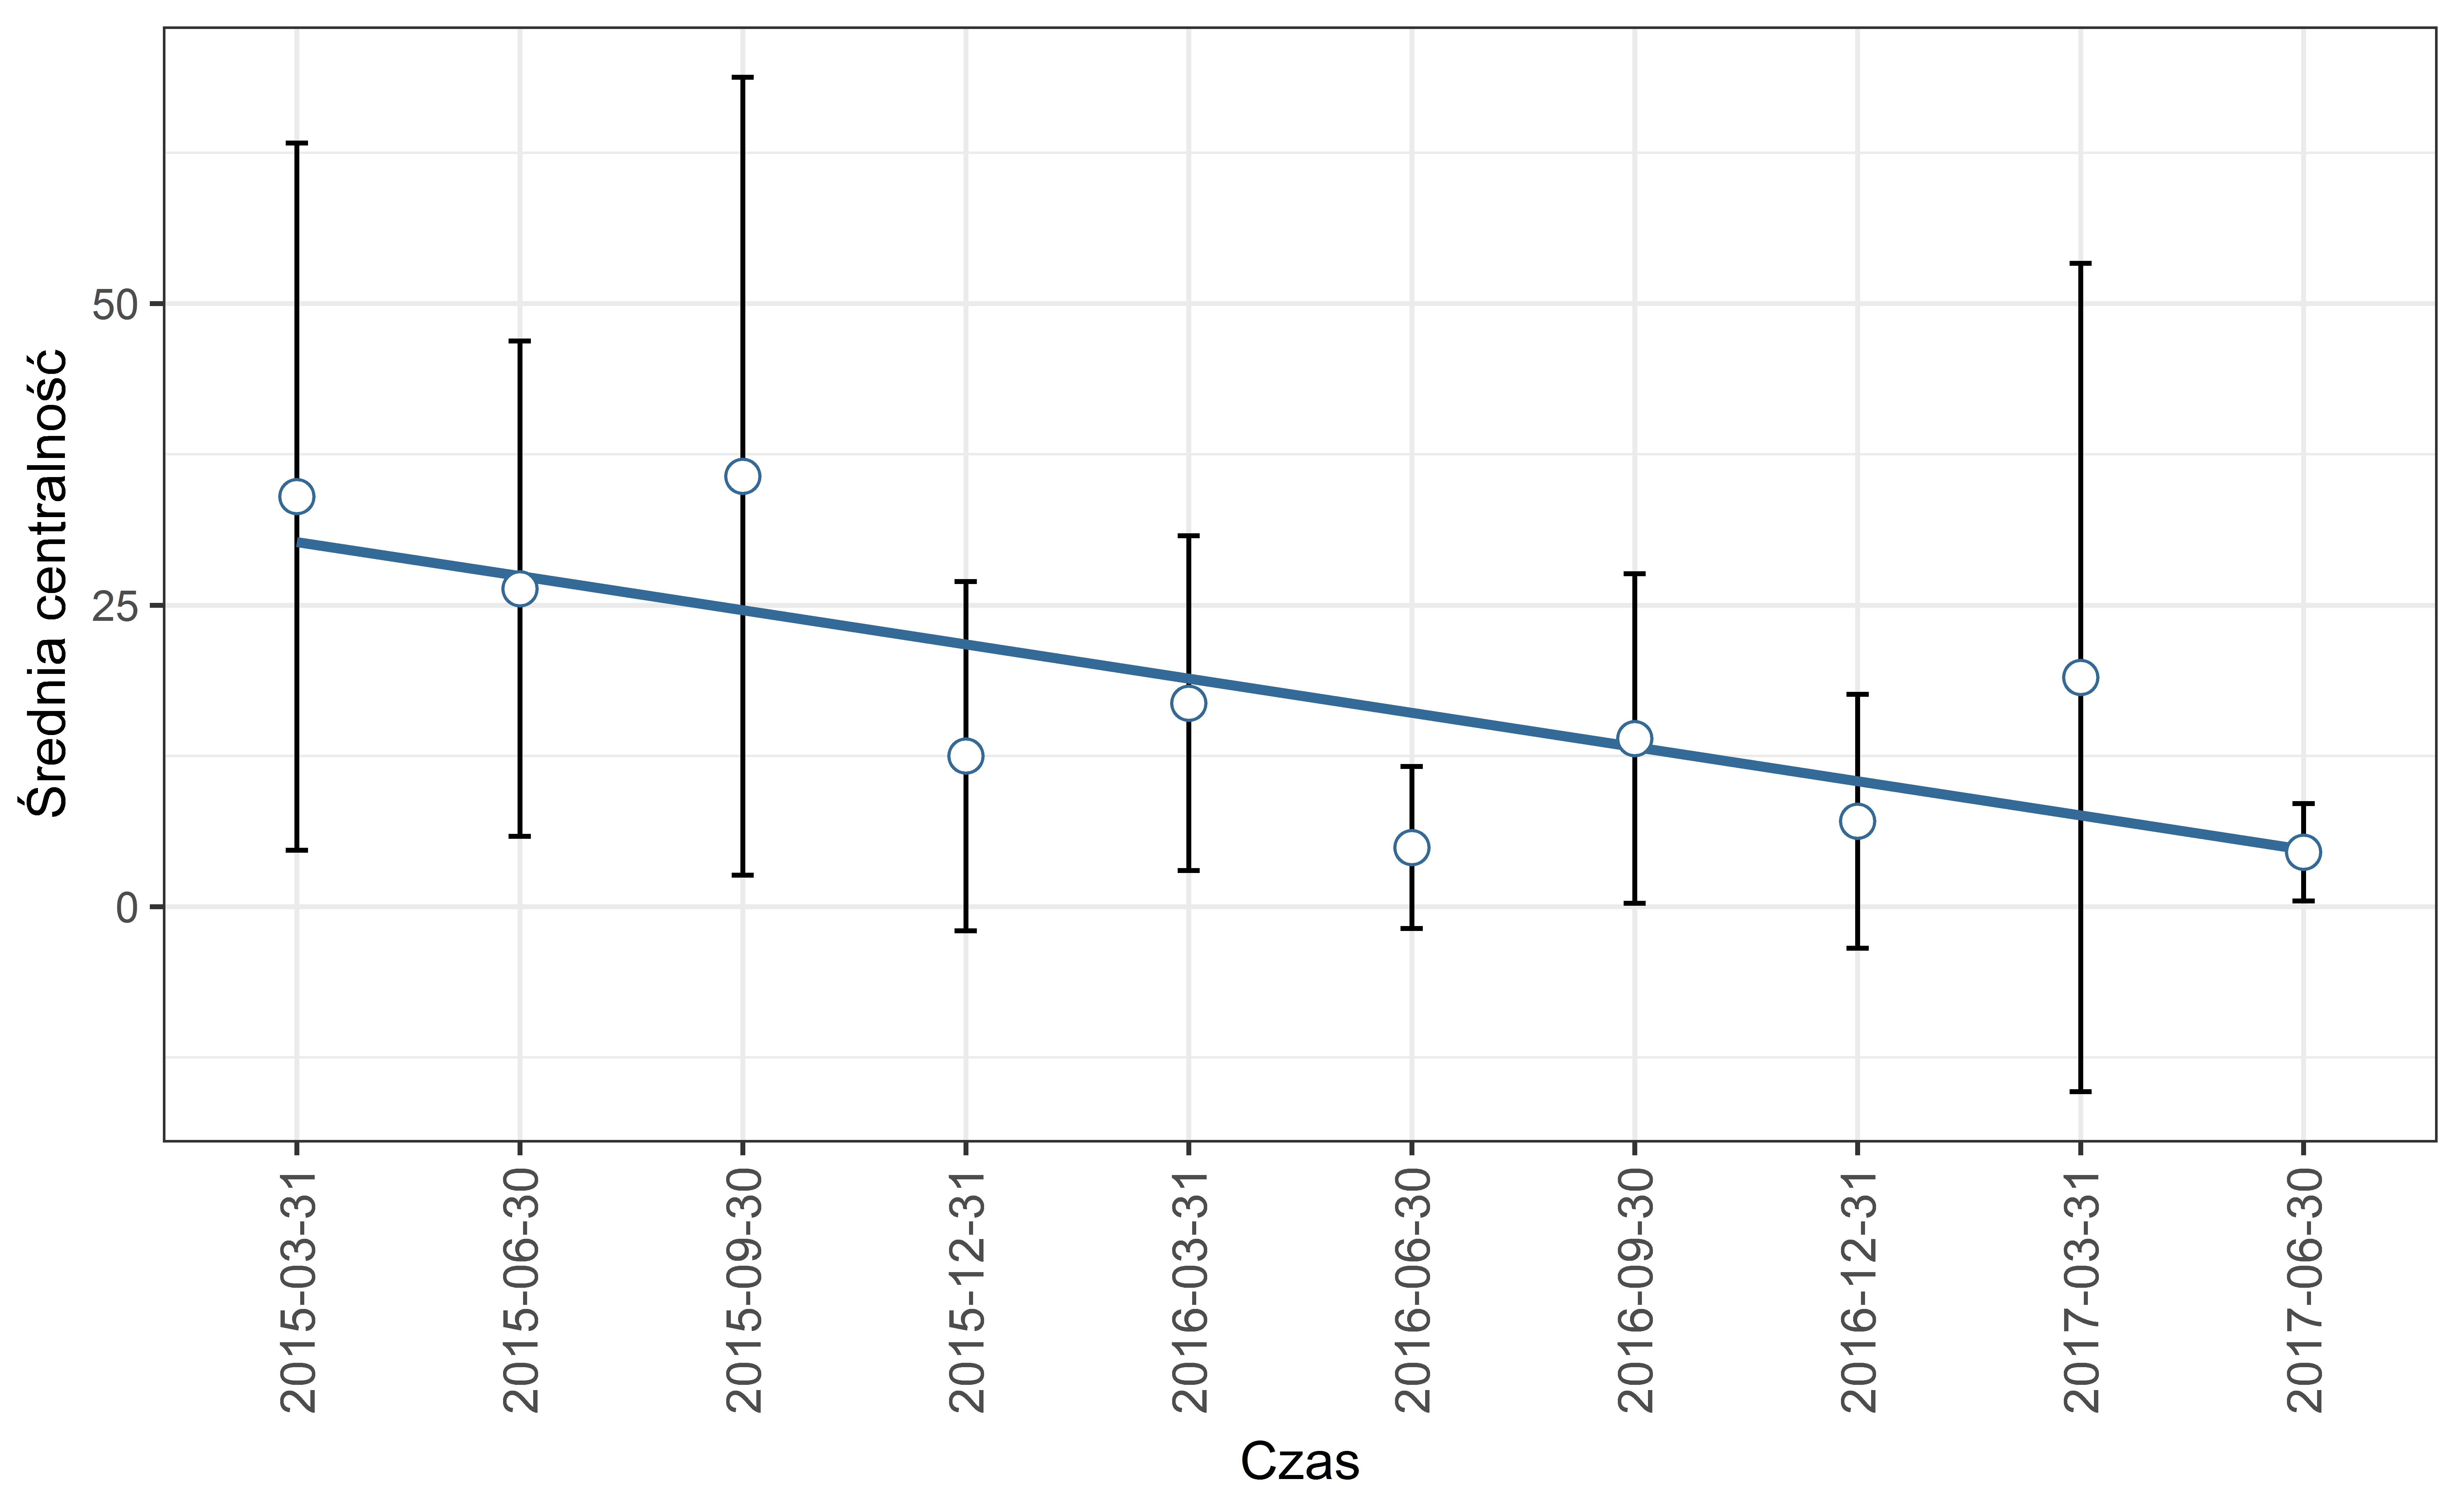
\includegraphics[width=\chartsWidth\linewidth]{pictures/srednia_centralnosc/srednia_centralnosc_sda.png}
   \caption{Regresja liniowa średniej centralności węzłów w sieci dla 10 okresów z~odchyleniem standardowym.}
   \label{fig:sc2}
\end{figure}
\begin{figure}[H]
\centering
   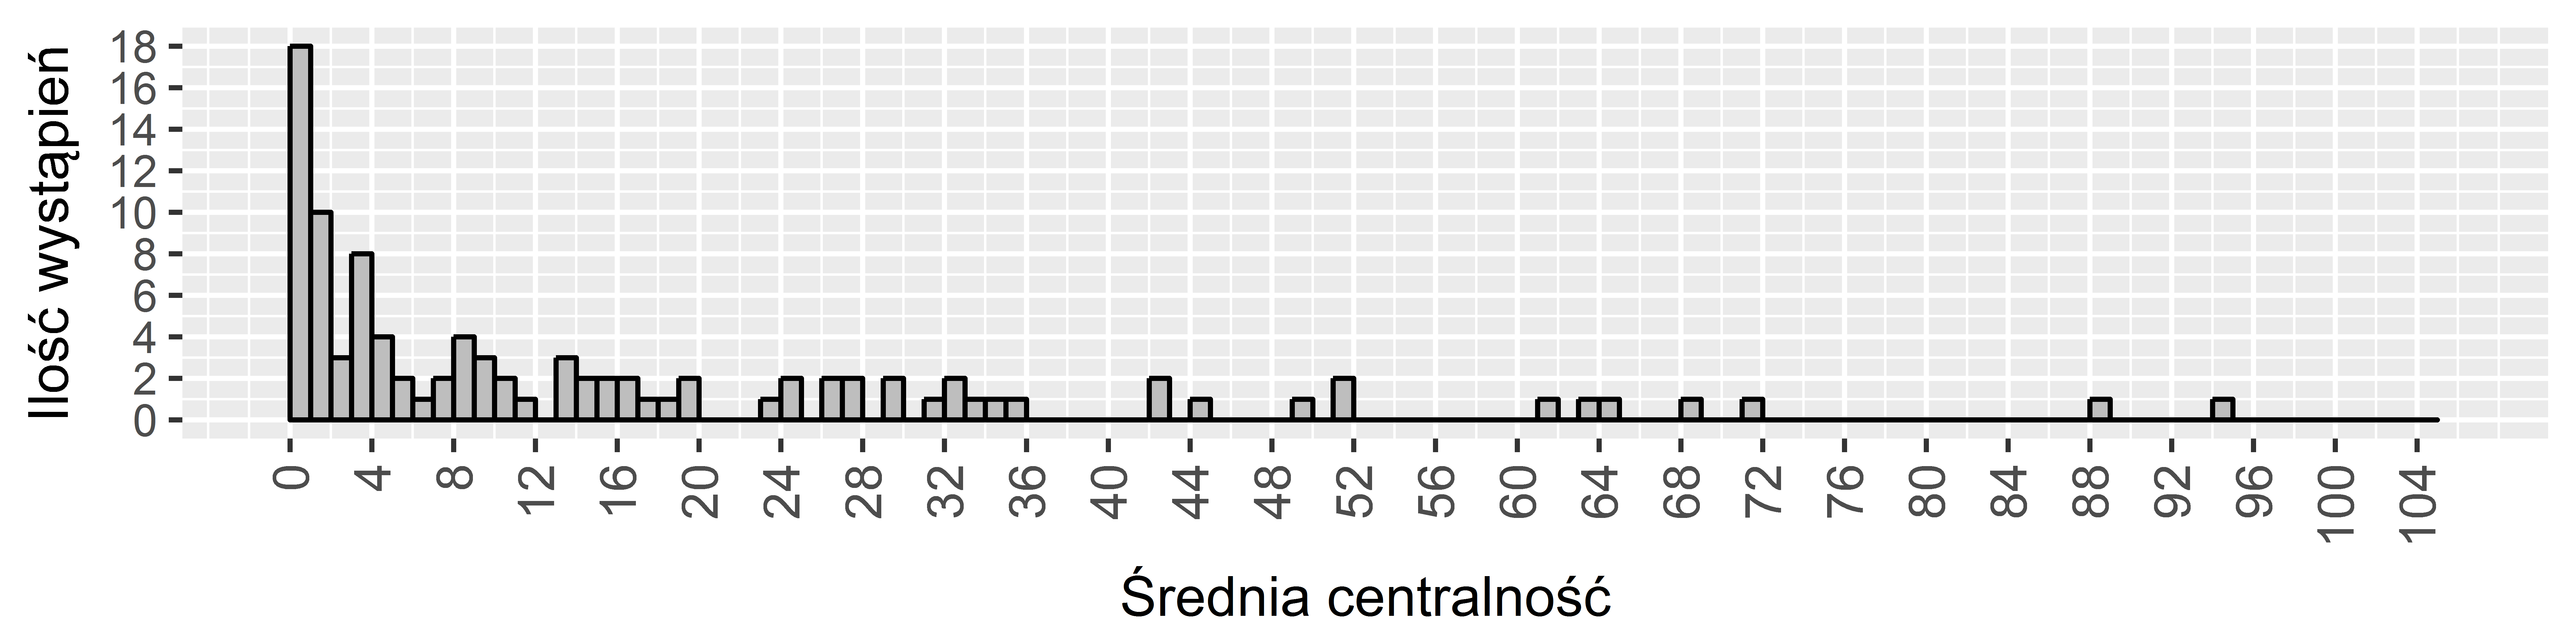
\includegraphics[width=\chartsWidth\linewidth]{pictures/srednia_centralnosc/srednia_centralnosc_hist.png}
   \caption{Histogram centralności węzłów w sieci łączny dla wszystkich prób.}
   \label{fig:sc3}
\end{figure}

\subsection{Badanie średniej wartości transakcji}
\label{wartosc_transakcji}
\indent Średnią wartości transakcji jest miarą bezpośrednio związaną z typem badanej sieci. Oznacza średnią wartości bitcoinów, która wiąże ze sobą węzły reprezentujące transakcje, tworząc graf ważony. Wartość bitcoinów pomiędzy dwoma węzłami stanowią wagę krawędzi przejścia pomiędzy nimi. Średnia wartość transakcji można zapisać jako
\begin{equation}
\label{eq:wartosc_transakcji}
\frac{\sum_{i}^{n} \omega(e_i)}{n}
\end{equation}
gdzie $\omega(e_i)$ oznacza wagę przejścia (ilość bitcoinów) przez krawędź łączącą dwa węzły (transakcje), a~$n$~oznacza ilość wszystkich krawędzi (połączeń pomiędzy transakcjami). 

\indent Przeprowadzone badanie wykazało, że w różnych okresach wartość mierzona pojedynczych próbek znacząco odbiega od pozostałych, co może wpływać na ogólny wynik badań.
Na mapie cieplnej~\ref{fig:wt1} przedstawiono rezultat tych badania. Możliwe jest, że odbiegające próbki stanowią przekazy środków pomiędzy adresami giełd lub giełdą, a~innymi uczestnikami sieci. Wskazują na to znacząco wyższe sumy łączące transakcje. Chwilowe pominiecie tych wyników pozwala na stwierdzenie, że ilości przekazywanych środków we wszystkich okresach są bardzo porównywalne. Niedużą tendencję wzrostową można zauważyć w ostatnich trzech okresach, co potwierdza wykres~\ref{fig:wt2} przedstawiający rosnący trend średniej wartości transakcji. 

\indent Transakcje do badań wybierane było kolejno z bloków, a priorytety kolejno podpisywanych transakcji zależą między innymi od wniesionej opłaty przez zleceniodawców. Przy szybkim wzroście wartości bitcoina oraz założeniu, że giełdy lub uczestnicy sieci prowadzący duże wymiany wnoszą większe opłaty (w celu zapewnia jak najszybszego przekazu środków) można również zauważyć wzrost zainteresowania, w stosunku do okresów poprzednich, bogatych instytucji prowadzących interesy w sieci Bitcoin. Niestety z~powodu dużej anonimowości uczestników sieci wyciągnięty wniosek nie jest niepodważalny. 
\newpage
\indent Przykładem na aktywności giełd w badanych próbach może być transakcja\\\texttt{b0acc2caa54197dd10aa02bef7df8b54a304716f5e0801dca2dd3a9c26f130d8} z bloku\\ \texttt{00000000000000000229200fbabedffc445a4911d1d6603d2962d564c1678f5c} z próby \textit{T8}, przy pomocy której przekazano \texttt{541.79706464} bitcoinów. Wśród adresów wyjściowych jak i adresów wejściowych tej transakcji odnaleziono adresy jednej z dużych giełd \textit{Poloniex.com}\cite{poloniex}:
\begin{itemize}
\item[--] \texttt{12cgpFdJViXbwHbhrA3TuW1EGnL25Zqc3P}
\item[--] \texttt{17A16QmavnUfCW11DAApiJxp7ARnxN5pGX}
\end{itemize}
Obecność transakcji zlecanych przez giełdy zwiększają średnią wartość transakcji w próbach, dlatego też próby, których średnia wartość transakcji znacząco odbiega od reszty może wskazywać na ich aktywność.

\begin{figure}[H]
\centering
   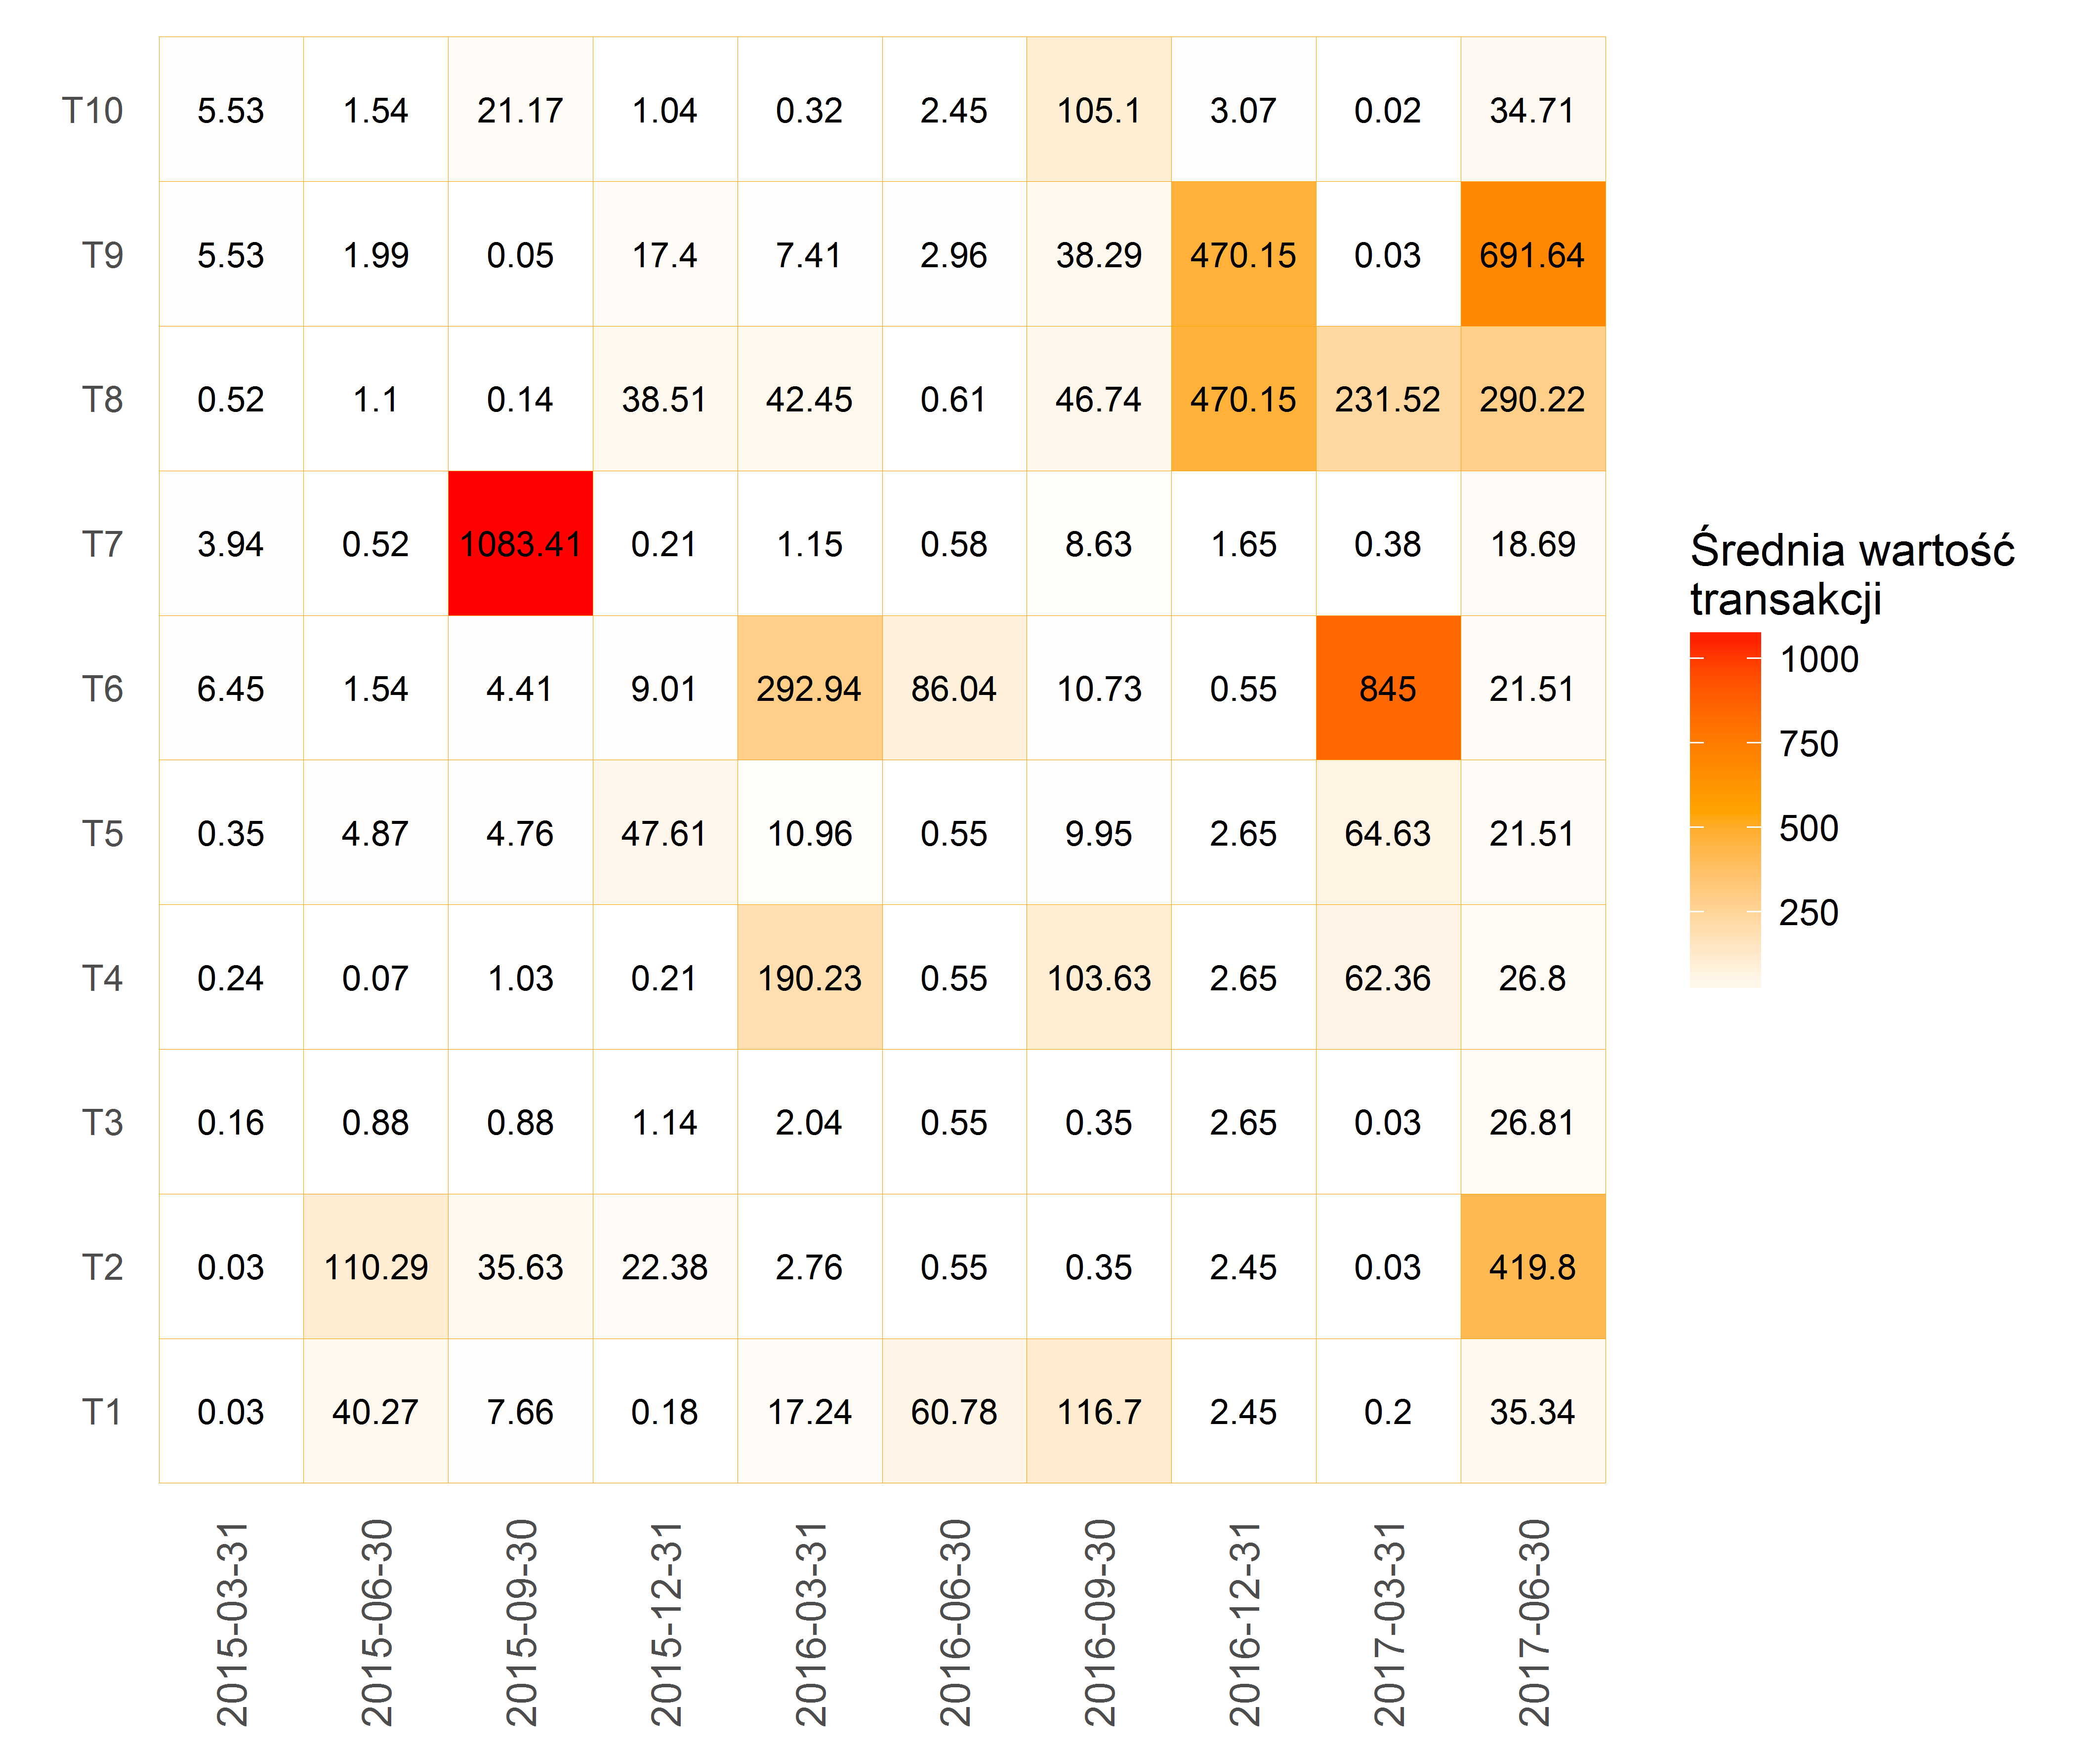
\includegraphics[width=\chartsWidth\linewidth]{pictures/wartosc_transakcji/wartosc_transakcji_hm.png}
   \caption{Mapa cieplna średniej wartości transakcji w sieci dla 10 prób w 10 okresach.}
   \label{fig:wt1} 
\end{figure}
\newpage
\begin{figure}[H]
\centering
   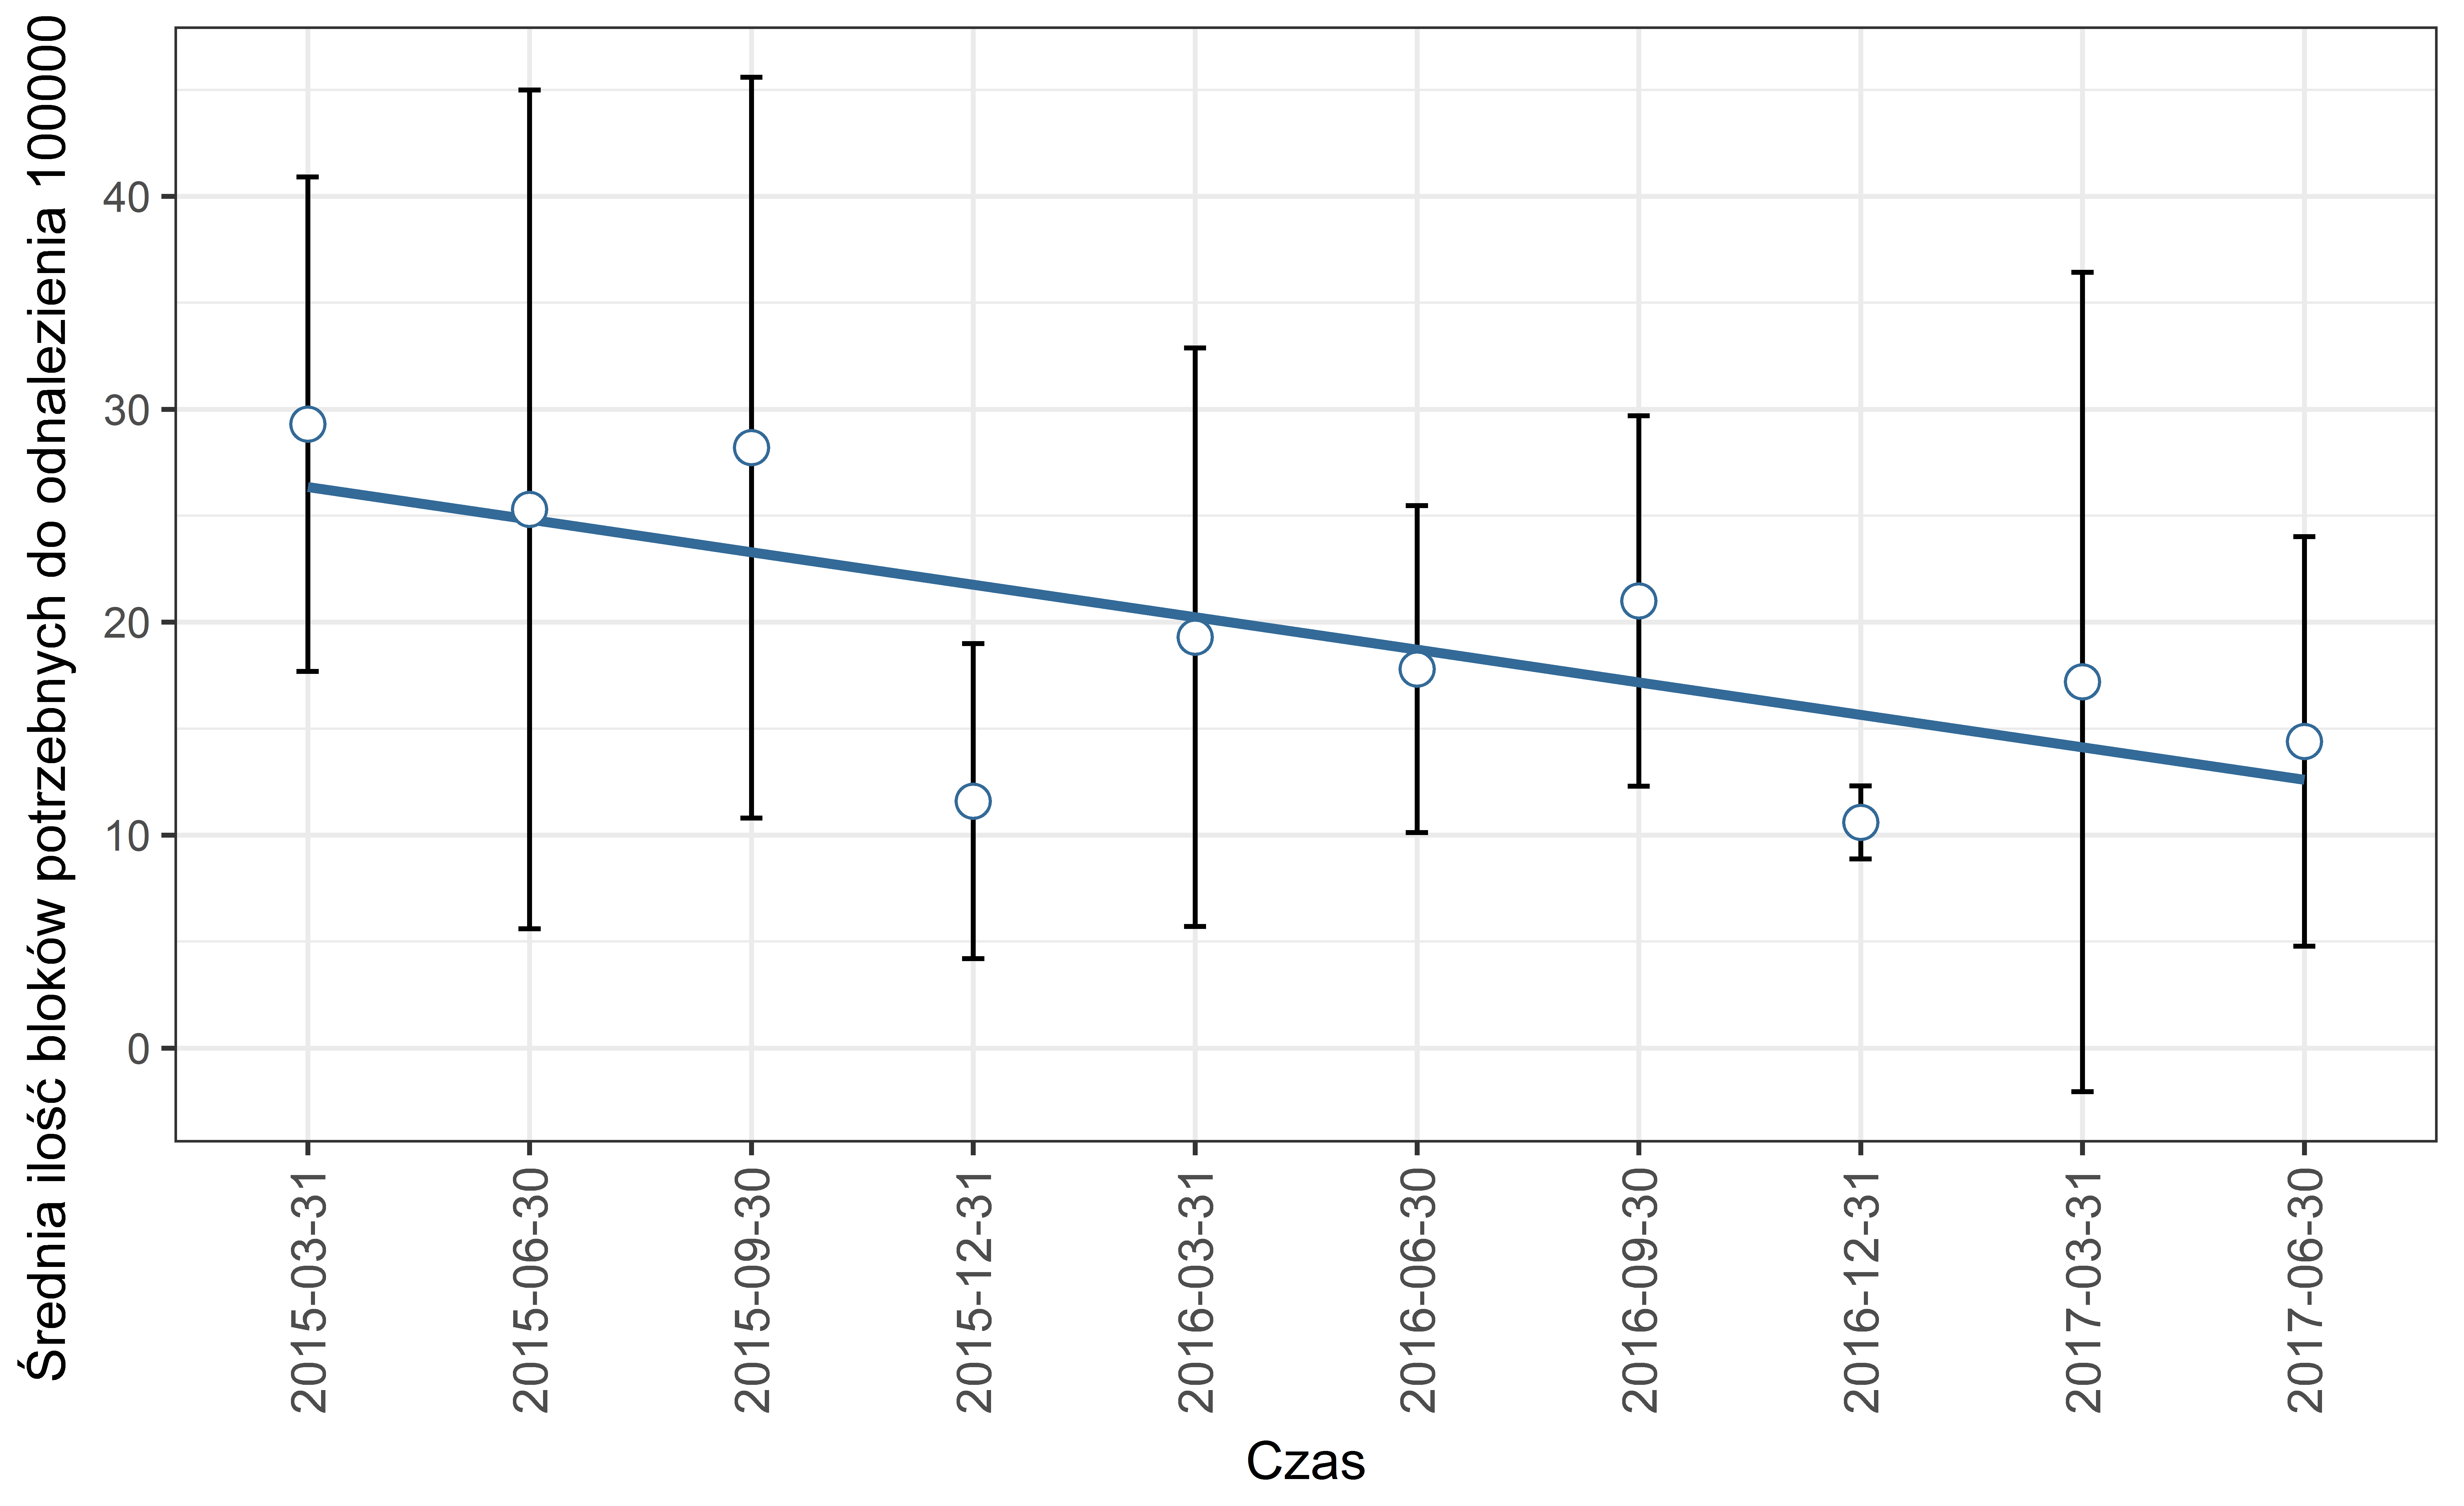
\includegraphics[width=\chartsWidth\linewidth]{pictures/wartosc_transakcji/wartosc_transakcji_sda.png}
   \caption{Regresja liniowa średniej wartości transakcji w sieci dla 10 okresów z~odchyleniem standardowym.}
   \label{fig:wt2}
\end{figure}


\subsection{Badanie ilości bloków}
\label{ilosc_blokow}
\indent Ilość bloków jest kolejną miarą związaną z rodzajem badanej sieci. Polega na zliczeniu wszystkich bloków, w których znajdują się transakcje dołączone do próbki sieci. Każda transakcja może być zawarta jedynie w jednym bloku, natomiast jeden blok może zawierać wiele transakcji, które zostały połączone w procesie budowania sieci. Informacje o przynależności węzłów (transakcji) do poszczególnych bloku zostały wyekstrahowane podczas budowania próbek sieci i stanowią w niniejszym badaniu metadane węzła. 

\indent Zliczenie ilość bloków, w których znajdują się wszystkie powiązane ze sobą węzły zostało zrealizowane poprzez znalezienie wszystkich unikalnych adresów bloków z transakcji.

\indent Na mapie cieplnej~\ref{fig:ib1} zaprezentowano ilość bloków potrzebną na znalezienie stu tysięcy połączeń pomiędzy transakcjami. Na podstawie przebadanych prób zaobserwowano zróżnicowanie badanej wartości w okresach. Duża ilość bloków oznacza małą aktywność uczestników sieci rozciągniętą w czasie, natomiast mała ilość bloków oznacza dużą aktywność uczestników sieci w określonych momentach czasu. Należy zauważyć, że prezentowana ilość bloków nie oznacza, że bloki te generowane były kolejno po sobie. Aktywność uczestników, zlecających transakcje, pozwalająca na budowę poszczególnych prób sieci mogła być nagła w~różnych momentach czasu. Zakładając jednak sytuację, w~której bloki budujące każdą z~prób występowały kolejno po sobie, a ilość bloków generowana w~sieci dziennie waha się w okolicy 170 bloków, stwierdzić można, że sieć składającą się ze stu tysięcy połączeń, która zaczyna się od pojedynczej transakcji, można zbudować w~nie dłużej niż w~przeciągu pół dnia. Prezentuje to ogrom badanej sieci, a zaprezentowany na wykresie~\ref{fig:ib2} trend spadkowy wskazuje na coraz szybszy jej rozwój. 

\begin{figure}[H]
\centering
   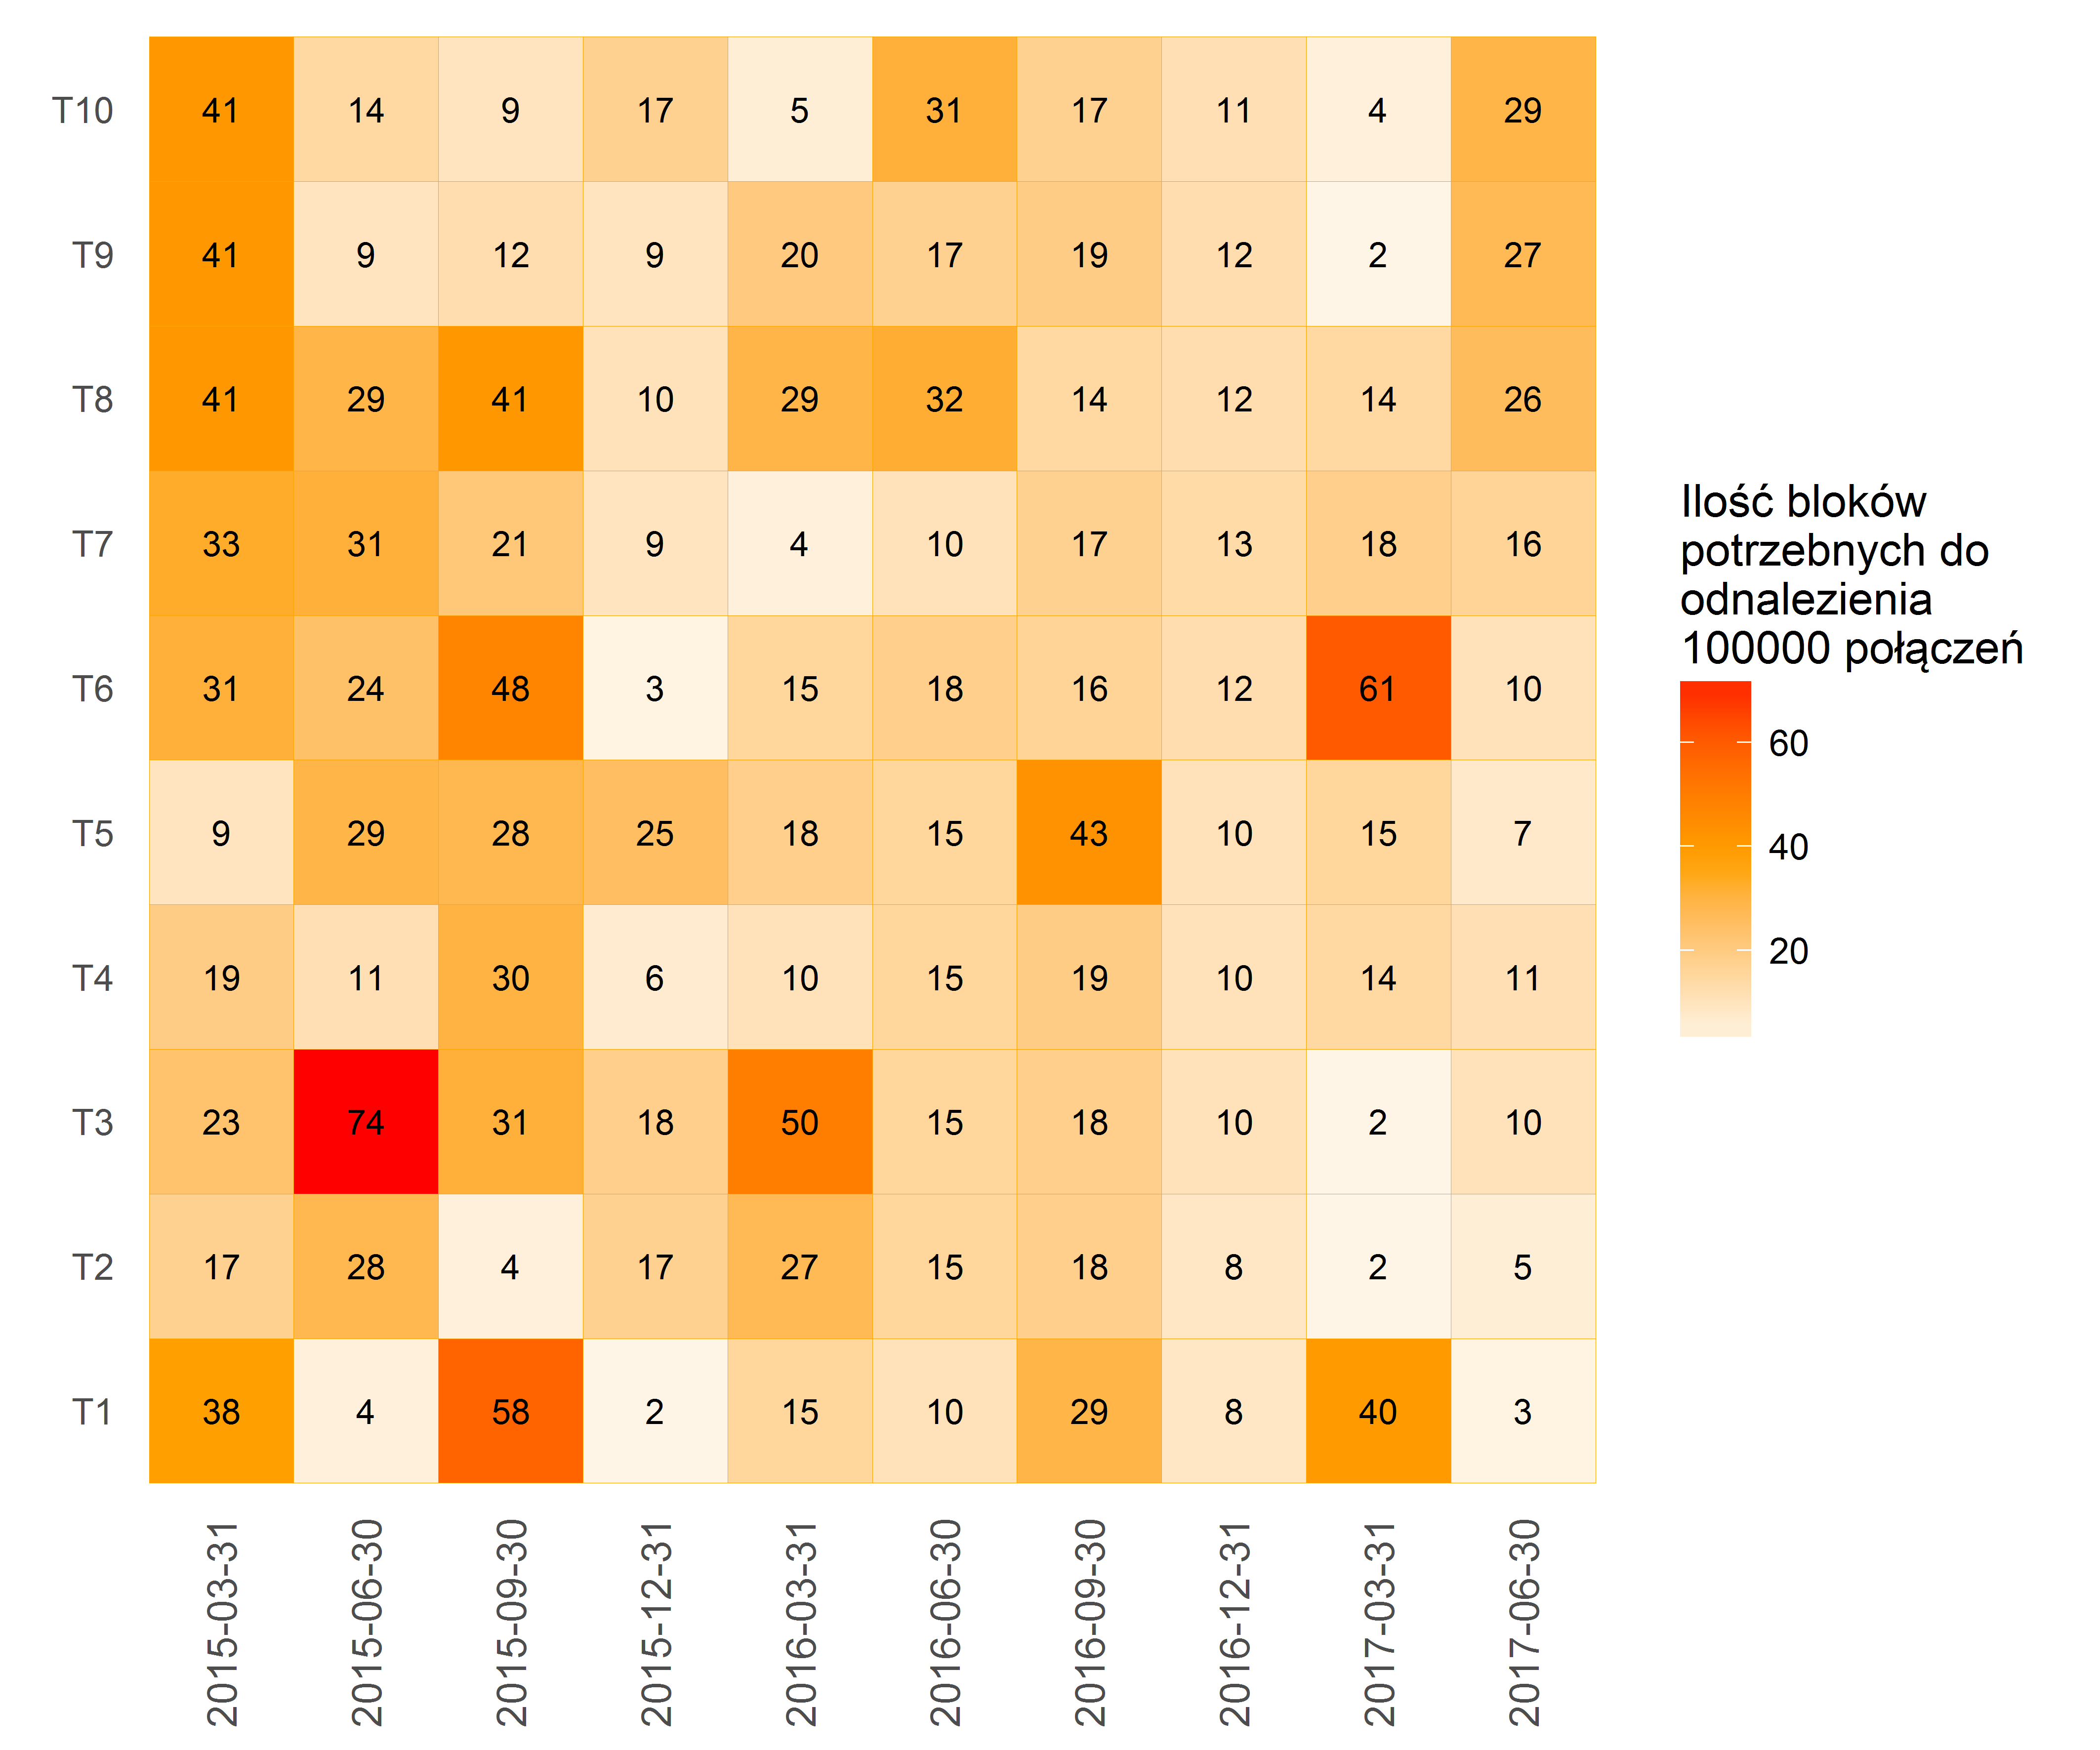
\includegraphics[width=\chartsWidth\linewidth]{pictures/ilosc_blokow/ilosc_blokow_hm.png}
   \caption{Mapa cieplna ilości bloków sieci potrzebnych na znalezienie 100000 połączeń dla 10 prób w 10 okresach.}
   \label{fig:ib1} 
\end{figure}
\begin{figure}[H]
\centering
   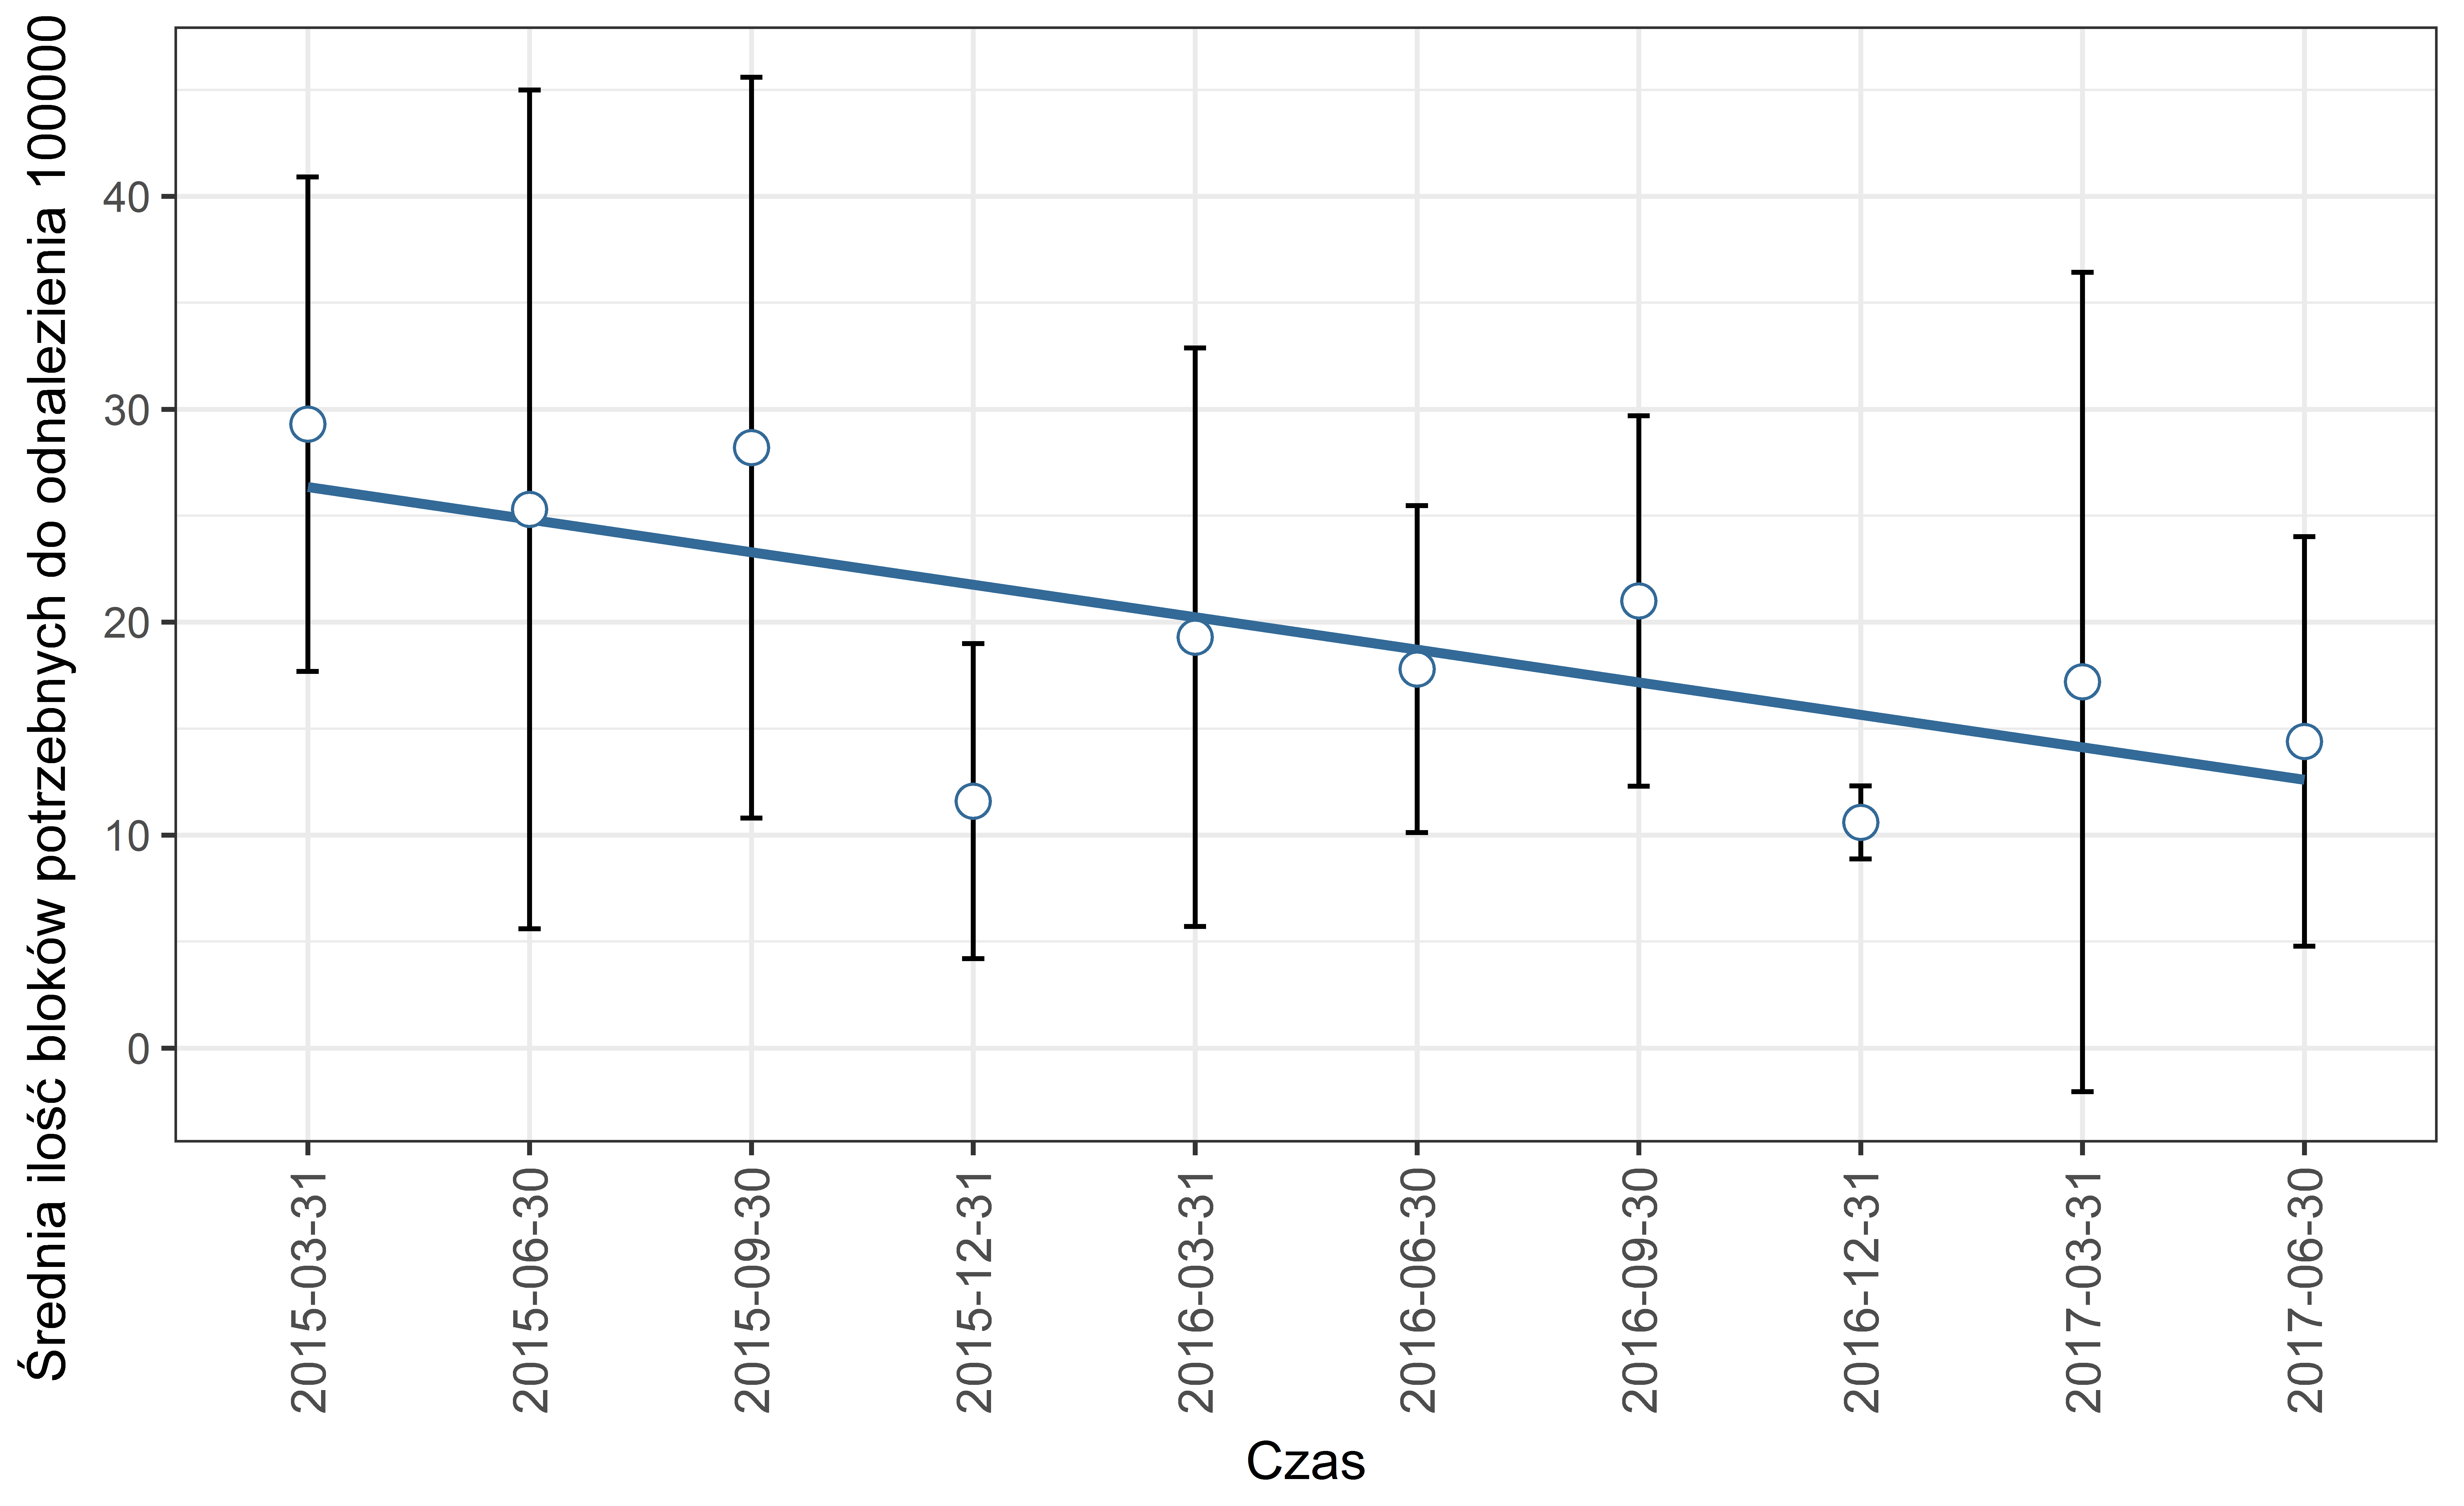
\includegraphics[width=\chartsWidth\linewidth]{pictures/ilosc_blokow/ilosc_blokow_sda.png}
   \caption{Regresja liniowa ilości bloków sieci potrzebnych na znalezienie 100000 połączeń dla 10 okresów z odchyleniem standardowym.}
   \label{fig:ib2}
\end{figure}

\newpage
\subsection{Badanie średniej różnicy czasów kolejnych transakcji}
\label{roznice_czasow}
\indent Badanie różnicy czasów kolejnych transakcji, to własność badanej sieci ściśle związana z~jej fachową stroną. Polega na zliczeniu różnic czasów realizowania kolejnych transakcji wstecz. Oparta jest na przeglądzie wszystkich możliwych ścieżek w sieci z~jednoczesnym ekstrahowaniem czasu $t(v_i)$ ich wykonania. W~konsekwencji pozwala to na wyliczenie różnic czasu pomiędzy transakcjami $v_i$ i $v_{i-1}$ w~ścieżkach. Średnia wartość różnic wykonywania kolejnych transakcji w~ścieżce jest ilorazem sumy wszystkich różnic w ścieżce i~ich ilości, co można zapisać jako
\begin{equation}
\label{eq:rckt1}
M(\sigma) = \frac{\sum_{i=1}^{n-1} t(\sigma(v_{i+1})) - t(\sigma(v_{i}))}{n-1}
\end{equation}
gdzie $M$ to średnia wartość różnic czasu kolejnych transakcji w~ścieżce $\sigma$, $t(\sigma(v_i))$ to czas wykonania i-tej transakcji w~ścieżce $\sigma$, $t(\sigma(v_{i+1}))$ to czas $t$ wykonania transakcji $v_{i+1}$ w~ścieżce $\sigma$, a $n$~to ilość połączeń pomiędzy transakcjami w ścieżce. 
\\ Średnią wartości różnic wykonania kolejnych transakcji w całej sieci można zapisać zatem jako
\begin{equation}
\label{eq:rckt2}
\frac{\sum_{s \ne t}^{} M(\sigma_{st})}{m}
\end{equation}
gdzie $\sigma_{st}$ to ścieżka prowadząca od węzła $s$ do węzła $t$, a~$m$~to liczba wszystkich ścieżek.

\indent Różnica czasów kolejnych transakcji pozwala określić 
częstotliwość ich wykonywania. Im mniejsza wartość, tym transakcje wykonywane były częściej, co w konsekwencji pozwala określić dynamikę sieci.

\indent Na podstawie mapy cieplne badanej właściwości~\ref{fig:rc1} wywnioskowano, że połączenia pomiędzy transakcjami dla większości prób zostały odnalezione już w kilku poprzedzających blokach. Wskazują na to bardzo małe wartości badanej cechy. Sądzić można zatem, że sieć Bitcoin jest bardzo dynamiczna, a jej uczestnicy przekazują środki pomiędzy adresami w~bardzo krótkich odstępach czasu. Może to również oznaczać ciągłą, wzmożoną aktywność posiadaczy badanych adresów.

\indent Istnieje również ograniczona liczba prób, w których różnica czasu wykonania połączonych transakcji bliska jest kilkunastu minut, co przy wielkości badanej sieci sumarycznie oznaczać może kilkanaście miesięcy. Mogą to być transakcje wykonywane przez klientów sporadycznie korzystających z~sieci Bitcoin, którzy rzadko przekazują środki na inne adresy lub przekazują je pomiędzy ich ograniczoną liczbą. Utrudnia to budowę sieci, gdyż w celu odnalezienia połączeń wymagany jest długi przegląd łańcucha bloków. Podstawą niniejszego wnioskowania mogą być próby z okresu \textit{2016-06-30}, dla których wartość zdecydowanie odbiega od reszty okresów. 

\indent Na wykresie~\ref{fig:rc2} zauważyć można okresy, w których wartości średniej dla próbek lokalnie odbiegają od średniej. W~kontekście całego badania nie mają one jednak dużego wpływu na wynik końcowy tworzący linię trendu badanej właściwości. Na jej podstawie można wnioskować o zmniejszającym się średnim czasie rejestrowania kolejnych transakcji, co w konsekwencji oznacza wzrastającą ilości wykonywanych transakcji i większe zaangażowanie użytkowników sieci. 
 
\begin{figure}[H]
\centering
   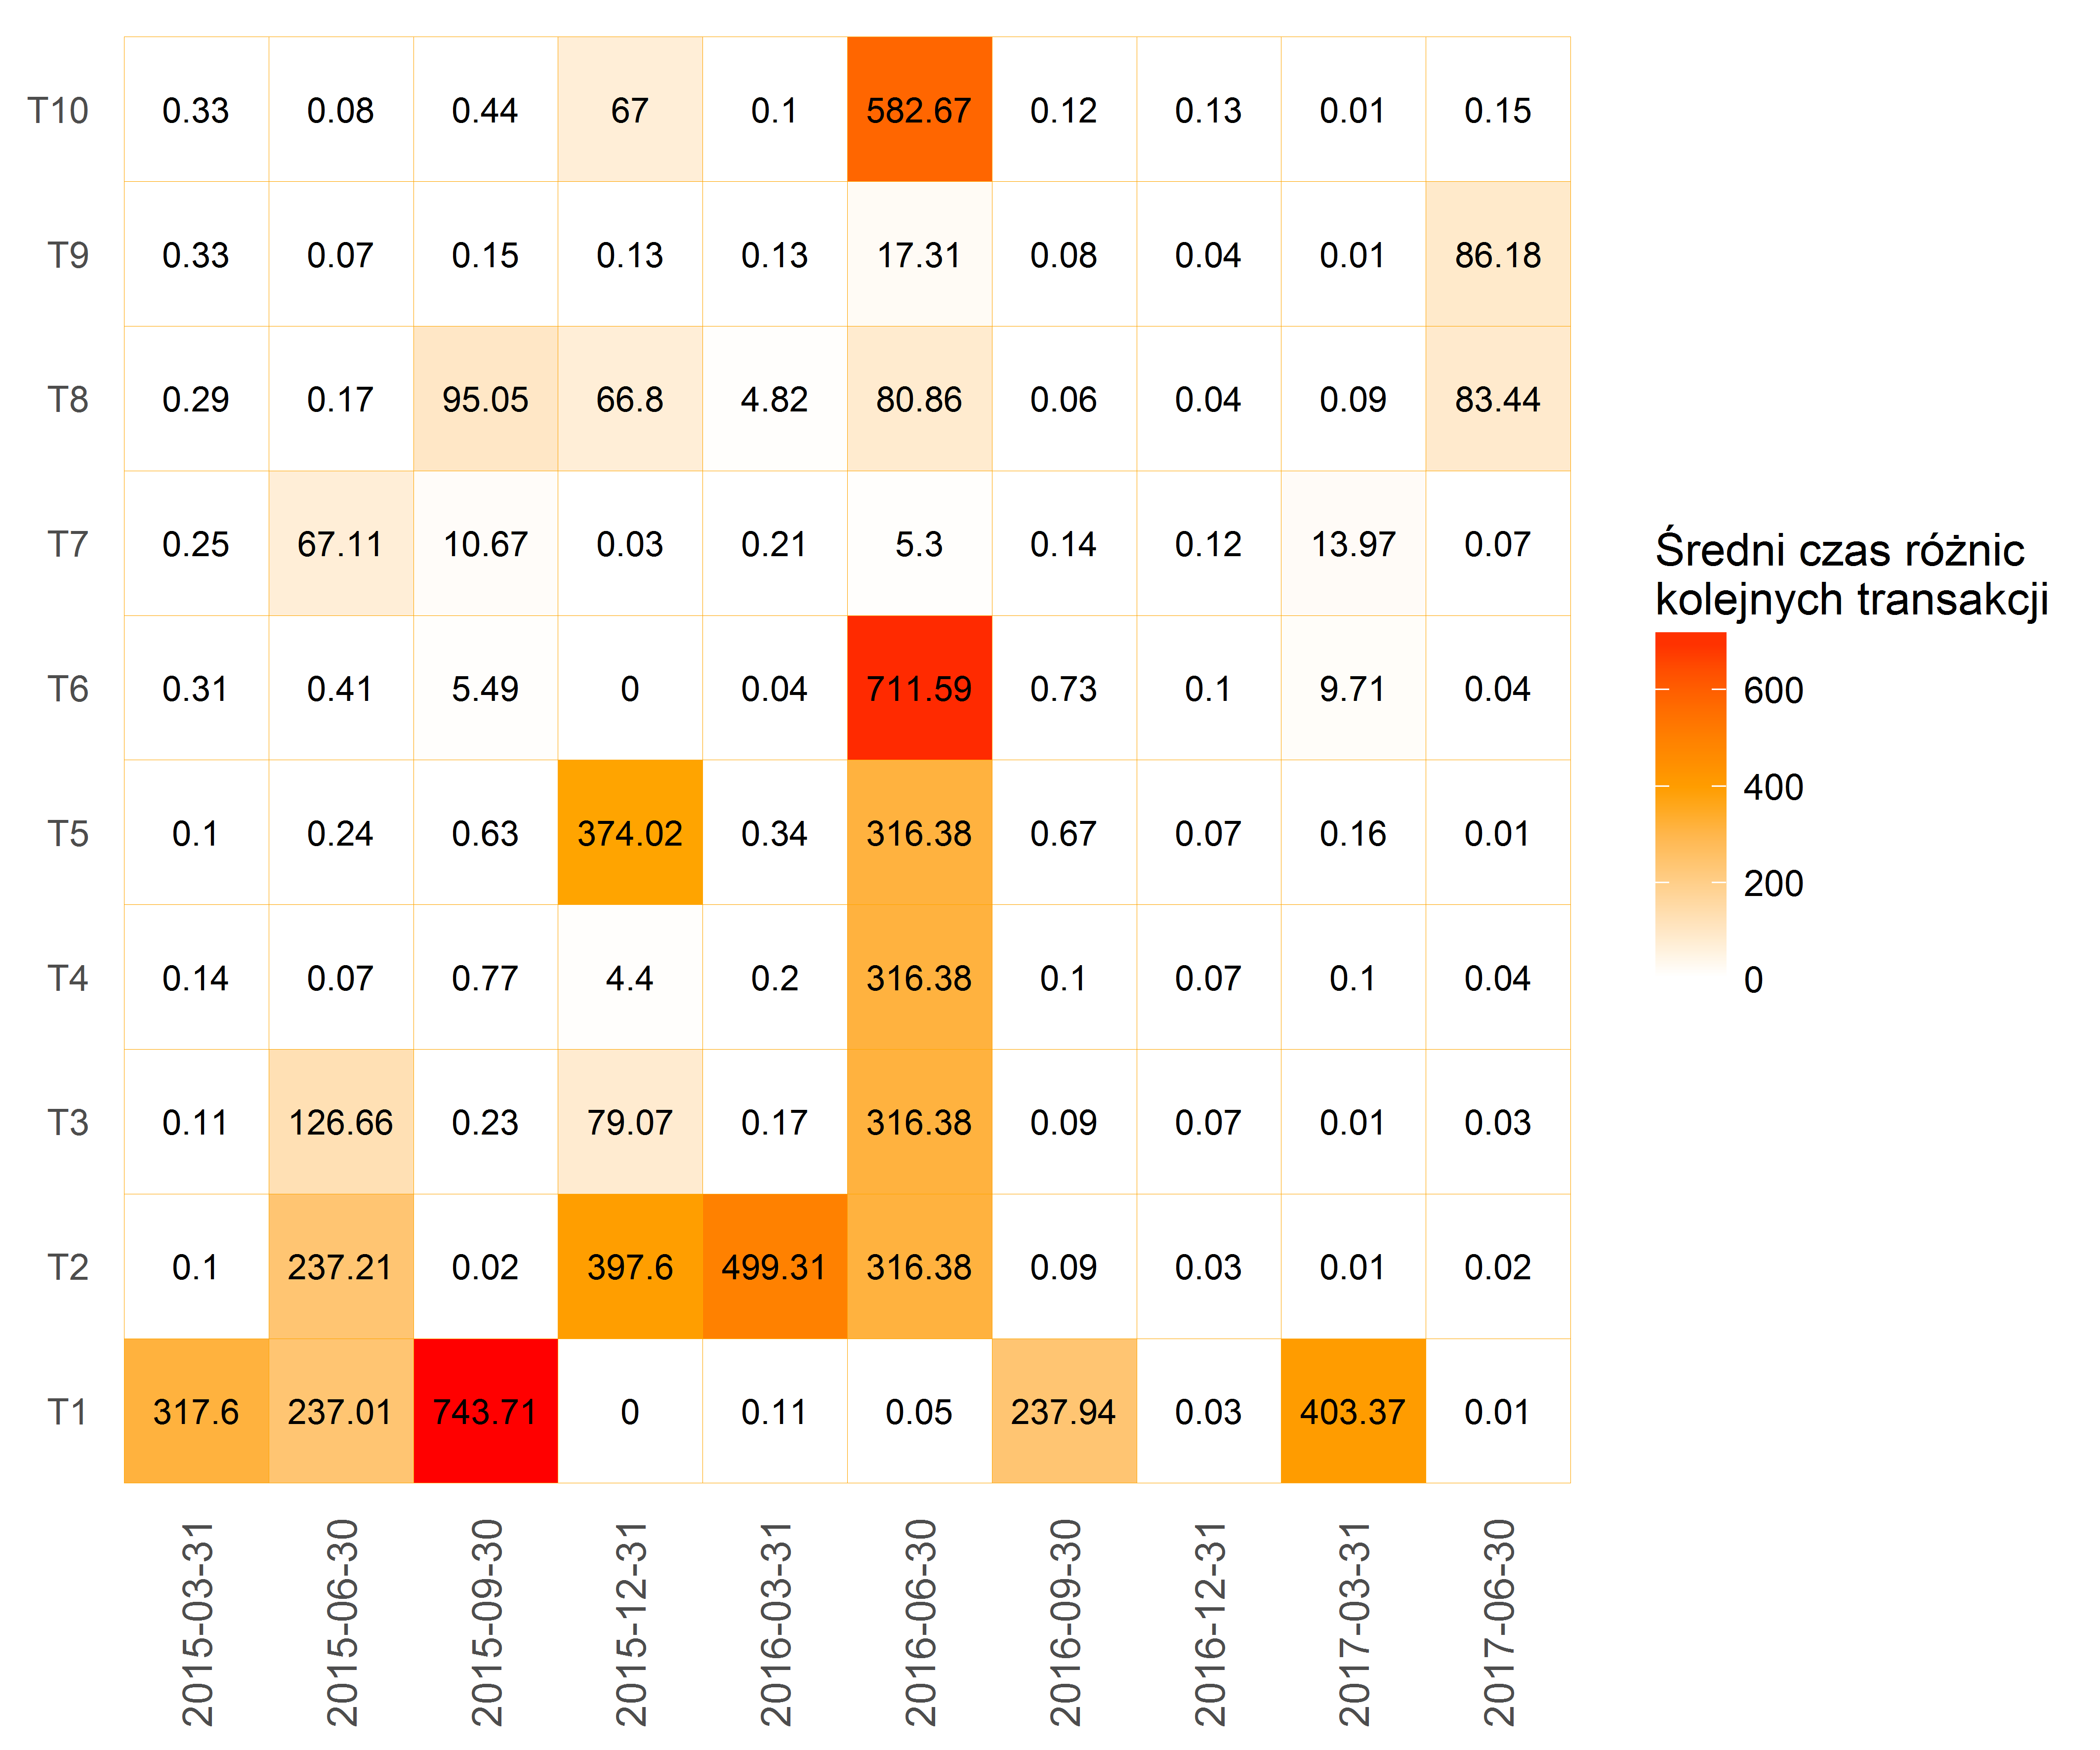
\includegraphics[width=\chartsWidth\linewidth]{pictures/roznica_czasow/roznica_czasow_hm.png}
   \caption{Mapa cieplna średniej różnicy czasu kolejnych transakcji sieci dla 10 prób w 10 okresach.}
   \label{fig:rc1} 
\end{figure}
\begin{figure}[H]
\centering
   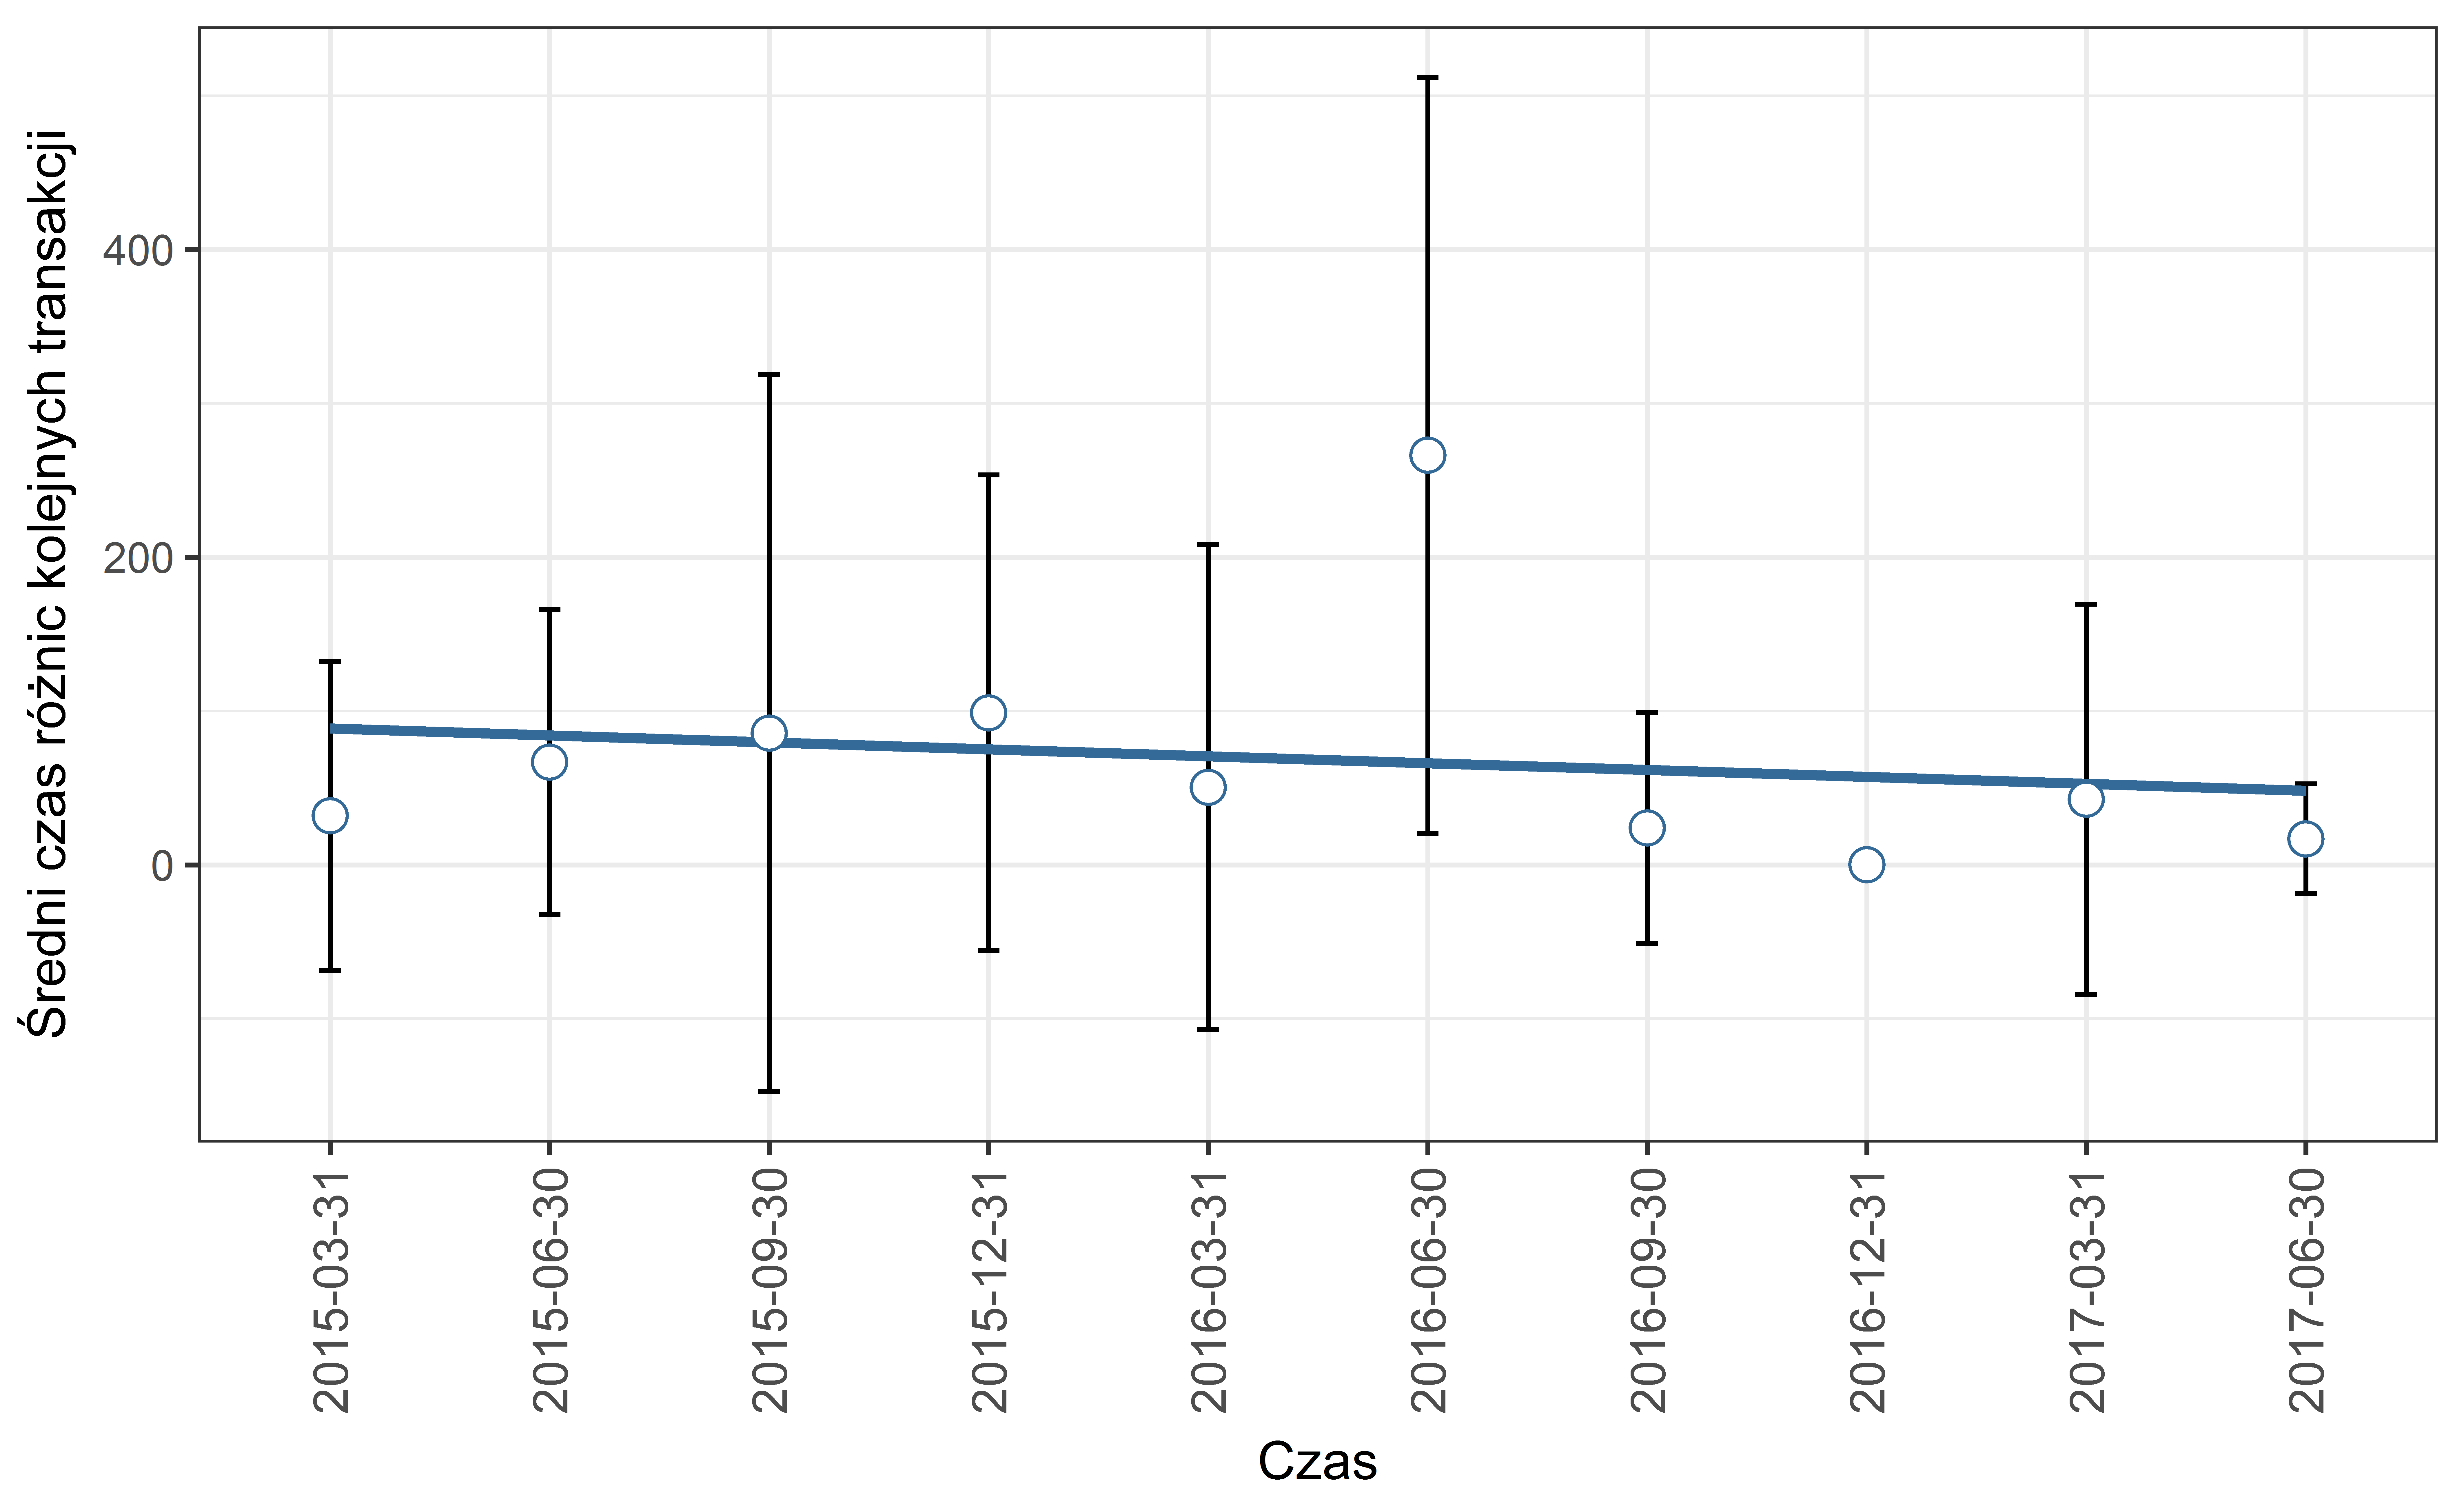
\includegraphics[width=\chartsWidth\linewidth]{pictures/roznica_czasow/roznica_czasow_sda.png}
   \caption{Regresja liniowa średniej różnicy czasu kolejnych transakcji sieci dla 10 okresów z odchyleniem standardowym.}
   \label{fig:rc2}
\end{figure}

\newpage
\subsection{Badanie różnicy czasów granicznych transakcji}
\label{graniczne_transakcje}
\indent Badanie różnicy czasów granicznych transakcji jest właściwością sieci bezpośrednio związaną z jej specyfiką. Polega na odnalezieniu wśród wszystkich możliwych ścieżek takiej ścieżki, której różnica czasów pierwszej oraz ostatniej transakcji jest największa. Jako że próby przygotowane w celu przeprowadzenia serii badań powstały od określonych transakcji $t$, czasem wykonania pierwszej transakcji będzie zawsze czas wykonania transakcji początkowej $t$. Różnica czasu wykonania transakcji początkowej $t$ oraz ostatniej transakcji dołączonej do danej ścieżki stanowi podstawę omawianego badania i może zostać przedstawiona jako
\begin{equation}
D(\sigma) = t(\sigma(v_1)) - t(\sigma(v_l))
\end{equation}
gdzie $D(\sigma)$ to różnica czasów wykonania transakcji, $t(\sigma(v_1))$ to czas wykonania pierwszej transakcji ścieżki, a $t(\sigma(v_l))$ to czas wykonania ostatniej transakcji ścieżki.
\\ Różnicę czasów granicznych transakcji można zatem zapisać jako
\begin{equation}
 \max_{\sigma_{st},s \ne t} D(\sigma_{st})
\end{equation}
gdzie $\sigma_{st}$ to ścieżka prowadząca od węzła $s$ do węzła $t$.

\indent Wyniki przeprowadzonego badania zaprezentowano na mapie cieplnej~\ref{fig:cg1}. Potwierdza ona wnioski opisane w~podrozdziale \ref{roznice_czasow} opisującym badanie różnic czasów kolejnych transakcji. Dla większości prób we wszystkich okresach zaobserwowano wykrycie wszystkich stu tysięcy połączeń pomiędzy transakcjami w bardzo krótkim czasie, determinując przegląd tylko kilku poprzedzających bloków. Różnica czasów granicznych transakcji dla próbek w okresach, których średni czas kolejnych transakcji znacząco odbiegał od średniej, jest największa. Potwierdza to sporadyczne realizowanie transakcji właścicieli adresów w~danych próbkach w okresie \textit{2016-06-30}. Na podstawie ostatnich czterech okresów wnioskować można, że aktualnie podobne sytuacje są rzadkością i~większość uczestników sieci realizuje znacząco więcej transakcji niż wcześniej, co potwierdza również wykres~\ref{fig:cg2}. Pozwala to na stwierdzenie, że sieć Bitcoin w przeciągu ostatnich czterech badanych okresów bardzo urosła i zyskała zaufanie większej liczby użytkowników.

\newpage
\begin{figure}[H]
\centering
   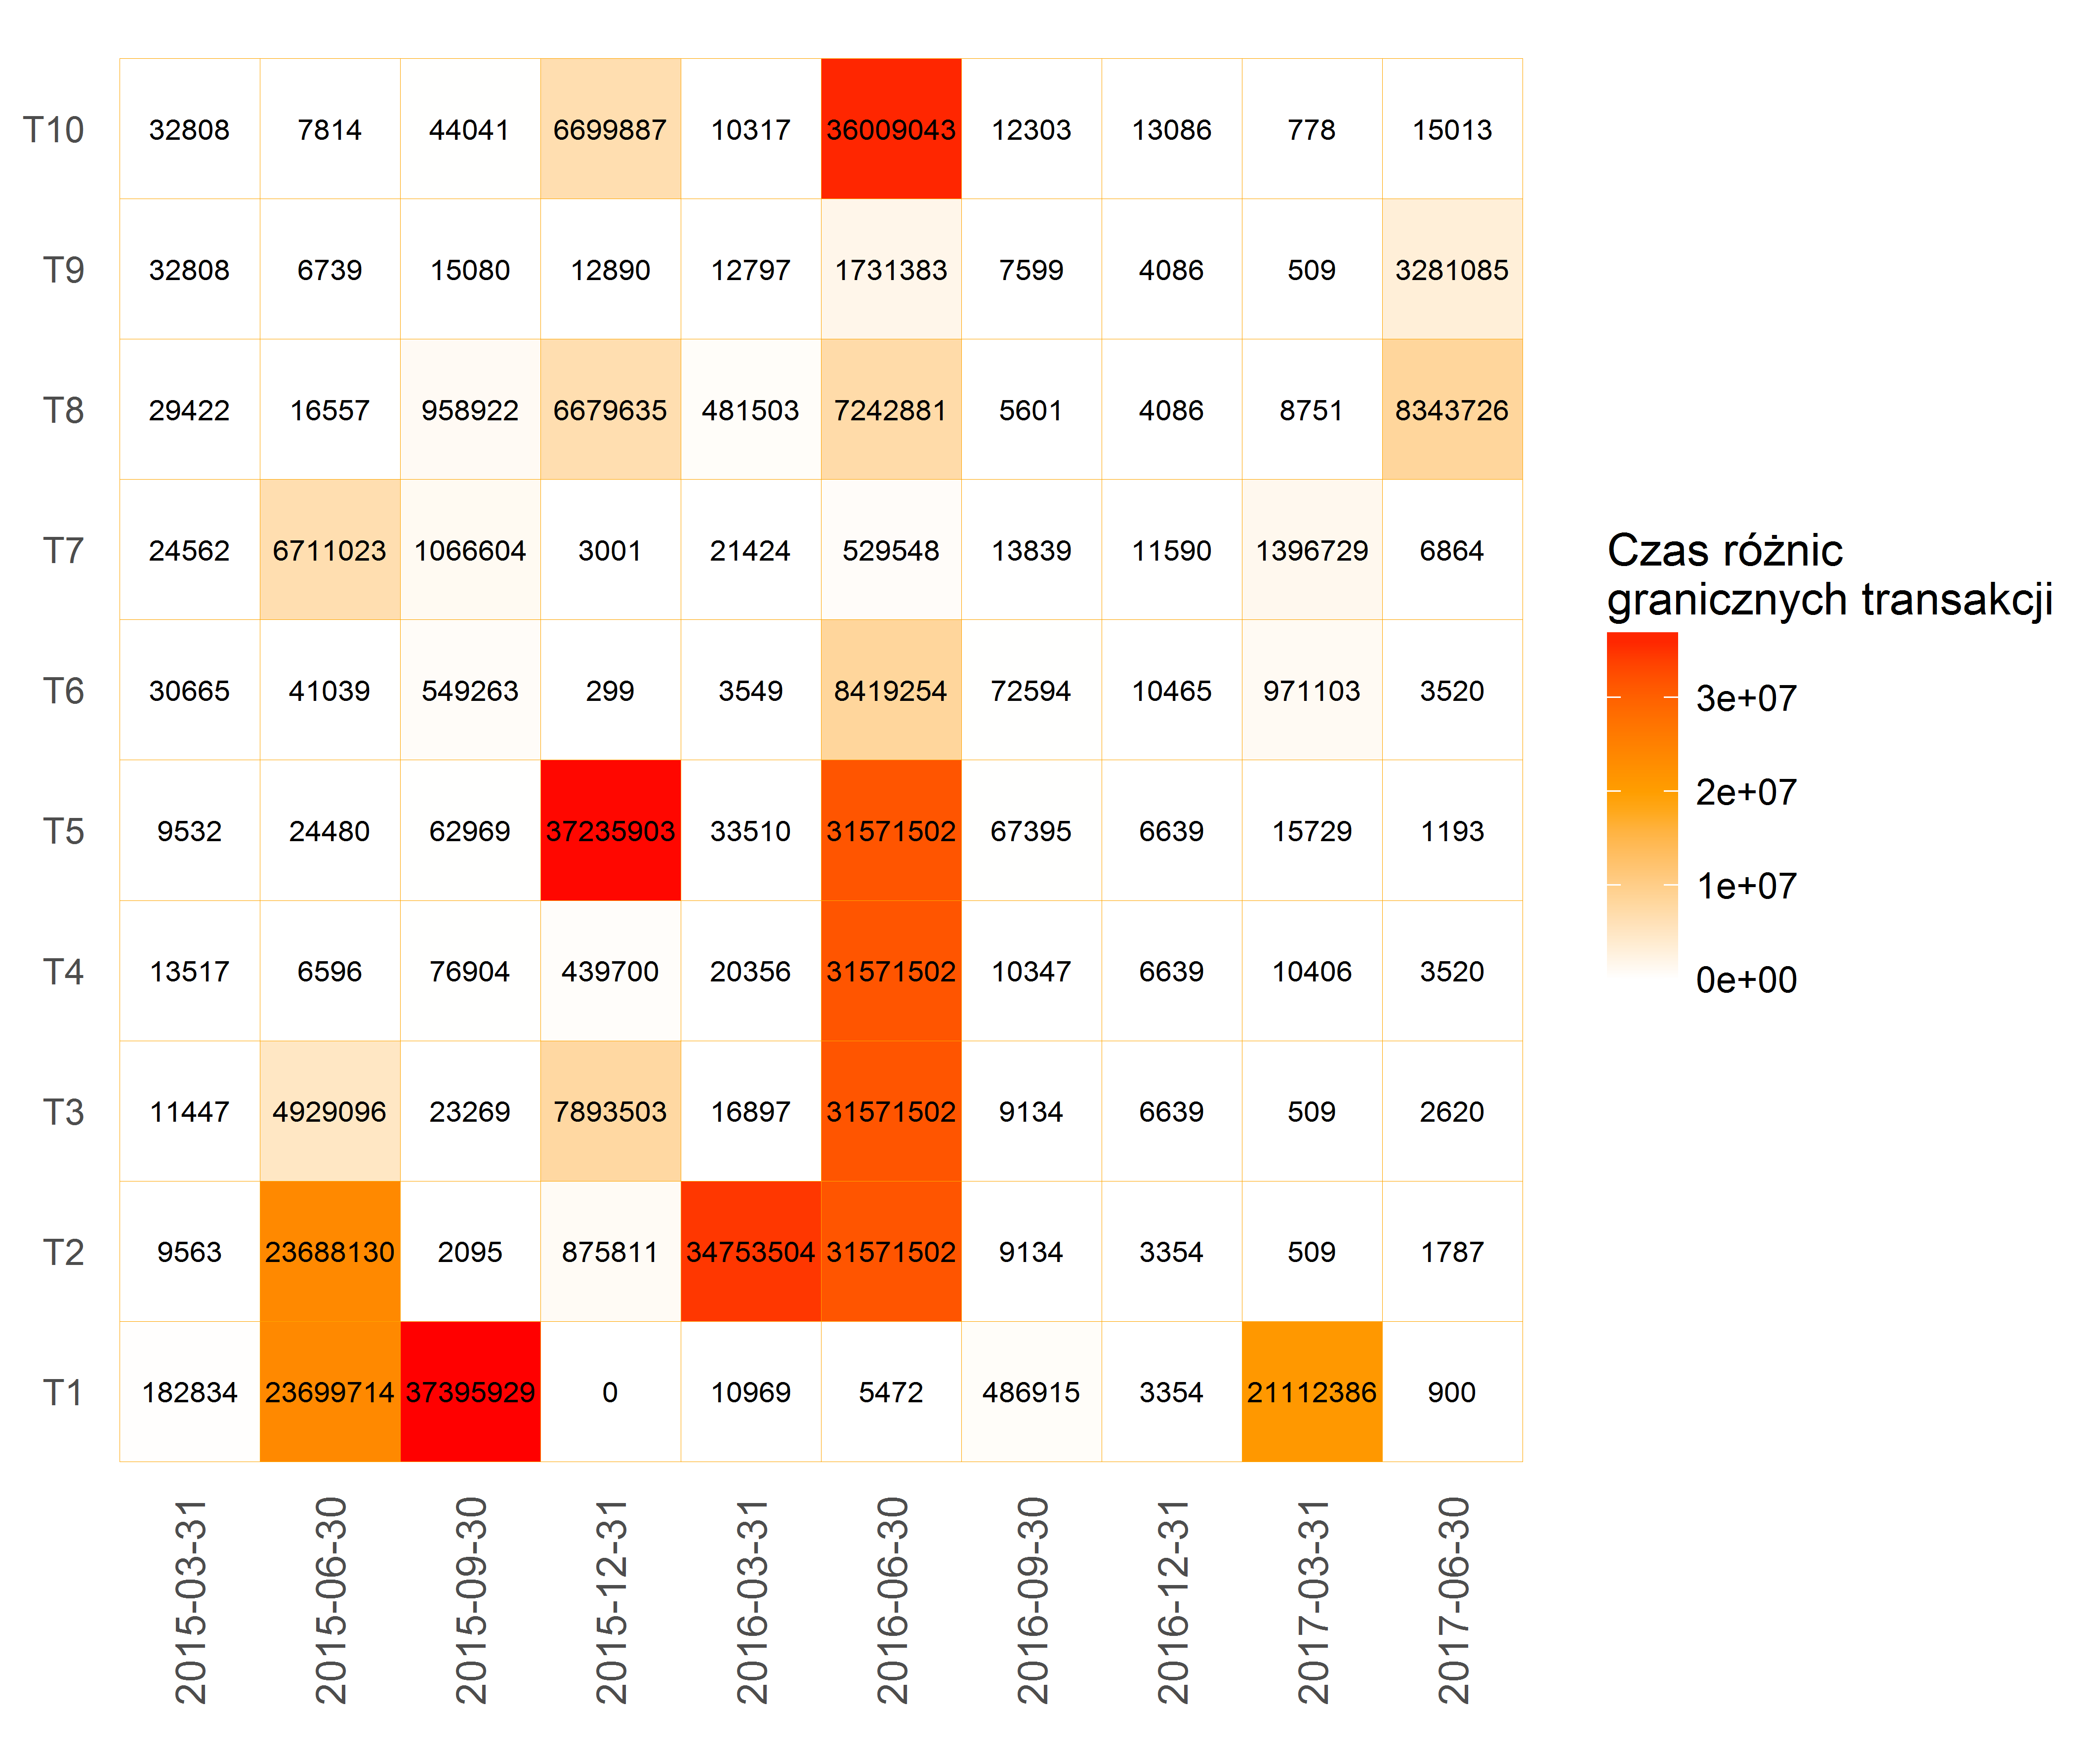
\includegraphics[width=\chartsWidth\linewidth]{pictures/czas_graniczny/czas_graniczny_hm.png}
   \caption{Mapa cieplna różnic czasu granicznych transakcji dla 10 prób w 10 okresach.}
   \label{fig:cg1} 
\end{figure}

\begin{figure}[H]
\centering
   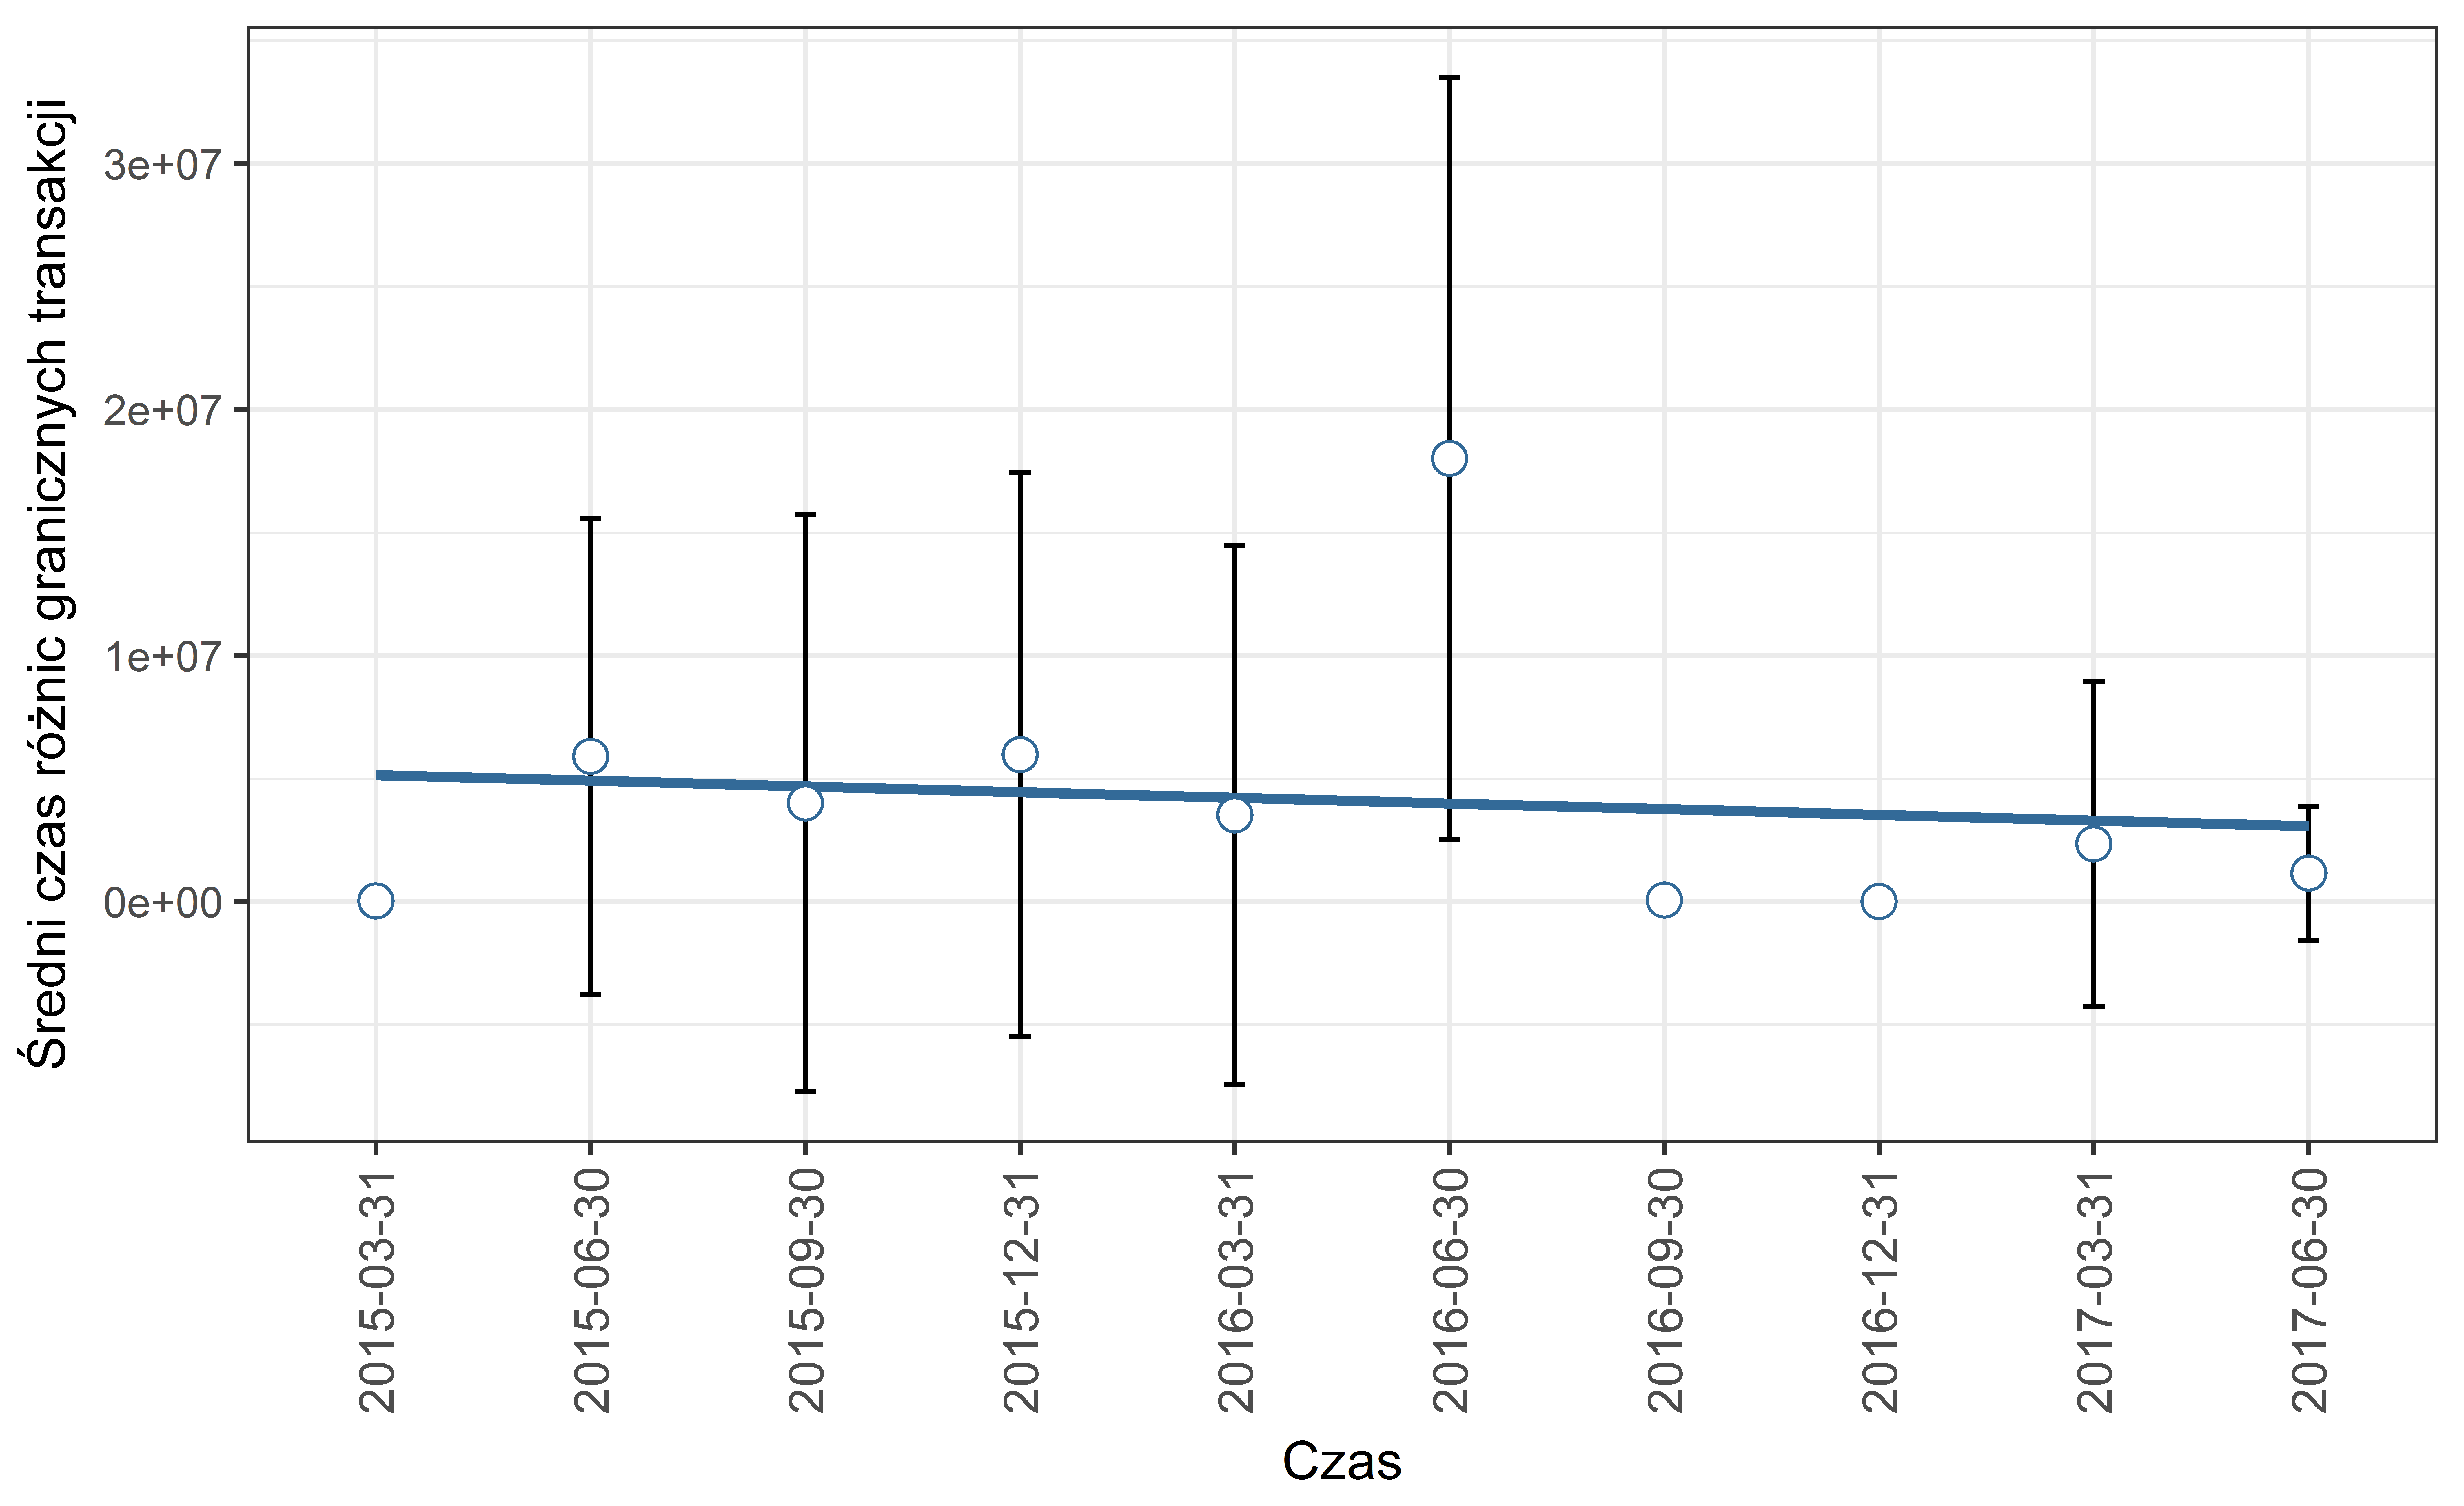
\includegraphics[width=\chartsWidth\linewidth]{pictures/czas_graniczny/czas_graniczny_sda.png}
   \caption{Regresja liniowa średniego różnic czasu granicznych transakcji dla 10 okresów z odchyleniem standardowym.}
   \label{fig:cg2}
\end{figure}

\newpage

\section{Wnioski}

Sieć Bitcoin jest bardzo złożoną, dynamiczną i szybko rozwijającą się siecią. Na podstawie przeprowadzonych badań wywnioskowano ciągle rosnącą gęstość sieci, co w odniesieniu do jej specyfiki oznacza coraz większą ilość zlecanych transakcji, powstawanie dużej ilości nowych adresów oraz wzrost realizowanych transakcji pomiędzy różnymi uczestnikami sieci. W podrozdziale~\ref{srednica_sieci} zjawisko to zostało przedstawione bardziej szczegółowo. Badanie centralności węzłów opisane w~podrozdziale~\ref{srednia_centralnosc} pozwoliło na zarejestrowanie znaczącego spadku istotności pojedynczej transakcji w całej sieci, co ponownie potwierdza fakt rosnącej ilości zlecanych transakcji. Zaobserwowano również, że właściwości sieci nie są stałe w~jednym okresie, a zależeć mogą od aktywności poszczególnych uczestników, dlatego też ilość połączeń pomiędzy transakcjami może być bardzo zróżnicowana, co zaprezentowano w podrozdziałach~\ref{dlugosc_sciezki}~i~\ref{stopien_wezla}. 

\indent W~trakcie badania poszczególnych próbek zauważono wzmożoną działalność pojedynczych właścicieli adresów, którzy zlecali lub odbierali znaczne sumy bitcoinów. Z~powodu dużej anonimowości w~sieci nie da się wprost określić właścicieli użytych adresów w tych transakcjach, chyba że są to adresy publiczne, których właściciele przyznają się do ich posiadania. Przypuszczać można jednak, że mogą to być adresy należące do dużych instytucji lub giełd, co potwierdzono w ~\ref{wartosc_transakcji}. Dodatkowo na podstawie analizy średniej wartości transakcji zauważono, że wartość większości transakcji nie przekracza 100 bitcoinów, a zazwyczaj są to małe przekazy środków pomiędzy klientami sieci. Porównanie wyników średnich wartości transakcji dla okresów w podrozdziale~\ref{wartosc_transakcji} pozwala stwierdzić, że ilość przekazywanych bitcoinów w transakcjach cały czas rośnie. Badanie ilości bloków potrzebnych do odnalezienia 100 tysięcy połączeń, w~powiązaniu z~analizą średniej różnicy czasów kolejnych transakcji oraz różnicy czasów transakcji granicznych (opisane kolejno w podrozdziałach~\ref{ilosc_blokow},~\ref{roznice_czasow},~\ref{graniczne_transakcje}), ilustruje wielkość oraz tempo rozwoju badanej sieci. W~ostatnich okresach transakcje do prób zostały odnalezione w~kilku blokach, a~różnice czasów granicznych transakcji zawartych w~próbach nie przekraczają kilkudziesięciu minut. W~rezultacie pozwala to na wywnioskowanie o~kolejności występowania po sobie bloków, w~których odnaleziono połączenia pomiędzy transakcjami. Odnalezienie tak olbrzymiej ilości powiązanych transakcji w~paru kolejnych blokach potwierdza rosnącą ilość realizowanych transakcji pomiędzy różnymi uczestnikami sieci w bardzo ograniczonym czasie.

\indent Reasumując, sieć Bitcoin jest siecią bardzo dynamicznie się rozwijającą. Można przypuszczać, że coraz więcej użytkowników używa jej jako codziennego medium transmisyjnego środków, a rosnącą gęstość sieci świadczy o rosnącej ilości samych użytkowników. 


\chapter*{Podsumowanie}
\addcontentsline{toc}{chapter}{Podsumowanie}  

\indent Prezentowana praca magisterska obejmuje wprowadzenie do kryptowalut na podstawie sieci Bitcoin, opis sposobu działania Blockchain'a oraz analizę sieci transakcji - główny cel pracy. Dzięki wykorzystaniu opisanego w pracy sposobu próbkowania sieci udało się zbudować sto prób sieci po sto tysięcy węzłów każda. Zastosowanie narzędzi badania opartych na metodach badania temporalnych sieci złożonych pozwoliło na pozyskanie informacji na temat różnych właściwości sieci. W przeprowadzonym eksperymencie pozyskano dane opisujące sieć pod względem ośmiu rożnych cech. Metody badania podzielono na dwie grupy, to znaczy na właściwości wynikające z struktury oraz tematyki badanego obiektu. W ramach metod badania struktury sieci przeanalizowano średnicę sieci, średnią długość ścieżki, średni stopień węzła oraz średnią centralność węzła każdej próby. Pozwoliło to na określenie między innymi gęstości sieci i znaczenia pojedynczego węzła na istnienie całej sieci. W zakresie badań wynikających z tematyki zbadano średnią wartość transakcji, liczbę bloków potrzebną do stworzenia próby, średnią różnicę czasu kolejnych transakcji oraz różnice czasu granicznych transakcji. Podzielenie prób na okresy umożliwiło określenie trendów zmian w całej sieci. Poprzez dodatkową analizę anomalii występujących w określonych próbach udowodniono możliwość odnalezienia adresów Bitcoin należących do giełd.

\indent Zaznaczyć należy, że przedstawiona w niniejszej pracy problematyka nie wyczerpuje w~całości zagadnienia dotyczącego ekstrakcji cech sieci transakcji w kryptowalucie Bitcoin oraz analizy Blockchain'a. Sieć Bitcoin cały czas ewoluuje i rośnie, co oznacza możliwość pozyskiwania coraz to innych właściwości. W pracy nie przeanalizowano wszystkich możliwych cech, jednakże pokazano, że istnieje taka możliwość przy zastosowaniu opisywanych technik badawczych. Coraz to nowe zastosowania Blockchain'a aktywizują do przeprowadzania kolejnych badań.

\indent Jedną z prac, która mogłaby być kontynuacją niniejszej jest stworzenie klasyfikatora dla adresów Bitcoin pozwalającego na identyfikację adresów należących na przykład do giełd. Większość giełd chcąc być wiarygodnym publikuje posiadane adresy Bitcoin. Dzięki temu przy pomocy technik budowania sieci zastosowanych w tej pracy możliwe jest stworzenie prób rozpoczynających się od transakcji wykonanych z adresów giełd. Analiza tych prób za pomocą metod użytych w niniejszej pracy pozwoliłaby na określenie zakresów wartości danych właściwości, a to w konsekwencji pozwoliłoby na budowę klasyfikatora.

\bibliographystyle{unsrt}
\addcontentsline{toc}{chapter}{Bibliografia}
\bibliography{bibliografia}

\listoffigures
\listoftables
\end{document}

% kropka za numeracja
% 
